\documentclass{article}
\IfFileExists{microtype.sty}{\usepackage[final]{microtype}}{}
\IfFileExists{xurl.sty}{\usepackage{xurl}}{}
\usepackage[margin=1in]{geometry}
\usepackage{booktabs}
\usepackage{graphicx}
\usepackage{url}
\usepackage{hyperref}
\usepackage{amsmath}
\usepackage{enumitem}
\IfFileExists{xr-hyper.sty}{%
  \usepackage{xr-hyper}%
  \IfFileExists{main.aux}{\externaldocument[][nocite]{main}}{}%
}{%
  \IfFileExists{xr.sty}{%
    \usepackage{xr}%
    \IfFileExists{main.aux}{\externaldocument{main}}{}%
  }{}%
}
\setlength{\emergencystretch}{5em}
\hbadness=10000
\hypersetup{
  pdftitle={Supplementary material to SPOT-OD: Adaptive-Filter and Observability Mechanism Findings from a Simulator-Bound Orbit-Determination Audit},
  pdfauthor={Authors omitted for review},
  pdfsubject={Supplementary material for the SPOT-OD orbit determination audit manuscript},
  pdfkeywords={orbit determination, satellite state estimation, sparse visibility, graph neural networks, learned filtering, supplementary material, reproducibility}
}

\title{Supplementary material to ``SPOT-OD: Adaptive-Filter and Observability Mechanism Findings from a Simulator-Bound Orbit-Determination Audit''}
\author{Authors omitted for review}
\date{June 2026}

\begin{document}
\maketitle
\renewcommand{\tablename}{S-Table}
\renewcommand{\figurename}{S-Figure}

\noindent This supplementary document accompanies the main manuscript. The printable supplement provides the complete learned-estimator architecture/training specification, full table bodies for core and boundary-audit material, and concise indexed summaries for selected lower-priority archival records; full numeric tables for those selected lower-priority records are supplied in the confidential journal-review evidence package. Cross-references to main-text sections, tables, and figures are given by label; numeric values are preserved verbatim from the reported result records.

\paragraph{Cross-document numbering convention.}
Before any numeric citation is used below, note that the supplement is a standalone document and maintains its own reference list. The supplement's reference numbering is independent of the main manuscript's numbering: a citation such as [6] in the supplement and [33] in the main manuscript can refer to the same source entry, and a reader should not rely on numeric cross-document correspondence. Supplement table entries may be printed table bodies or indexed evidence-package records, labelled S-Table~$N$; figures are labelled S-Figure~$N$; main-manuscript objects keep their unprefixed names. References from this supplement to a main-manuscript section, table, or figure are given by descriptive name and symbolic label rather than as a bare number. Where the identity of a cited source matters for disambiguation, we name the source explicitly alongside the citation. For the CRLB floor derivation, the Tapley--Schutz--Born statistical-OD source uses the shared key \texttt{tapley2004statistical}; only the printed reference number may differ between the standalone supplement and main paper. The canonical identifiers of each source are the unchanging citation keys shared between the two documents.

\paragraph{Reader route.}
Readers checking the headline claims should start with the main manuscript's claim--evidence--limit hierarchy (main Table~\ref{tab:main_claim_evidence_limit}). Section~\ref{app:predeclaration-excerpts} gives non-confidential excerpts from the primary decision records and separates the load-bearing and non-evidentiary tiers. In this supplement, Sections~\ref{app:floor-sensitivity-and-stability}--\ref{app:structural-channel-recoverability} support the structural-channel decision floors and sanity diagnostics; Section~\ref{app:kalmannet-spot-od-feasibility} records the KalmanNet transposition route and its bounded outcome; Section~\ref{app:novelty-audit-systematic} supports the scoped positioning audit; and Section~\ref{app:supplementary} houses the demoted, diagnostic, public measurement-pipeline/provenance, and reproducibility-support tables. The supplementary evidence materials link headline statements to descriptive claim records and inspection checks. Public ILRS/SP3 probes are measurement-pipeline/provenance checks only; they are not operational POD validation or external confirmation of the simulator conclusion.

\paragraph{Supplement table guide.}
Readers checking the headline claims need only the \textbf{core} tiers (items 1--3 below); items 4--7 are archival/diagnostic records that bound interpretation and are not required to evaluate the primary conclusions.
Readers whose primary interest is novelty or boundary adjudication should proceed directly to \textbf{Archival~7} (item 7 below), which consolidates the systematic novelty audit, subset-sufficiency map, claim hierarchy, and nearest-literature checks; Core~1--3 carry the empirical headline but do not repeat that boundary evidence.
The 68+ S-tables are grouped by evidentiary role:
\begin{description}[nosep, itemsep=2pt, leftmargin=0pt, labelindent=0pt]
  \item[\textbf{Core 1---Load-bearing hierarchy.}]
    Endpoint checks, powered stress check, and primary bounded negatives.
    Sec.~\ref{app:predeclaration-excerpts}; S-Tables~\ref{tab:protocol_subset_ablation}--\ref{tab:long_arc_hifi_force_mismatch}.
  \item[\textbf{Core 2---Decision-floor support.}]
    Floor sensitivity, stability, and favorable-geometry sanity checks.
    Secs.~\ref{app:floor-sensitivity-and-stability}--\ref{app:structural-channel-recoverability}; S-Tables~\ref{tab:crlb_floor_sensitivity}--\ref{tab:structural_channel_recoverability}.
  \item[\textbf{Core 3---Mechanism diagnostics.}]
    AUKF force-mismatch mechanism and drag-scale observability cascade.
    Secs.~\ref{app:constructive-positive-control}--\ref{app:observability-positive-control-ukf}; S-Tables~\ref{tab:force_mismatch_mechanism}, \ref{tab:hifi_force_mismatch}, \ref{tab:drag_scale_constructive_positive_control}--\ref{tab:drag_scale_ukf_observability_positive_control}.
  \item[Archival 4---Learned-comparator bounds.]
    KalmanNet-lineage, residual-bound, selection-pathway, ablation, and seed-cohort checks.
    Sec.~\ref{app:kalmannet-spot-od-feasibility}; S-Tables~\ref{tab:measurement_informed_results}, \ref{tab:kalmannet_official_reproduction}, \ref{tab:seed_aware_significance}--\ref{tab:residual_scale_sweep}, \ref{tab:ablation}--\ref{tab:satnogs_selection_sensitivity}.
  \item[Archival 5---Public and classical probes.]
    Public-catalog replay, ILRS/SP3 state scoring, dense tracking, offline OD, and smoothing references.
    Sec.~\ref{app:supplementary}; S-Tables~\ref{tab:credible_dense_od_probe}--\ref{tab:dense_tracking_tail_audit}, \ref{tab:public_data_summary}--\ref{tab:correction_component_audit}, \ref{tab:propagation_baseline}--\ref{tab:pure_gnn_training_sanity}.
  \item[Archival 6---Diagnostic robustness.]
    Coverage, calibration, multiplicity, practical-floor, observability, engineering-failure, and robustness summaries.
    Sec.~\ref{app:supplementary}; S-Tables~\ref{tab:multiplicity_adjusted}, \ref{tab:floor_sensitivity_sweep}, \ref{tab:coverage_runtime}--\ref{tab:significance}, \ref{tab:engineering_failure}--\ref{tab:robustness}.
  \item[Archival 7---Boundary audit.]
    Novelty, subset sufficiency, claim hierarchy, and nearest-literature checks.
    Sec.~\ref{app:novelty-audit-systematic}; S-Tables~\ref{tab:novelty_audit_systematic}--\ref{tab:near_miss_audit}.
\end{description}

\paragraph{Abbreviation glossary.}
\begin{center}
\scriptsize
\begin{tabular}{p{0.20\linewidth}p{0.72\linewidth}}
\toprule
Abbreviation & Meaning in this manuscript \\
\midrule
AUKF & Adaptive unscented Kalman filter with innovation-based measurement-noise scaling. \\
CRLB & Cram\'er--Rao lower bound used as an approximate practical decision floor. \\
DBAR & Diagnostic bounded adaptive-filter risk heuristic; characterized and withdrawn. \\
DMC-EKF & Dynamic-model-compensation EKF with empirical-acceleration state augmentation. \\
DSA-EKF / DSA-UKF & Drag-scale augmented EKF / UKF structural-channel diagnostic. \\
EKF / UKF & Extended Kalman filter / unscented Kalman filter. \\
ILRS / SLR / SP3 & International Laser Ranging Service / satellite laser ranging / precise-orbit state product format. \\
NIS & Normalized innovation squared. \\
OD / POD & Orbit determination / precise orbit determination. \\
PUKF & Process-noise adaptive UKF. \\
RFIS / VG-RFIS & Robust fixed-interval smoother / visibility-gated RFIS composite. \\
RGR-GF & Residual graph recurrent estimator with graph filtering priors. \\
RGR-local / RGR-noMP / RGR-U & Capacity-matched local control / no-message-passing control / unconstrained residual comparator. \\
SGP4 & Simplified General Perturbations 4 public-catalog propagation model. \\
SPOT-OD & Sparse-visibility Protocol for Orbit-determination Testing. \\
WLS & Robust batch weighted least-squares orbit-determination reference. \\
\bottomrule
\end{tabular}
\end{center}

\section{Primary decision-record excerpts and evidence hierarchy}
\label{app:predeclaration-excerpts}

This section makes the key decision-record language visible in the manuscript package. The records are internal records rather than external public preregistration, so they provide inspectability and digest consistency, not the same assurance as an external registry; the central $K=32$ record is timestamped, while the earlier $K=8$ endpoint-fixation support record lacks a created/finalized timestamp field. Observed-step RMSE first surfaced in a training-cohort post-hoc recomputation; the $K=8$ record then checked that selected endpoint, a later strict-prefix extension was a non-evidentiary response to borderline $K=8$ intervals, and the $K=32$ rule was fixed only after those records but before any $K=32$ draw. A later stress-only $K=96$ record was fixed before its own draw to test the stress row at the floor-power scale. The current claim hierarchy is:
\begin{enumerate}[leftmargin=*]
  \item \textbf{Central anchor:} the $K=32$ frozen-rule observed-step replication under the $K=8$-established endpoint hierarchy, fixed before the new $K=32$ draw and reported in the main text.
  \item \textbf{Powered stress-row check:} the stress-only $K=96$ frozen-rule replication, fixed before the K=96 stress draw and reported as a supplementary floor-power-scale check.
  \item \textbf{Endpoint-fixation support:} the $K=8$ strict-prefix endpoint-fixation result, reported as a supporting rule check with no created/finalized timestamp asserted.
  \item \textbf{Non-evidentiary audit trail:} the later strict-prefix extension. Because it was triggered after seeing borderline $K=8$ intervals, it has no predeclared or confirmatory status and is excluded from the evidence hierarchy.
\end{enumerate}

\paragraph{Central $K=32$ frozen-rule record.}
The retained decision record for the larger independent endpoint replication states that the rule was fixed at 2026-05-21T19:26:19.5401506+02:00 before evaluation, uses base seed 880000, evaluates $32$ independent realizations per scenario and $24$ trajectories per realization, and uses $5000$ bootstrap samples. Its primary metric is ``observed-step position RMSE''; its reference metric is ``all-step position RMSE''. The statistical unit is an independent realization with an independently seeded trajectory population and measurement-noise draw. The decision predicate is:
\begin{quote}\small
For each scenario, estimate the mean observed-step position RMSE over independent realizations. Compute the paired gap as RGR-GF observed-step position RMSE minus the best classical observed-step position RMSE in the same realization. A learned positive requires RGR-GF to be the lowest-mean method for the scenario and the upper endpoint of the paired-gap confidence interval to be strictly below zero. The all-step metric is reported only as a propagation-dominated reference and is not part of the decision predicate.
\end{quote}
The same record also states that the fixed, previously trained learned estimator is used in inference only, with no model selection, tuning, or retraining, and that the base seed is disjoint from the training/validation cohort, model-selection validation splits, the earlier endpoint-fixation seed, and the scenario-resampling seed. Its interpretation boundary states that this is a larger independent endpoint replication, not an external preregistration record.

\paragraph{Timeline relative to endpoint fixation.}
The $K=32$ record was fixed after the study had already adopted observed-step RMSE from the endpoint-fixation pathway, after the $K=8$ endpoint-fixation record existed, and after the non-evidentiary strict-prefix extension had been inspected; it is not an external preregistration and is not represented as earlier than the $K=8$ record. The $K=8$ endpoint-fixation record is the earlier submitted endpoint-fixation JSON record identified as the observed-step endpoint-fixation support record. The endpoint-fixation record predates the larger replication but was produced by an earlier record format that did not include a created/finalized timestamp field; consequently the manuscript cites the submitted record identity and does not assert a timestamp for it. That absent timestamp is an evidentiary limitation of the $K=8$ support record, while the timestamped central anchor is the later $K=32$ frozen-rule replication. The $K=32$ evidentiary role is narrower: it freezes a larger, seed-disjoint replication rule before any $K=32$ realization was generated or evaluated, and it excludes model selection, tuning, retraining, or metric substitution. The strict-prefix extension remains non-evidentiary because it was triggered by borderline $K=8$ intervals; the $K=32$ record is reported separately as a seed-disjoint frozen-rule replication under the established endpoint hierarchy rather than as a pre-$K=8$ preregistration.

Compact evidence-pipeline timeline:
\begin{enumerate}[leftmargin=*]
  \item Observed-step RMSE first surfaced in a training-cohort post-hoc recomputation.
  \item The observed-step endpoint-fixation record adopts observed-step RMSE as the primary endpoint and all-step RMSE as a propagation-dominated reference.
  \item The fixed $K=8$ endpoint-fixation draw supports the same no-learned-positive ordering under that endpoint hierarchy.
  \item The strict-prefix extension is triggered by borderline $K=8$ intervals and retained only as a non-evidentiary audit trail.
  \item The larger $K=32$ frozen-rule record is fixed at 2026-05-21T19:26:19.5401506+02:00, after the $K=8$ support record and the non-evidentiary extension and before any $K=32$ realization is generated or evaluated.
  \item The $K=32$ evaluation is then run as a seed-disjoint frozen-rule replication.
\end{enumerate}

\paragraph{$K=32$ power interpretation for the 3\% floor.}
The $K=32$ replication uses independent realization means as the statistical unit; independence refers to separately seeded trajectory populations and measurement-noise draws, not to trajectory steps within a pass. Using the realized paired-gap standard deviations as a descriptive design check, a one-sided $t$-approximation at $\alpha=0.05$ gives approximate power of $0.42$ for a stress-row effect exactly equal to the 3\% floor (27.5~m relative to AUKF); the realized stress gap of 48.8~m exceeds that floor. Power is reported at the predeclared floor effect rather than at the realized gap, since power computed at an observed effect is a deterministic function of the realized $p$-value. Because the decision predicate is the stricter two-sided 95\% CI upper-bound rule (effective one-sided $\alpha=0.025$), the realized floor power is somewhat below this figure and the required $K$ somewhat above the value below. With the realized stress-row paired-gap SD of 106.2~m, the same approximation reaches about 0.80 power for the 27.5~m stress-floor effect at $K\approx94$ independent realizations. The controlled-mismatch row gives approximate power of $0.79$ for its 3\% floor (14.2~m relative to EKF); its realized gap of 16.8~m also exceeds that floor. The nominal row remains underpowered for floor-scale interpretation. The 3\% floor is a mission-agnostic audit threshold for the compact simulator, not a universal mission requirement; a mission-specific OD campaign would replace it with its own acceptance threshold. This is why the manuscript treats the stress and controlled-mismatch rows as discriminative negatives for their observed degradations, while it does not claim that $K=32$ would reliably detect every just-at-floor effect.

\paragraph{$K=32$ within-unit correlation and recurrence boundary.}
Each $K=32$ realization contains 24 freshly simulated trajectories generated from that realization's seed, with its own measurement-noise and initial-state perturbation draws; the design does not intentionally resample a finite stored trajectory pool across realizations. Under the continuous initial-state and noise perturbation draws used here, exact trajectory collision across the $K=32$ realizations has probability zero almost surely. The retained record does not store cross-realization trajectory identifiers, so no empirical recurrence rate is claimed. The confidence intervals are therefore interpreted at the $K=32$ realization-mean level. They should not be read as if the 768 trajectories, or the time steps within those trajectories, were independent inferential units.

\paragraph{Stress-only $K=96$ powered-rule record.}
The retained stress-focused rule fixes base seed 991117, evaluates only the measurement-noise stress scenario, uses $96$ independent realizations with $24$ trajectories per realization, and uses the same observed-step position-RMSE endpoint and paired RGR-GF-minus-best-classical decision predicate as the larger endpoint replication. The design explicitly exceeds the $K\approx94$ realization count needed by the prior one-sided $t$ approximation for approximately 0.80 power at the 27.5~m stress-floor effect. Internal timestamp evidence records the rule fixed at 2026-05-25T13:06:32Z and the archived $K=96$ evaluation-start timestamp at 2026-05-25T13:12:43.6581323Z, about six minutes later. The completed draw preserves the bounded negative: AUKF is the best observed-step method (923.5~m), RGR-GF is 955.5~m, and the paired RGR-GF-minus-AUKF gap is \(+31.9\)~m with a 95\% bootstrap interval \([+12.4,+52.4]\)~m. This is still an internal frozen-rule replication under an already selected endpoint, not external preregistration, public-reference validation, or operational validation.

\paragraph{Additional internal prospective replication.}
The evidence package additionally includes a further independently seeded internal prospective replication (base seed 1160000, $K=32$ independent realizations per scenario, 24 trajectories per realization). The rule is written to an internal frozen-rule record before any additional replication realization is generated or evaluated, under the same frozen decision predicate as the central $K=32$ anchor. The base seed is disjoint from the 41--55 training/validation cohort, all model-selection validation splits, the endpoint-fixation seed 770000, the central $K=32$ seed 880000, the stress-only $K=96$ seed 991117, and the scenario-resampling seed 90000. The completed replication is reported in S-Table~\ref{tab:observed_step_internal_prospective_replication}. The bounded negative and no-learned-positive outcome is preserved in all three scenarios. On the nominal split, EKF is the best classical reference (388.46~m) and RGR-GF records 391.71~m; the paired RGR-GF-minus-EKF gap is \(+3.25\)~m with a 95\% bootstrap interval \([-7.64,+18.24]\)~m; the nominal split remains non-discriminative at the 3\% practical floor and is retained for traceability only. On the measurement-noise stress scenario, AUKF is the best classical reference (958.41~m) and RGR-GF records 999.61~m; the paired gap is \(+41.21\)~m with interval \([+10.04,+74.97]\)~m, a strictly positive interval and a mean degradation above the 3 percent floor. On the controlled force-model mismatch scenario, EKF is the best classical reference (465.12~m) and RGR-GF records 487.57~m; the paired gap is \(+22.45\)~m with interval \([+14.91,+29.51]\)~m, the tightest interval of the three scenarios. In all three scenarios the learned positive criterion (RGR-GF strictly best mean and paired interval strictly below zero) is not met; 0 of 3 scenarios return a learned positive, and the best classical filter wins in all 3 scenarios. This record is an additional internal evidence check, not external preregistration, public-reference validation, or operational validation.

\paragraph{Confidential hash-timestamped $K=16$ replication.}
The evidence package additionally includes a later all-scenario $K=16$ replication (base seed 1840000) under the same frozen decision predicate. Before generating or evaluating any realization, the frozen rule hash was submitted to an RFC3161 timestamp authority; the request disclosed only the SHA-256 hash, not the rule or manuscript content. The RFC3161 timestamp response Date is Sun, 31 May 2026 23:59:17 GMT. The base seed is disjoint from all earlier seed bases. The completed replication is reported in S-Table~\ref{tab:observed_step_confidential_timestamp_k16}. The 0 of 3 scenarios learned-positive outcome is preserved across all three scenarios. This confidential timestamp is stronger than an internal timestamp for this draw but is not public preregistration, not external endpoint-family validation, and not operational validation. The timestamp does not upgrade the observed-step endpoint itself from post-hoc to externally predeclared.

\paragraph{Endpoint-fixation record.}
The endpoint-fixation record records the adoption of observed-step position RMSE as the primary endpoint and all-step RMSE as the propagation-dominated reference after the training-cohort post-hoc recomputation had surfaced the metric. Its decision rule states that a learned positive requires the fixed RGR-GF to be the per-scenario best method with the paired RGR-GF-minus-best-classical bootstrap interval strictly below zero. The manuscript uses only the $K=8$ strict-prefix subset as the endpoint-fixation support. The later strict-prefix extension is retained in the evidence package only to document the adaptive extension and is not used as a confirmatory result.

\section{CRLB-floor sensitivity audit and decision-stability analysis}
\label{app:floor-sensitivity-and-stability}

The long-arc held-out-test predeclared positive-criterion threshold is the approximate astrodynamics-grounded $106.0$~m Cram\'er--Rao floor under stated assumptions on the arc-accumulated 3D position-RMSE (derivation in Section~\ref{app:crlb-derivation}). The derivation contains floor-raising simplifications (minimum-elevation slant range and no credit for simultaneous multi-station observations beyond the visible-step count) and one less-conservative approximation (treating consecutive visible steps within a pass as independent, which can tighten the floor when within-pass residuals are temporally correlated). A reader may compute a tighter or looser effective-count variant and ask whether the predeclared pass/fail decisions are stable.

S-Table~\ref{tab:crlb_floor_sensitivity} reports a closed-form sensitivity audit over six variants of the dominant floor levers: the predeclared baseline; a tighter slant range evaluated at the mean visible elevation rather than at the minimum-elevation cap; the range-rate noise added in quadrature to the per-update position variance (a marginal perturbation at worst-case slant range; row~C returns the same 106.0~m floor); a multi-visibility credit factor of $1.25$; all three relaxations applied simultaneously; and a conservative pass-correlated effective-count bound that divides the baseline visible-step count by a 10-step (200~s) within-pass correlation block. Across all six variants the predeclared positive-criterion decision on the long-arc held-out test is preserved because the structural channel is not strictly lowest in mean under any variant. The floor magnitude is therefore not decision-critical to the DSA-EKF negative; the audit is informational and does not load-bear the predeclared rule.

\begin{table}[t]
  \centering\small
  \caption{CRLB-floor sensitivity audit for the long-arc held-out test. Rows B, D, and E report tighter floors from relaxing the conservative slant-range and multi-visibility assumptions; row C adds the range-rate noise in quadrature (a marginal perturbation that returns the same floor at worst-case slant range); row F reports a looser pass-correlated effective-count bound for within-pass temporal correlation. Across all six variants the predeclared positive criterion remains unsatisfied because the structural-channel mean is not strictly lowest, so the predeclared decision is floor-robust; the audit is informational and does not load-bear the predeclared rule.}
  \label{tab:crlb_floor_sensitivity}
  \begin{tabular}{p{0.30\linewidth}cccc}
    \toprule
    Variant & Floor [m] & Slant range [km] & Independent obs. & Decision flips? \\
    \midrule
    A. Predeclared baseline (worst-case slant range, no range-rate term, no-overlap union bound) & 106.0 & 2,307 & 116 & No \\
    B. Tighter slant range at mean visible elevation & 41.2 & 895 & 116 & No \\
    C. Range-rate noise term in quadrature & 106.0 & 2,307 & 116 & No \\
    D. Multi-visibility credit factor 1.25 & 94.8 & 2,307 & 145 & No \\
    E. All three relaxations combined & 36.8 & 895 & 145 & No \\
    F. Pass-correlated effective count (10-step block) & 335.1 & 2,307 & 12 & No \\
    \bottomrule
  \end{tabular}
  \\[2pt] {\footnotesize Six variants of the closed-form Cramer-Rao floor on the arc-accumulated 3D position-RMSE under the configured eight-station network on a 3-hour arc at the configured altitude band and minimum-elevation cap. Variant A is the predeclared baseline matching the floor used as the long-arc positive-criterion threshold; variants B, D, and E relax one or more of the conservative slant-range and multi-visibility simplifications; variant C adds the range-rate noise in quadrature (a marginal perturbation that returns the same floor at worst-case slant range); variant F divides the baseline visible-step count by a 10-step (200 s) within-pass correlation block. Under every variant the structural-channel positive criterion remains unsatisfied because DSA-EKF is not strictly lowest in mean on the long-arc held-out test.}
\end{table}

\paragraph{Decision-stability analysis.}
S-Table~\ref{tab:decision_stability} reports a decision-stability analysis for two load-bearing predeclared positive criteria (the PUKF positive criterion on the 40-minute higher-fidelity slice and the DSA-EKF positive criterion on the 3-hour long-arc higher-fidelity slice) plus the auxiliary EKF/AUKF pilot reversal observed on the long-arc slice. For each outcome we report (i) the leave one out jackknife fraction that preserves the sample-direction outcome, (ii) the half-sample subsample stability over 1000 paired draws of $\lfloor n/2\rfloor$ trajectories, (iii) a doubled-$n$ paired-bootstrap surrogate that resamples $2n$ trajectories with replacement so the surrogate's standard error matches that of a true $K{=}2n$ draw under an i.i.d.\ trajectory population, and (iv) the at-$n$ paired-bootstrap sign-agreement fraction. The two predeclared pass/fail decisions are stable to subsampling and to the doubled-$n$ surrogate, and the auxiliary reversal is stable as a direction-only stress observation. The analysis is labelled as a stability analysis, not new confirmatory evidence: no estimator is refit, no rule is retuned, and the predeclared decisions are unchanged. The doubled-$n$ surrogate is reported so that an independent reader can verify that the predeclared pass/fail decisions on the higher-fidelity and long-arc slices are not sample-marginal at the committed $n$; it does not convert the auxiliary EKF/AUKF row into a transfer rule.

\begin{table}[t]
  \centering\small
  \caption{Decision-stability analysis. For each paired outcome we report the leave-one-out jackknife, half-sample subsample (1000 paired draws), and doubled-$n$ paired-bootstrap surrogate stability of the sample-direction outcome. A fraction near $100\%$ means the decision is robust to subsampling. The doubled-$n$ column resamples $2n$ trajectories with replacement so that the surrogate's standard error matches that of a true $K{=}2n$ draw under an i.i.d.\ trajectory population; it is a stability analysis, not new confirmatory evidence. The predeclared positive criteria for PUKF and DSA-EKF failed at the committed $n$ (sample paired mean strictly positive), and the auxiliary EKF/AUKF long-arc pilot observation (CI strictly above zero) is preserved as a direction-only stress finding.}
  \label{tab:decision_stability}
  \resizebox{\linewidth}{!}{%
  \begin{tabular}{p{0.30\linewidth}cccccc}
    \toprule
    Decision & $n$ & Sample mean [m] & LOO & Half-sample & Doubled-$n$ surrogate & At-$n$ paired BS \\
    \midrule
    PUKF predeclared positive criterion vs AUKF & 38 & $126.4$ & 100.0\% & 99.4\% & 100.0\% & 99.7\% \\
    DSA-EKF predeclared positive criterion vs AUKF (best non-DSA) & 64 & $284.4$ & 100.0\% & 99.3\% & 100.0\% & 99.8\% \\
    EKF/AUKF pilot reversal (AUKF lower on long-arc) & 64 & $264.4$ & 100.0\% & 100.0\% & 100.0\% & 100.0\% \\
    \bottomrule
  \end{tabular}
  }
  \\[2pt] {\footnotesize Predeclared positive criteria for PUKF and DSA-EKF failed at the committed $n$ because the candidate-minus-baseline paired mean is strictly positive (candidate worse). The auxiliary EKF/AUKF long-arc row is reported only as a pilot stress observation: AUKF is lower than EKF on the 3-hour higher-fidelity slice (CI strictly above zero), but no transfer rule or operational ordering magnitude is claimed. Half-sample column reports 1000 paired draws of $\lfloor n/2\rfloor$ trajectories; doubled-$n$ surrogate column reports 5000 paired-bootstrap resamples of $2n$ trajectories with replacement.}
\end{table}

\section{Favorable-geometry recoverability sanity diagnostic for structural channels}
\label{app:structural-channel-recoverability}

The higher-fidelity and long-arc structural-channel slices in the main manuscript are deliberately difficult: sparse visibility, compact estimator dynamics, and force-model mismatch make the DMC-EKF and DSA-EKF outcomes scientifically meaningful but also raise a fair implementation question. S-Table~\ref{tab:structural_channel_recoverability} therefore reports a separate favorable-geometry implementation sanity diagnostic. The diagnostic is not a new primary endpoint and not an operational OD case. It asks only whether the implemented structural channels can recover matched known signals when the geometry is made intentionally easy: all stations visible at every step, no outliers, no dropout, and lower-than-nominal measurement noise.

In the drag-scale case, the truth-side ballistic coefficient is multiplied by a known $\beta=4.0$ and the DSA-EKF estimates the same multiplicative channel. In the empirical-acceleration case, the truth trajectory receives a constant inertial acceleration vector and the DMC-EKF estimates the corresponding empirical acceleration channel. Both checks pass their fixed recovery tolerances and reduce the state RMSE relative to the corresponding EKF reference, so the manuscript's structural-channel negatives are not caused by an implementation that cannot recover a matched signal under favorable conditions. The main structural-channel conclusions remain bounded negatives under sparse visibility, not operational positives.

\begin{table}[!htbp]
  \centering\small
  \caption{Favorable-geometry implementation sanity diagnostic for structural channels. In deliberately all-visible, low-noise geometry, the drag-scale adaptive channel and empirical-acceleration channel are each evaluated against a matched synthetic signal. This diagnostic verifies implementation recoverability only; it is not an operational orbit-determination setting and not a primary endpoint result.}
  \label{tab:structural_channel_recoverability}
  \resizebox{\linewidth}{!}{%
  \begin{tabular}{lccc}
    \toprule
    Case & Known signal & Last-100 mean estimate & EKF$\to$channel RMSE [m] \\
    \midrule
    DSA-EKF drag scale $\beta$ & 4.00 & 3.981 & 0.72$\to$0.71 \\
    DMC-EKF empirical acceleration [m/s$^2$] & $[2.00, -1.00, 1.50]\times10^{-5}$ & $[2.02, -1.05, 1.50]\times10^{-5}$ & 4.20$\to$3.45 \\
    \midrule
    Drag-scale relative recovery error & \multicolumn{3}{c}{0.46\%} \\
    Empirical-acceleration relative recovery error & \multicolumn{3}{c}{2.15\%} \\
    \bottomrule
  \end{tabular}
  }
  \\[2pt] {\footnotesize The geometry uses four ground stations with minimum elevation $-90^\circ$, no dropout, no outliers, and lower-than-nominal measurement noise. Favorable conditions are intentional and bound the interpretation to recoverability of the implemented structural channels.}
\end{table}


\section{Bounded canonical ensemble Kalman filter comparator}
\label{app:enkf-comparator}

The classical comparator set in the main text spans analytic and sigma-point Gaussian filters (EKF, UKF, AUKF, PUKF) and structural-channel augmentations. To close the ensemble-Gaussian-filter exclusion without overclaiming, S-Table~\ref{tab:enkf_comparator} reports a single canonical untuned stochastic perturbed-observation Ensemble Kalman Filter (EnKF)~\cite{evensen1994sequential,burgers1998analysis}: a 64-member ensemble propagated through the same compact two-body, $J_2$, and exponential-drag estimator dynamics and updated with the same range/azimuth/elevation/range-rate measurement, process-noise, and azimuth de-weighting model as the reported EKF/UKF/AUKF baselines, with ensemble inflation and localization deliberately left off. The ensemble size, noise model, decision metric, practical-significance floor, and pass/fail predicate were fixed in an internal pre-evaluation rule with a recorded hash before scoring; this is an internally frozen rule record, not an externally timestamped pre-registration. The EnKF is scored on the manuscript's own trajectory populations against its own retained classical priors on the same observed-step position-RMSE endpoint, so the head-to-head uses identical data and an identical estimator-side force model, and the only structural difference is the Monte-Carlo ensemble representation.

\begin{table}[t]
  \centering
  \caption{Bounded canonical untuned ensemble Kalman filter (EnKF) comparator. Observed-step position RMSE (metres; lower is better) for a stochastic perturbed-observation EnKF (64-member ensemble, inflation and localization off) scored against the reported EKF/UKF/AUKF priors under a rule frozen and hash-recorded before evaluation. The $n$ column gives the processed-trajectory count and, after the slash, the paired-finite count $n_{\mathrm{pair}}$---the trajectories on which every filter returned a finite shared-mask observed-step RMSE (38 of 48 force-mismatch, 52 of 64 nominal, 47 of 64 stress); all per-filter RMSE means shown and the rightmost gap and confidence interval are computed over this paired-finite subset rather than pooled over the larger processed population, so the classical baselines match the matched-population values in the paired force-mismatch significance table (S-Table~\ref{tab:force_mismatch_significance}) and the PUKF comparator (S-Table~\ref{tab:pukf_force_mismatch}) rather than the pooled-over-48 headline means in S-Table~\ref{tab:force_model_mismatch}. The EnKF shares its process-noise and initial covariance with the UKF and AUKF, so the controlled comparison is EnKF versus UKF/AUKF; the EnKF-versus-EKF gap additionally reflects the EKF's slightly larger tuned process noise. The rightmost column gives the EnKF-minus-best-classical mean gap and paired trajectory-bootstrap 95\% confidence interval against the named best non-EnKF filter. The EnKF is never the lowest-RMSE estimator on any slice, so the predeclared positive criterion fails on all three: a bounded result for this single untuned EnKF configuration, not a claim that localized EnKF variants, broader inflation tuning, particle/Gaussian-mixture filters, ensemble-size search, or process-noise/covariance retuning are ruled out.}
  \label{tab:enkf_comparator}
  \resizebox{\linewidth}{!}{%
  \begin{tabular}{@{}lrrrrrl@{}}
    \toprule
    Slice & $n_{\mathrm{proc}}/n_{\mathrm{pair}}$ & EnKF & EKF & UKF & AUKF & EnKF$-$best classical \\
    \midrule
    Force mismatch (primary) & $48/38$ & 501.5 & 431.2 & 457.3 & 489.3 & $+70.4$ vs EKF, CI $[+40,+100]$ \\
    Nominal & $64/52$ & 390.0 & 376.4 & 377.1 & 379.8 & $+13.7$ vs EKF, CI $[-3,+32]$ \\
    Stress & $64/47$ & 1391.0 & 863.7 & 1401.4 & 837.3 & $+553.7$ vs AUKF, CI $[+293,+848]$ \\
    \bottomrule
  \end{tabular}}
\end{table}

Across slices the EnKF is a well-dispersed comparator rather than a starved or collapsed ensemble (mean ensemble position spread $6.2$--$8.3$~km with inflation off), so the bounded result is not a finite-ensemble artifact. On the primary force-mismatch slice the EnKF ($501.5$~m) is strictly worse than the best classical filter (EKF, $431.2$~m; paired trajectory-bootstrap 95\% CI on EnKF$-$EKF of $[+40,+100]$~m) and statistically tied with the AUKF (EnKF$-$AUKF CI $[-37,+57]$~m); on the nominal slice it is statistically indistinguishable from the EKF and AUKF (paired CIs include zero), and on the stress slice it tracks the UKF (EnKF$-$UKF CI $[-84,+60]$~m) while both trail the EKF and AUKF. The matched comparison is therefore EnKF versus UKF/AUKF, and the EnKF-versus-EKF gap is read conservatively because the EKF carries a slightly larger grid-tuned process noise; under either reading the tested canonical untuned EnKF configuration does not produce a new winner on any slice, and its weakness mirrors the UKF's degradation under sparse visibility plus measurement stress.

S-Table~\ref{tab:validation_tuned_enkf_comparator} then reports a narrow validation-only EnKF inflation audit over the grid \(\{1.00,1.03,1.06,1.10\}\). The validation selection rule chose \(1.00\), meaning no added inflation; larger inflation degraded the weighted validation score (722.8~m at \(1.00\), 1731.8~m at \(1.03\), 418289.9~m at \(1.06\), and 14574515.7~m at \(1.10\)). The selected no-added-inflation setting was frozen before the force-mismatch, nominal, and stress test readout, where it still produced no EnKF positive. This audit addresses only this one multiplicative-inflation grid; localized EnKF, particle-filter, Gaussian-mixture, ensemble-size-search, and process-noise/initial-covariance retuning variants remain outside the tested scope.

\begin{table}[t]
  \centering
  \caption{Validation-selected EnKF inflation audit. Multiplicative inflation is selected only on the nominal and stress validation splits from the four-point grid $\{1.00,1.03,1.06,1.10\}$ using finite-trajectory weighted mean observed-step position RMSE, then frozen before one evaluation on the force-mismatch, nominal, and stress test splits. The completed audit selected 1.00, i.e., no added inflation; larger grid values degraded the weighted validation score. Test rows use the all-method paired finite subset; the rightmost gap is EnKF minus the best cached EKF/UKF/AUKF prior with a paired trajectory-bootstrap 95\% confidence interval. This is an internal validation-selected inflation audit, not localization, particle/Gaussian-mixture filtering, external validation, or operational POD.}
  \label{tab:validation_tuned_enkf_comparator}
  \resizebox{\linewidth}{!}{%
  \begin{tabular}{@{}lrrrr@{}}
    \toprule
    Inflation & Val EnKF & Stress-val EnKF & Weighted selection score & Decision \\
    \midrule
    1.00 & 431.5 & 1125.2 & 722.8 & \textbf{selected} \\
    1.03 & 1490.8 & 2064.6 & 1731.8 &  \\
    1.06 & 481503.9 & 330994.2 & 418289.9 &  \\
    1.10 & 14557767.7 & 14597644.0 & 14574515.7 &  \\
    \bottomrule
  \end{tabular}}
  \vspace{0.5em}
  \resizebox{\linewidth}{!}{%
  \begin{tabular}{@{}lrrrrrrl@{}}
    \toprule
    Test slice & $n_{\mathrm{pair}}$ & Inflation & EnKF & EKF & UKF & AUKF & EnKF$-$best classical \\
    \midrule
    Force mismatch (primary) & 38 & 1.00 & 500.7 & 431.2 & 457.3 & 489.3 & +69.5 vs EKF, CI [+40,+101] \\
    Nominal & 52 & 1.00 & 378.9 & 376.4 & 377.1 & 379.8 & +2.6 vs EKF, CI [-12,+18] \\
    Stress & 47 & 1.00 & 1448.0 & 863.7 & 1401.4 & 837.3 & +610.7 vs AUKF, CI [+334,+947] \\
    \bottomrule
  \end{tabular}}
\end{table}


\section{Astrodynamics-grounded Cram\'er--Rao floor: derivation}
\label{app:crlb-derivation}

The long-arc higher-fidelity replication (main-text Section~\ref{sec:long-arc-hifi}) interprets the predeclared $106.0$~m DSA-EKF positive-criterion threshold as the arc-accumulated 3D position-RMSE Cram\'er--Rao floor under the configured station geometry and stated independence assumptions and the predeclared arc length, rather than as a fixed relative percentage. This appendix records the closed-form derivation so the floor is auditable from the manuscript alone. The derivation depends only on pinned configuration quantities and does not use any held-out test outcome.

\paragraph{Notation.}
Let $\sigma_r$ denote the per-update range standard deviation, $\sigma_{\alpha},\sigma_{\epsilon}$ the per-update azimuth and elevation standard deviations (in radians), $h$ the satellite altitude, $R_\oplus$ the mean Earth radius, $\epsilon_{\min}$ the station minimum-elevation cap, $N_s$ the number of ground stations, $N_a$ the predeclared arc length in steps, and $\Delta t$ the propagator step. From the pinned configuration: $\sigma_r=30$~m, $\sigma_{\alpha}=\sigma_{\epsilon}=0.02^{\circ}$, $h=\tfrac12(450{+}950)$~km $=700$~km, $\epsilon_{\min}=8^{\circ}$, $N_s=8$, $N_a=540$, $\Delta t=20$~s (so the arc is $3$ hours).

\paragraph{Step 1 --- per-update measurement-noise-limited position $\sigma$.}
For a single line-of-sight observation with independent range and bearing noise, the Cram\'er--Rao floor on the per-update 3D position standard deviation in the line-of-sight frame is
\begin{equation}
\sigma^{(1)}_{\mathrm{pos}} \;=\; \sqrt{\sigma_r^{2} + (R\,\sigma_{\alpha})^{2} + (R\,\sigma_{\epsilon})^{2}}\,,
\label{eq:crlb-step1}
\end{equation}
where the cross-track bearing arms $R\,\sigma_{\alpha}$ and $R\,\sigma_{\epsilon}$ project angular noise to a position-equivalent at the representative slant range $R$. Equation~\eqref{eq:crlb-step1} is the standard Tapley--Schutz--Born linearised position CRLB for one nonlinear line-of-sight observation~\cite{tapley2004statistical}.

\paragraph{Step 2 --- representative slant range from configured altitude and minimum elevation.}
The slant range from a ground station to a target at altitude $h$ whose elevation angle equals $\epsilon_{\min}$ is given by the closed-form spherical-Earth geometric solution
\begin{equation}
R \;=\; -R_\oplus\sin\epsilon_{\min} + \sqrt{R_\oplus^{2}\sin^{2}\epsilon_{\min} + 2R_\oplus h + h^{2}}\,.
\label{eq:crlb-slant}
\end{equation}
For the configured $h=700$~km and $\epsilon_{\min}=8^{\circ}$, equation~\eqref{eq:crlb-slant} gives $R\approx 2307.2$~km. Substituting back into \eqref{eq:crlb-step1} with the configured $\sigma_r,\sigma_{\alpha},\sigma_{\epsilon}$ gives $\sigma^{(1)}_{\mathrm{pos}}\approx 1139.4$~m. The cross-track bearing arms dominate ($R\,\sigma_{\alpha}\approx 805.5$~m on each angle), as expected for a 30~m range channel paired with $0.02^{\circ}$ angles at LEO slant ranges.

\paragraph{Step 3 --- per-station and network visibility fractions.}
For a satellite uniformly distributed over its orbit at the mean configured altitude, the fraction of orbit time visible to a single station above the elevation cap is the spherical-cap area ratio
\begin{equation}
f_{\mathrm{single}} \;=\; \tfrac12\,\bigl(1 - \cos\alpha_{\max}\bigr),\qquad \alpha_{\max} \;=\; \arccos\!\Bigl(\tfrac{R_\oplus\cos\epsilon_{\min}}{R_\oplus + h}\Bigr) - \epsilon_{\min}\,,
\label{eq:crlb-fsingle}
\end{equation}
where $\alpha_{\max}$ is the satellite-side horizon half-angle bounded by the elevation cap. With $N_s$ well-separated stations the network fraction of orbit time visible to at least one station is taken as the no-overlap upper-bound union estimate
\begin{equation}
f_{\mathrm{net}} \;=\; \min(1,\;N_s f_{\mathrm{single}})\,.
\label{eq:crlb-fnet}
\end{equation}
This is an analytic visibility approximation, not a uniformly conservative step by itself: counting at most one visible update per time step raises the floor relative to a multi-station observation count, while treating the union estimate as fully independent can tighten the floor if overlapping visibility and within-pass temporal correlation reduce the effective information count. For $h=700$~km, $\epsilon_{\min}=8^{\circ}$, and $N_s=8$, \eqref{eq:crlb-fsingle}--\eqref{eq:crlb-fnet} give $f_{\mathrm{single}}\approx 0.0268$ and $f_{\mathrm{net}}\approx 0.2141$.

\paragraph{Step 4 --- expected independent observation count per arc.}
With one independent observation per visible step the expected count of independent line-of-sight updates across the predeclared arc is
\begin{equation}
N_{\mathrm{obs}} \;=\; \max(1,\;N_a\,f_{\mathrm{net}})\,,
\label{eq:crlb-nobs}
\end{equation}
which evaluates to $N_{\mathrm{obs}}\approx 115.6$ for the $N_a=540$-step (3~hour) arc. Not crediting simultaneous multi-station observations raises the floor because extra independent line-of-sight measurements would increase $N_{\mathrm{obs}}$ and lower $\sigma_{\mathrm{arc}}$. The opposite-direction approximation is the independence convention at the visible-step granularity: consecutive observations within a single station pass are not strictly independent, and under the configured $20$-second integration step a station is typically visible for many consecutive steps over a pass. Temporal correlation among line-of-sight residuals can therefore overcount independent information and tighten the floor (smaller $\sigma_{\mathrm{arc}}$) relative to a pass-correlated effective count. S-Table~\ref{tab:crlb_floor_sensitivity} therefore includes a pass-correlated sensitivity row that divides the baseline visible-step count by a 10-step (200~s) within-pass correlation block. We retain the step-granularity convention as the predeclared baseline because the floor is used only as an absolute practical significance threshold and the long-arc DSA-EKF decision does not depend on its exact magnitude: DSA-EKF is not strictly lowest in mean under any sensitivity variant in S-Table~\ref{tab:crlb_floor_sensitivity}.

\paragraph{Step 5 --- arc-accumulated position-RMSE floor.}
Standard linearisation of the recursive estimator \cite[Sec.~4.4]{tapley2004statistical} gives the arc-accumulated 3D position-RMSE Cram\'er--Rao floor
\begin{equation}
\sigma_{\mathrm{arc}} \;=\; \frac{\sigma^{(1)}_{\mathrm{pos}}}{\sqrt{N_{\mathrm{obs}}}}\,.
\label{eq:crlb-step5}
\end{equation}
Substituting the values above:
\begin{equation*}
\sigma_{\mathrm{arc}} \;=\; \frac{1139.4\;\mathrm{m}}{\sqrt{115.6}} \;\approx\; 106.0\;\mathrm{m}\,.
\end{equation*}

\paragraph{Assumptions and bounds.}
The derivation is intentionally simple and its approximations have different directions. The minimum-elevation slant range raises the per-update position floor relative to a representative higher-elevation pass; and counting only one observation per visible step raises the floor relative to a simultaneous multi-station count. The range-rate noise contribution is assessed separately in row~C of S-Table~\ref{tab:crlb_floor_sensitivity} by adding it in quadrature to the per-update position variance; at worst-case slant range the term is negligible (1.6~m vs.\ a total of ${\approx}1140$~m per-update sigma) and row~C returns the same 106.0~m floor. The visible-step independence convention works in the opposite direction: within-pass temporal correlation can reduce the effective independent count, so treating every visible step as independent can lower or tighten the numerical floor. The pass-correlated row in S-Table~\ref{tab:crlb_floor_sensitivity} reports a conservative effective-count bound for this opposite-direction approximation. The bound is independent of the truth-side force model and the dynamics fidelity. For the long-arc DSA-EKF decision this distinction is not decision-critical, because the structural channel is not strictly lowest in mean under any floor variant in S-Table~\ref{tab:crlb_floor_sensitivity}; the floor only sets the absolute practical significance threshold that a correctly directed structural improvement would also need to clear.

The numerical floor is reproduced verbatim into the predeclared rule record so that it enters the long-arc held-out test as a derived absolute threshold in metres, not as an asserted percentage.

\section{Observability diagnostic cascade on the drag-scale structural channel: linearisation slice}
\label{app:constructive-positive-control}

\paragraph{Framing.}
The three slices in this and the next two sections are reported as a \emph{measurement-geometry observability diagnostic cascade and candidate-side inertia finding}. They are \emph{not} reported as a calibration demonstration for the self-audit record: all three slices return predeclared bounded structural-channel negatives, and the cascade does not exhibit a slice that satisfies the predeclared rule. The cascade's deliverable is a mechanism diagnosis that progressively localises why the augmented multiplicative drag-scale parameter $\beta$ fails to recover the truth-side bias under the predeclared candidate construction: (i) the first slice (this section) isolates the EKF analytic-linearisation breakdown as the binding failure mode for the EKF-based candidate; (ii) the second slice (Section~\ref{app:constructive-positive-control-ukf}) removes the linearisation by substituting deterministic sigma-point propagation and isolates an observability-side bound on the structural channel under sparse measurement geometry; (iii) the third slice (Section~\ref{app:observability-positive-control-ukf}) probes whether the observability-side bound is removed by enriching the measurement geometry without retuning the candidate, and finds the candidate-side $\beta$ remains essentially inert across the geometry grid, isolating a candidate-side prior inertia as the residual binding constraint. We deliberately retain the cascade in the supplement because each slice is a scientifically informative mechanism diagnosis even though none of the three satisfies the predeclared positive criterion; we state explicitly what the cascade demonstrates and what it does not.

\paragraph{Slice construction.}
The higher-fidelity force-mismatch slices in Section~\ref{sec:hifi-force-mismatch} and the long-arc replication in Section~\ref{sec:long-arc-hifi} reported the DSA-EKF as a bounded structural-channel negative on truth dynamics that combined J3--J6 zonal geopotential, luni-solar third-body acceleration, and a longitudinal/diurnal density modulation on top of a multiplicative drag-scale bias. On the first cascade slice we restrict the truth-side dynamics to the compact two-body + $J_2$ + exponential-atmosphere drag (the same compact dynamics every classical baseline in this study uses) with the truth-side ballistic coefficient multiplied by a fixed truth-side $\beta_{\mathrm{true}}=2.5$, so the multiplicative drag-scale parameter is the structural form matched to the synthetic bias by construction. The estimator-side dynamics are the same compact flow at the nominal (unscaled) ballistic coefficient; the DSA-EKF estimates the multiplicative scaling factor $\beta$ online and every other estimator (EKF, UKF, AUKF, PUKF, DMC-EKF) keeps the unscaled flow. The arc is extended to 3 hours (540 steps at $\Delta t = 20$~s) and the orbital sampling band is shifted to 250--450~km altitude so the drag acceleration is well above the LEO drag-noise floor. The eight-station network and the nominal measurement-noise vector are inherited from the rest of the manuscript. The DSA-EKF hyperparameters are frozen from the prior validation-selection record; no retuning on the diagnostic population is allowed. The held-out test population is drawn from the predeclared seed $770540$ and the validation population from the disjoint predeclared seed $770539$; both seeds lie outside the 15-seed training/validation cohort (seeds $41$--$55$) and are distinct from the fresh independent observed-step endpoint-fixation base seed ($770000$) and its derived per-realization seeds, so this slice shares no realization with any other record in the manuscript. The predeclared positive criterion is identical in form to the prior DSA-EKF rule (DSA-EKF strictly lowest mean observed-step position RMSE; paired-bootstrap CI of the DSA-EKF$-$best-non-DSA gap strictly below zero; absolute gap above the predeclared 3\% practical significance floor). S-Table~\ref{tab:drag_scale_constructive_positive_control} reports the held-out test outcome.

\begin{table}[t]
  \centering\small
  \caption{Diagnostic control for the Drag-Scale Adaptive EKF (DSA-EKF). The unmodelled physics is fixed to be a pure multiplicative drag-scale mismatch (truth-side ballistic coefficient scaled by $2.50\times$ the nominal value used by every estimator); no zonal geopotential above $J_2$, no luni-solar third body, no SRP, no time-varying density modulation. The arc length is 540 steps at $\Delta t=20$~s (approximately 3.0 hours), and the orbit-sampling altitude band is 250--450~km so the drag acceleration is well above the LEO drag-noise floor. The hyperparameters of the DSA-EKF are frozen from the prior validation selection artefact; no retuning on the diagnostic population is allowed. The predeclared positive criterion (DSA-EKF strictly lowest mean, paired-bootstrap CI versus the best non-DSA reference strictly below zero, gap above the predeclared 3\% \mbox{practical-significance} floor) is reported as a strict pass/fail. The slice is a bounded structural-channel diagnostic, not a calibration positive or a new primary claim about operational POD.}
  \label{tab:drag_scale_constructive_positive_control}
  \resizebox{\linewidth}{!}{%
  \begin{tabular}{lc}
    \toprule
    Quantity & Value \\
    \midrule
    Trajectories $n$ & 64 \\
    Arc length (steps / hours) & 540 / 3.00 \\
    Truth-side $\beta$ multiplier & $2.50$ \\
    Orbit altitude band [km] & 250--450 \\
    \midrule
    EKF mean observed-step RMSE [m] & 1598.94 \\
    UKF mean observed-step RMSE [m] & 359.66 \\
    AUKF mean observed-step RMSE [m] & 374.73 \\
    PUKF mean observed-step RMSE [m] & 426.62 \\
    DMC-EKF mean observed-step RMSE [m] & 1598.95 \\
    DSA-EKF mean observed-step RMSE [m] & $\mathbf{1648.53}$ \\
    \midrule
    Best non-DSA reference & UKF \\
    DSA-EKF$-$best-non-DSA paired mean [m] & 1288.87 \\
    DSA-EKF$-$best-non-DSA paired 95\% CI [m] & $[378.14, 2561.43]$ \\
    DSA-EKF$-$AUKF paired mean [m] & 1273.79 \\
    DSA-EKF$-$AUKF paired 95\% CI [m] & $[366.80, 2462.90]$ \\
    Practical-significance floor (3\%) [m] & 10.79 \\
    Median max $|\hat{\beta}-1|$ across the arc & 0.0012 \\
    Median trajectory-mean $\hat{\beta}$ & 1.0000 \\
    Median final-step $\hat{\beta}$ & 1.0000 \\
    Predeclared positive criterion met & False \\
    Outcome class & predeclared positive criterion not met (bounded structural-channel negative) \\
    \bottomrule
  \end{tabular}
  }
  \\[2pt] {\footnotesize Diagnostic control reported under the same predeclared positive criterion as the prior DSA-EKF rule on the higher-fidelity force-mismatch slice and the long-arc replication; no hyperparameter retuning is allowed on the diagnostic population. The truth-side drag-scale multiplier is the only unmodelled physics, so the drag-scale structural channel is the structural form matched to the synthetic bias here; the slice isolates the EKF-based candidate's bounded structural-channel response when the structural channel matches the misspecification and the underlying physics is observable over the predeclared arc length.}
\end{table}

\clearpage
\section{Observability diagnostic cascade: sigma-point substitution slice}
\label{app:constructive-positive-control-ukf}

The first cascade slice above (Section~\ref{app:constructive-positive-control}, S-Table~\ref{tab:drag_scale_constructive_positive_control}) returned a bounded structural-channel negative on the same compact two-body+$J_2$+drag dynamics with truth-side ballistic coefficient scaled by $\beta_{\mathrm{true}}=2.5$ over a 3-hour arc at $250$--$450$~km altitude. The first-slice mechanism was diagnosed as a breakdown of the EKF analytic linearisation at the largest beta-induced trajectory excursions: the cross-filter $R$-only normalized-innovation diagnostic carried by the EKF and the EKF-based DSA-EKF was several orders of magnitude above that carried by the UKF-family classical baselines on the same slice, and the augmented multiplicative drag-scale parameter therefore remained essentially static at its initial covariance because the seven-dimensional EKF Jacobian was unreliable in that regime.

To remove the EKF analytic linearisation as a confound and continue the cascade we substitute deterministic sigma-point propagation of the augmented seven-dimensional flow under a separately predeclared rule on an identical slice geometry. The candidate is the Drag-Scale Adaptive UKF (DSA-UKF): the predict step propagates $2n{+}1=15$ scaled-unscented-transform sigma points through the same augmented-state RK4 integrator the DSA-EKF uses, with deterministic sigma-point clipping and finite-output guards applied to position, velocity, and the drag-scale state so a single sigma point that diverges cannot corrupt the predicted mean and covariance. The measurement update is the same eight-station line-of-sight measurement model every other estimator in this study uses, applied to the position-velocity subvector of the augmented state. The drag-scale parameter is modelled as a first-order Gauss--Markov process about its nominal value of one with steady-state variance $\sigma_{\beta,\mathrm{ss}}^{2}$ and decorrelation time $\tau_{\beta}$; the same continuous-time process-noise standard deviations on position and velocity are used as for the UKF baseline. Hyperparameters $\{\sigma_{\beta,0},\sigma_{\beta,\mathrm{ss}},\tau_{\beta}\}$ are selected by a small predeclared validation-grid sweep (three points for the initial standard deviation, three for the steady-state standard deviation, two for the decorrelation time; 18 grid points in total) on a validation seed disjoint from the held-out test seed and from every other test seed used in the manuscript (validation seed $770554$, held-out test seed $770555$; both seeds lie outside the 15-seed training/validation cohort, seeds $41$--$55$, and are distinct from the observed-step endpoint-fixation base seed $770000$ and its derived per-realization seeds). The selected grid point is fixed before the test population is generated; no retuning on the test population is allowed. The predeclared positive criterion is identical in form to the prior DSA-EKF rule but with DSA-UKF as the candidate (DSA-UKF strictly lowest mean observed-step position RMSE; paired-bootstrap CI of the DSA-UKF$-$best-non-DSA-UKF gap strictly below zero; absolute gap above the predeclared 3\% practical significance floor). The first-slice EKF-based outcome reported above is preserved unchanged. S-Table~\ref{tab:drag_scale_ukf_constructive_positive_control} reports the held-out test outcome on the second cascade slice.

\begin{table}[!htbp]
  \centering\small
  \caption{UKF-based diagnostic control for the drag-scale adaptive channel. The slice is identical in geometry to the EKF-based diagnostic control (Table~\ref{tab:drag_scale_constructive_positive_control}): the unmodelled physics is a pure multiplicative drag-scale mismatch (truth-side ballistic coefficient scaled by $2.50\times$); no zonal geopotential above $J_2$, no luni-solar third body, no SRP, no time-varying density modulation; arc length 540 steps at $\Delta t=20$~s (approximately 3.0 hours); orbit-sampling band 250--450~km. The candidate replaces the EKF-based DSA-EKF predict step with deterministic sigma-point propagation of the augmented seven-dimensional flow ($\mathbf{r}$, $\mathbf{v}$, $\beta$). Hyperparameters are selected on a disjoint validation seed over a small predeclared grid; the test seed is disjoint from the validation seed and from every other test seed used in the manuscript. The predeclared positive criterion (DSA-UKF strictly lowest mean, paired-bootstrap CI versus the best non-DSA-UKF reference strictly below zero, gap above the predeclared 3\% \mbox{practical-significance} floor) is reported as a strict pass/fail.}
  \label{tab:drag_scale_ukf_constructive_positive_control}
  \resizebox{\linewidth}{!}{%
  \begin{tabular}{lc}
    \toprule
    Quantity & Value \\
    \midrule
    Trajectories $n$ (test / validation) & 64 / 16 \\
    Arc length (steps / hours) & 540 / 3.00 \\
    Truth-side $\beta$ multiplier & $2.50$ \\
    Orbit altitude band [km] & 250--450 \\
    Selected hyperparameter point & G01 ($\sigma_{\beta,0}=0.30$, $\sigma_{\beta,\mathrm{ss}}=0.30$, $\tau_{\beta}=600$~s) \\
    \midrule
    EKF mean observed-step RMSE [m] & 4003.91 \\
    UKF mean observed-step RMSE [m] & 316.48 \\
    AUKF mean observed-step RMSE [m] & 313.08 \\
    PUKF mean observed-step RMSE [m] & 373.77 \\
    DMC-EKF mean observed-step RMSE [m] & 4003.91 \\
    DSA-EKF mean observed-step RMSE [m] & 4676.50 \\
    DSA-UKF mean observed-step RMSE [m] & $\mathbf{316.40}$ \\
    \midrule
    Best non-DSA-UKF reference & AUKF \\
    DSA-UKF$-$best-non-DSA-UKF paired mean [m] & 3.31 \\
    DSA-UKF$-$best-non-DSA-UKF paired 95\% CI [m] & $[-7.45, 16.21]$ \\
    DSA-UKF$-$DSA-EKF paired mean [m] & -4360.11 \\
    DSA-UKF$-$DSA-EKF paired 95\% CI [m] & $[-10818.24, -250.77]$ \\
    Practical-significance floor (3\%) [m] & 9.39 \\
    Median max $|\hat{\beta}-1|$ across the arc & 0.0009 \\
    Median trajectory-mean $\hat{\beta}$ & 1.0000 \\
    Median final-step $\hat{\beta}$ & 1.0000 \\
    Predeclared positive criterion met & False \\
    Outcome class & predeclared positive criterion not met (bounded structural-channel negative) \\
    \bottomrule
  \end{tabular}
  }
  \\[2pt] {\footnotesize Diagnostic control reported under the same predeclared positive criterion as the prior DSA-EKF rule on the higher-fidelity force-mismatch slice and the long-arc replication; validation tuning is performed on a disjoint validation seed and the selected grid point is fixed before the held-out test population is generated. The truth-side drag-scale multiplier is the only unmodelled physics, so the drag-scale structural channel is the structural form matched to the synthetic bias here; the slice isolates the bounded structural-channel response when the structural channel matches the misspecification, and additionally whether the deterministic sigma-point recursion removes the linearisation-driven divergence diagnosed in the EKF-based diagnostic control.}
\end{table}

\paragraph{Mechanism diagnosis on the second cascade slice.}
The deterministic sigma-point recursion removes the EKF-family linearisation-driven divergence by a large margin: the DSA-UKF$-$DSA-EKF paired-bootstrap CI on the held-out test population is strictly negative by thousands of metres, the DSA-UKF position-RMSE is brought down into the same regime as the UKF-family classical baselines (within roughly a metre of the UKF and within roughly three metres of the AUKF), and the cross-filter $R$-only normalized-innovation diagnostic on the DSA-UKF agrees to two significant figures with that of the UKF and the AUKF on the same slice. The EKF-linearisation-breakdown mechanism diagnosed on the first cascade slice is therefore corroborated: substituting deterministic sigma-point propagation for the EKF analytic Jacobian on the augmented seven-dimensional flow removes the divergence numerically, with no other change to the slice geometry, the estimator family, or the predeclared rule. The estimator infrastructure is no longer the limiting factor for the structural channel on this slice.

On the predeclared positive criterion the DSA-UKF nonetheless returns a bounded structural-channel negative: AUKF is the strictly lowest mean (DSA-UKF is third by approximately three metres), the DSA-UKF$-$AUKF paired-bootstrap 95\% CI spans zero, and the absolute gap to the best non-DSA-UKF reference is below the predeclared practical significance floor. The mechanism diagnosis is now an \emph{observability-side bound on the structural channel under sparse line-of-sight visibility} rather than an estimator-infrastructure failure: the median trajectory-mean estimated $\hat{\beta}$ is approximately $1.0000$ and the median maximum across-the-arc deviation $|\hat{\beta}-1|$ is on the order of $10^{-3}$, even though the truth-side multiplier is $\beta_{\mathrm{true}}=2.5$; the estimated multiplicative drag-scale parameter is essentially unmoved by the line-of-sight measurements under the eight-station network's sparse visibility (roughly four-fifths of evaluated steps have zero visible stations) over a 3-hour arc. The cascade has now separated two distinct failure modes that were entangled on the first slice: the linearisation-driven breakdown is mechanistically identifiable and removed by the sigma-point substitution; the observability-side bound on the multiplicative drag-scale channel under sparse line-of-sight visibility is a separate finding that is now isolated. The cascade does \emph{not} demonstrate a calibration-positive pass when the structural form is correct: the second cascade slice returns a predeclared bounded structural-channel negative under the eight-station sparse-visibility geometry. The third cascade slice probes whether the observability-side bound is removed by enriching the geometry without retuning the candidate.

\clearpage
\section{Observability diagnostic cascade: enriched-geometry slice and candidate-side inertia finding}
\label{app:observability-positive-control-ukf}

The second cascade slice above (Section~\ref{app:constructive-positive-control-ukf}, S-Table~\ref{tab:drag_scale_ukf_constructive_positive_control}) diagnosed the binding bound on the multiplicative drag-scale channel as observability-side under the eight-station sparse line-of-sight visibility over a 3-hour arc: the candidate's estimator infrastructure no longer broke, but the median trajectory-mean estimated $\hat{\beta}$ stayed essentially at one even though the truth-side multiplier was $\beta_{\mathrm{true}}=2.5$. To localise whether enriching the measurement-geometry observability of the channel pulls $\hat{\beta}$ off its prior mean --- without retuning the candidate or relaxing the predeclared decision predicate --- we report a third cascade slice under a separately predeclared rule record. The candidate is the same DSA-UKF construction as above, with filter-side hyperparameters pinned at the prior operating point selected on validation data so the slice geometry is the only variable; the comparator set, the predeclared decision predicate, and the bounded-negative interpretation are unchanged.

\paragraph{Predeclared geometry grid and selection.}
Three geometry options are predeclared, ordered most-parsimonious-first relative to the prior eight-station three-hour slice: (G1) a twenty-station globally distributed ground network and a six-hour arc at $350$--$550$~km altitude with $\beta_{\mathrm{true}}=2.5$ and the nominal measurement-noise profile; (G2) the same twenty-station network and altitude band with the arc extended to twelve hours; (G3) the twelve-hour twenty-station slice with $\beta_{\mathrm{true}}=3.0$ and the line-of-sight range and angular measurement-noise standard deviations halved. The grid is iterated in the predeclared order on a disjoint validation seed; the selected grid point is the first at which the validation-side decision predicate is satisfied, or (when no grid point satisfies it) the grid point with the most-favourable validation margin. The held-out test seed is disjoint from the validation seed and from every other test seed used in the manuscript (validation seed $770564$, held-out test seed $770566$; both seeds lie outside the 15-seed training/validation cohort, seeds $41$--$55$, and are distinct from the observed-step endpoint-fixation base seed $770000$ and its derived per-realization seeds). S-Table~\ref{tab:drag_scale_ukf_observability_positive_control} reports the held-out test outcome on the selected grid point; the prior first and second cascade slices (S-Tables~\ref{tab:drag_scale_constructive_positive_control} and \ref{tab:drag_scale_ukf_constructive_positive_control}) are preserved unchanged.

\begin{table}[!htbp]
  \centering\small
  \caption{Observability-supporting diagnostic control for the drag-scale adaptive channel. The candidate is the prior DSA-UKF construction (Table~\ref{tab:drag_scale_ukf_constructive_positive_control}) with filter-side hyperparameters pinned at the prior validation-selected operating point; the slice geometry is chosen from a small predeclared validation grid of 3 observability-supporting configurations (denser station network, longer arc length, and an extended-arc variant with a larger truth-side drag-scale bias and a lower measurement-noise floor). The grid is iterated in the predeclared most-parsimonious-first order; the selected grid point is the first grid point at which the validation-side decision predicate is satisfied, or (if no grid point satisfies the validation predicate) the grid point with the most-favourable validation margin. The held-out test seed is disjoint from the validation seed and from every other test seed used in this manuscript. The predeclared positive criterion (DSA-UKF strictly lowest mean, paired-bootstrap CI versus the best non-DSA-UKF reference strictly below zero, gap above the predeclared 3\% \mbox{practical-significance} floor) is reported as a strict pass/fail. The prior EKF-based and UKF-based diagnostic controls (Tables~\ref{tab:drag_scale_constructive_positive_control} and \ref{tab:drag_scale_ukf_constructive_positive_control}) are preserved unchanged.}
  \label{tab:drag_scale_ukf_observability_positive_control}
  \resizebox{\linewidth}{!}{%
  \begin{tabular}{lc}
    \toprule
    Quantity & Value \\
    \midrule
    Trajectories $n$ (test / validation per point) & 32 / 8 \\
    Grid points evaluated on validation seed & 3 \\
    Selected grid point & G2 \\
    Arc length (steps / hours) & 2160 / 12.00 \\
    Truth-side $\beta$ multiplier & $2.50$ \\
    Station network size & 20 \\
    Measurement-noise profile & nominal \\
    Orbit altitude band [km] & 350--550 \\
    Visible-step fraction (evaluation window) & 0.289 \\
    \midrule
    Median drag-induced separation (arc-mean) [m] & 9595.87 \\
    Median drag-induced separation (final step) [m] & 29294.14 \\
    \midrule
    EKF mean observed-step RMSE [m] & 742.69 \\
    UKF mean observed-step RMSE [m] & 13847.66 \\
    AUKF mean observed-step RMSE [m] & 16460.26 \\
    PUKF mean observed-step RMSE [m] & $3.76\times10^{17}$ (overflow) \\
    DMC-EKF mean observed-step RMSE [m] & 742.69 \\
    DSA-EKF mean observed-step RMSE [m] & 768.96 \\
    DSA-UKF mean observed-step RMSE [m] & $\mathbf{4879.86}$ \\
    \midrule
    Best non-DSA-UKF reference & EKF \\
    DSA-UKF$-$best-non-DSA-UKF paired mean [m] & 4137.18 \\
    DSA-UKF$-$best-non-DSA-UKF paired 95\% CI [m] & $[-827.05, 11235.69]$ \\
    Practical-significance floor (3\%) [m] & 22.28 \\
    Median max $|\hat{\beta}-1|$ across the arc & 0.0010 \\
    Median trajectory-mean $\hat{\beta}$ & 1.0000 \\
    Median final-step $\hat{\beta}$ & 1.0000 \\
    Predeclared positive criterion met & False \\
    Outcome class & predeclared positive criterion not met (bounded structural-channel negative) \\
    \bottomrule
  \end{tabular}
  }
  \\[2pt] {\footnotesize Observability-supporting diagnostic control reported under the same predeclared positive criterion as the prior DSA-UKF rule. The slice geometry is selected from a predeclared grid by the validation-side selection rule on a disjoint validation seed; the drag-induced separation between the truth-side beta-scaled flow and the estimator-side nominal flow is reported as an upfront observability diagnostic that does not depend on any estimator. The slice isolates the bounded structural-channel response when the structural channel is correct and the geometry is enriched to support observability of the channel.}
\end{table}

\paragraph{Validation-side observability diagnostics across the grid.}
The drag-induced position separation between the truth-side beta-scaled flow and the estimator-side nominal flow is an upfront, estimator-agnostic measure of the drag-scale signal available to the line-of-sight measurements on each grid slice. Across the predeclared grid the median arc-mean separation rises from roughly $2.4$~km on G1 through $13.5$~km on G2 to $41.3$~km on G3, and the median final-step separation rises from $7.1$~km through $40.2$~km to $125.9$~km. Despite this two-order-of-magnitude lift in the drag-scale signal, the DSA-UKF candidate's median trajectory-mean estimated $\hat{\beta}$ stays essentially at one on every grid point (median maximum across-the-arc deviation $|\hat{\beta}-1|$ on the order of $10^{-3}$ even on G3), and no grid point satisfies the predeclared decision predicate on the validation population. The selection rule therefore falls back to the most-favourable validation margin and the held-out test evaluates the corresponding grid point.

\paragraph{Long-arc UKF-family instability on the third cascade slice.}
S-Table~\ref{tab:drag_scale_ukf_observability_positive_control} reports a substantial UKF-family instability on the 12-hour third-slice geometry. The fixed-noise UKF and the AUKF mean position-RMSEs reach the ten-kilometre range and the predeclared symmetric process noise adaptive UKF (PUKF) diverges numerically (mean position-RMSE on the order of $10^{17}$~m, indicating numerical overflow at sigma-point propagation under sustained process noise inflation across a 12-hour sparse-visibility arc), while the causal EKF and the EKF-family DMC-EKF and DSA-EKF stay in the sub-kilometre range on the same slice. The PUKF overflow removes PUKF as an interpretable third-slice comparator and shifts the comparator readout to the finite EKF-family references; it does not create an additional positive or negative claim about the PUKF rule beyond the PUKF force-mismatch tables. The instability is consistent with the long-arc UKF-family stress already documented in main-text Section~\ref{sec:long-arc-hifi} on the 3-hour higher-fidelity slice, where the EKF$/$AUKF ordering reverses directionally in favour of AUKF at $n=64$ (EKF-minus-AUKF interval $[+17.5,+637.7]$~m) but on the present 12-hour observability-grid slice the longer arc length, the sustained 2.5$\times$ drag-scale bias, and the persistent process noise reweighting in the PUKF together push the unaugmented sigma-point recursions past the cross-track covariance scales the unscented transform stably represents. The third-slice baseline instability is therefore a known long-arc sigma-point stress and not a numerical artefact of the cascade's slice construction; it does not affect the cascade's mechanism diagnosis on the candidate (the augmented DSA-UKF stays within the sub-megametre regime on the same slice and $\hat{\beta}$ remains essentially inert at the prior mean), but it does mean the unaugmented UKF-family baselines on this slice cannot be read as well-conditioned comparators at this arc length. A more careful long-arc sigma-point construction (square-root unscented transform, adaptive sigma-point clipping, or a switch to deterministic Kalman-class baselines for arcs beyond a few orbital periods) is identified as future work; the present slice is reported as-run under the predeclared rule.

\paragraph{Mechanism diagnosis on the third cascade slice (candidate-side inertia finding).}
On the held-out test population the predeclared positive criterion is again \emph{not} met: the median trajectory-mean estimated $\hat{\beta}$ is approximately $1.0000$ and the median maximum across-the-arc deviation $|\hat{\beta}-1|$ is on the order of $10^{-3}$, even though the truth-side multiplier is $\beta_{\mathrm{true}}=2.5$ and the drag-induced position separation on the selected slice is in the tens of kilometres. The third cascade slice therefore isolates a \emph{candidate-side prior inertia} as the residual binding constraint: denser ground coverage and a four-fold longer arc do not pull $\hat{\beta}$ off its prior mean even when the underlying drag-scale signal at the measurements is many times the line-of-sight noise floor, so the binding limitation is not geometry-side observability under the levers tested but the candidate construction's prior covariance and its propagation through the augmented integrator. A second-order observation on the same slice is that the twelve-hour test population exposes a separate UKF-family instability on the unaugmented baselines (UKF and AUKF mean position-RMSEs exceed the EKF and the EKF-family DMC-EKF / DSA-EKF mean position-RMSEs by an order of magnitude or more on this slice). This does not transfer the main-text 3-hour ordering: on the powered 3-hour higher-fidelity slice AUKF is directionally preferred to EKF only with a wide interval ($[+17.5,+637.7]$~m), whereas on the present 12-hour observability-grid slice the longer arc, the sustained 2.5$\times$ drag-scale bias, and the PUKF process-noise reweighting expose a distinct sigma-point instability. The two observations are consistent: at long arc length with substantial accumulated drag-scale bias, the sigma-point UKF family can itself become stressed, the augmented DSA-UKF inherits that stress on the position-velocity subvector, and the estimated multiplicative drag-scale channel remains inert because its prior covariance does not propagate enough cross-correlation through the augmented integrator to be moved by the measurement updates. The third slice is reported as an additional bounded structural-channel negative under the predeclared rule, with no rule retuning, and the prior cascade outcomes are preserved unchanged.

\paragraph{What the cascade demonstrates and what it does not.}
The cascade demonstrates (i) that the EKF analytic linearisation is the binding failure mode for the EKF-based candidate on the first slice (removed by sigma-point substitution on the second slice); (ii) that under the eight-station sparse-visibility geometry of the second slice the structural channel is observability-bounded even when the structural form is correct; and (iii) that under the enriched geometry of the third slice the candidate-side $\beta$ remains essentially inert, isolating a candidate-side prior inertia as the residual binding constraint under the levers tested. The cascade does \emph{not} demonstrate a calibration-positive pass when the structural form is correct: all three slices return predeclared bounded structural-channel negatives. Each slice contributes a mechanism diagnosis rather than a calibration positive; we delimit what the cascade shows.

\clearpage
\section{Documented adapted KalmanNet SPOT-OD transposition under predeclared design changes}
\label{app:kalmannet-spot-od-transposition}

This section reports the held-out outcome of a documented adapted KalmanNet SPOT-OD transposition under a separately predeclared rule. The upstream KalmanNet release is the published paper and accompanying benchmark release of Revach et al.\ \cite{revach2022kalmannet} (which corresponds in the main manuscript to the same shared citation key resolved against the main manuscript reference list at a different number; see the bibliography numbering convention noted in the preamble). The transposition addresses the four named design choices jointly as the predeclared adaptations of the upstream architecture to the SPOT-OD measurement setting (the same four enumerated in the design gap note in Section~\ref{app:kalmannet-spot-od-feasibility}): (i) orbital scale state and observation normalisation; (ii) sequence length and curriculum rematching to the SPOT-OD 120-step arc and the observed-step evaluation window; (iii) sparse observation architectural adaptation via identical zeroing of invisible station blocks in the measurement vector and the predicted observation; and (iv) learning rate and optimizer budget recalibration to the larger $m=6$, $n=32$ system. The upstream KalmanNet gain network and its $(\mathrm{Q},\Sigma,\mathrm{S})$-GRU stack are taken unchanged from the recorded upstream release snapshot; only the system dimensions, the nonlinear $f$ and $h$ bridges to the SPOT-OD orbital dynamics and the eight-station observation model, and the visibility mask propagation are SPOT-OD side adaptation layers. Train, validation, and held-out test splits use disjoint predeclared random number generators; the validation best step is selected by lowest held-out validation MSE before the test split is evaluated; the test split is disjoint from every training, validation, and model selection seed used in the manuscript. The rule, the four predeclared design changes, the optimizer budget, the comparator set, the predeclared positive criterion (KalmanNet strictly lowest mean, paired bootstrap CI strictly below zero, absolute gap exceeding the 3\% practical significance floor of the best non-candidate observed-step position RMSE), and the bounded-negative interpretation are committed in a timestamped predeclared rule record before the held-out test seed is evaluated; no rule retuning is allowed.

The held-out outcome on the SPOT-OD measurement setting under the four predeclared design changes is reported in S-Table~\ref{tab:kalmannet_spot_od_transposition}. Under the predeclared rule record the upstream KalmanNet gain network does not satisfy the predeclared positive criterion on this transposition: on the held-out test population the transposition sits two orders of magnitude above the best classical reference, the paired bootstrap CI for KalmanNet minus the best non-candidate is far above the 3\% practical significance floor, and zero held-out trajectories favour the transposition over the best non-candidate. The result is reported as the audit returns it: the bounded outcome converts the prior design-gap concern into a predeclared external-family outcome under documented adaptations. It is therefore evidential bounded-negative evidence for this adaptation case, while still not being a refutation of the upstream architecture on its native benchmark (S-Table~\ref{tab:kalmannet_official_reproduction}) or of learned OD in general. The mechanism is consistent with the SPOT-OD measurement setting change relative to the upstream linear canonical benchmark: the upstream architecture's effective gain scales were designed for unit-scale state and observation channels with dense observations at every step, and the four predeclared adaptations (orbital scale normalisation; sequence length and curriculum rematching; sparse observation architectural adaptation; learning-rate and budget recalibration) do not suffice to recover the upstream estimator's linear-canonical behaviour on this larger, sparser, more nonlinear measurement setting under the documented predeclared optimizer budget. The transposition is faithful under documented adaptations and the predeclared budget schedule (the gain network is unchanged; the changes are confined to the four predeclared design changes needed to reach the measurement setting), and the outcome is therefore a predeclared external-family bounded negative for this adaptation case, not a claim about all learned OD or about the upstream benchmark.

\begin{table}[t]
  \centering
  \caption{Documented adapted KalmanNet SPOT-OD transposition under a separately predeclared rule, reported as a bounded \mbox{adapted-transposition} feasibility diagnostic. The upstream KalmanNet gain network and its (Q,Sigma,S)-GRU stack are kept unchanged from the recorded upstream release snapshot; four predeclared design changes are applied jointly so the upstream estimator can address the SPOT-OD measurement setting: orbital-scale state and observation normalisation; sequence length and curriculum rematching to the SPOT-OD 120-step arc and the observed-step evaluation window; sparse-observation architectural adaptation through identical zeroing of invisible station blocks in both the measurement vector and the predicted observation; and learning rate, weight decay, and optimizer budget recalibration appropriate for the larger $m=6$, $n=32$ system. Train, validation, and held-out test splits use disjoint random-number generators (predeclared seeds), and the validation-best step is selected by the lowest held-out validation MSE before the test split is evaluated; the test split is disjoint from every training, validation, and model-selection seed used in the manuscript. The predeclared positive criterion is \emph{not} satisfied on the held-out test population.}
  \label{tab:kalmannet_spot_od_transposition}
  \resizebox{\linewidth}{!}{%
  \begin{tabular}{lc}
    \toprule
    Quantity & Value \\
    \midrule
    Upstream release snapshot & Recorded \\
    State dim. $m$ & 6 \\
    Observation dim. $n$ & 32 \\
    Sequence length $T$ & 120 \\
    Train / Validation / Test trajectories & 160 / 24 / 64 \\
    Optimiser steps (predeclared) & 300 \\
    Batch size (predeclared) & 16 \\
    Trainable parameters (KalmanNet) & 12,717,676 \\
    Training wall time [s] & 1402.5 \\
    \midrule
    KalmanNet (SPOT-OD transposition) obs.\ RMSE [m] & 167355.91 \\
    EKF obs.\ RMSE [m] & 346.39 \\
    UKF obs.\ RMSE [m] & 385.53 \\
    AUKF obs.\ RMSE [m] & 340.89 \\
    PUKF obs.\ RMSE [m] & 430.08 \\
    Best non-candidate reference & AUKF \\
    Paired mean KalmanNet$-$AUKF [m] & 167015.02 \\
    Paired 95\% CI [m] & $[148101.52, 187811.59]$ \\
    Finite observed-step paired trajectories with KalmanNet better than best non-candidate & 0 / 53 (0.0\%) \\
    \midrule
    \multicolumn{2}{l}{Predeclared positive criterion decision components:} \\
    Strictly lowest mean & No \\
    Paired CI strictly below zero & No \\
    Absolute gap exceeds 3\% \mbox{practical-significance} floor ($10.23$~m) & No \\
    Predeclared positive criterion met & No \\
    \bottomrule
  \end{tabular}
  }
  \\[2pt] {\footnotesize The four design changes are recorded jointly as the predeclared adaptations of the upstream architecture to the SPOT-OD measurement setting; the comparison is between the upstream KalmanNet gain network under those documented adaptations and the manuscript's classical references on the same disjoint-seed held-out test population. The 64 held-out trajectories define the test population. The observed-step mask leaves 53 finite paired trajectories: 11 of the 64 held-out trajectories have no scored observed update after the predeclared evaluation-window start and therefore do not enter observed-step paired comparisons. The result is reported as the audit returns it: under the four predeclared design changes the upstream architecture on this transposition does not satisfy the predeclared positive criterion. The bounded outcome is a feasibility diagnostic under documented adaptations, not a refutation of the upstream architecture on its native benchmark (Table~\ref{tab:kalmannet_official_reproduction}) or of learned OD in general.}
\end{table}

\paragraph{Training budget adequacy diagnostic.}
The single-budget optimizer schedule used above is a natural credibility question for the transposition outcome: at the prior 300 optimizer steps the network had received roughly 4{,}800 training samples through a recurrent gain network with on the order of $10^{7}$ trainable parameters, so the held-out gap could be limited by the documented schedule rather than by the transposition design alone. To answer that question on the record we report a separately predeclared training budget adequacy diagnostic that re-runs the same documented adapted transposition on the same disjoint-seed train/validation/test layout but extends the optimizer schedule by a factor of six (snapshot milestones predeclared in advance), evaluates the held-out test position-RMSE at every milestone, and reports the predeclared positive criterion row by row at each milestone. The rule, the snapshot schedule, the snapshot evaluation protocol, the predeclared decision predicate at each snapshot, and the bounded-negative interpretation are committed in a timestamped predeclared rule record before the diagnostic is run; no rule retuning is allowed. S-Table~\ref{tab:kalmannet_spot_od_budget_adequacy} reports the held-out test outcome. The 300-step row reproduces the prior single-budget transposition outcome; the larger-budget rows are the predeclared budget extensions. The footnote of S-Table~\ref{tab:kalmannet_spot_od_budget_adequacy} reports the informational descent ratio between the first and last snapshot and the predeclared interpretation under the rule. The diagnostic addresses the budget adequacy concern by exhibiting the held-out test position-RMSE as a function of optimizer budget rather than by relying on a single-budget point estimate; the prior transposition rule and outcome remain unchanged in scope and decision predicate.

\paragraph{Outcome of the budget adequacy diagnostic.}
Across the predeclared six-fold extension of the optimizer budget the held-out test observed-step position-RMSE descends from $152.7$~km at the 300-step snapshot to $136.0$~km at the 1800-step snapshot --- a $10.9\%$ reduction --- while every snapshot remains four orders of magnitude above the best non-candidate classical reference ($\textrm{AUKF}\approx 341$~m). The validation-best snapshot is at step 1200 (held-out test mean $139.1$~km, predeclared positive criterion not met). The predeclared per-snapshot decision predicate (KalmanNet strictly lowest mean; paired-bootstrap CI strictly below zero; absolute gap above the 3\% practical significance floor) fails at every snapshot in the direction the rule requires. The descent ratio between the first and the last predeclared snapshot ($10.9\%$) is above the $5\%$ informational plateau threshold, so budget sensitivity cannot be excluded. The 1800-step/6x schedule is a practical bounded extension under the documented diagnostic schedule rather than an architectural maximum, and the remaining 136~km-scale gap at that extension indicates an adaptation/design mismatch for the tested transposition rather than a load-bearing architecture refutation. The outcome is bounded extension evidence accompanying a predeclared external-family negative, not evidence of KalmanNet failure or an architecture-level conclusion. The prior single-budget transposition outcome is therefore reported under the predeclared rule, with the budget diagnostic recorded alongside it as bounded extension evidence.

\begin{table}[t]
  \centering\small
  \caption{Training-budget adequacy diagnostic for the documented adapted KalmanNet SPOT-OD transposition (Table~\ref{tab:kalmannet_spot_od_transposition}). The same disjoint-seed train/validation/test split and the identical upstream KalmanNet gain network are used; the optimizer budget is extended to 1800 steps and the held-out test observed-step position RMSE is evaluated at predeclared snapshot milestones (300, 600, 1200, 1800; listed in the predeclared rule before the diagnostic was run). The 300-step row reproduces the prior single-budget transposition outcome; the larger-budget rows are the predeclared budget extensions. The diagnostic addresses the concern that the prior single-budget outcome could be limited by the documented schedule rather than by the transposition design alone; the extended budget still leaves the transposition far from the classical references, but continued descent means budget sensitivity cannot be excluded.}
  \label{tab:kalmannet_spot_od_budget_adequacy}
  \resizebox{\linewidth}{!}{%
  \begin{tabular}{cccccc}
    \toprule
    Optimizer step & Validation MSE & Test mean RMSE [m] & KalmanNet$-$AUKF mean [m] & 95\% CI [m] & Predeclared positive criterion met \\
    \midrule
    300 & 8.473e-05 & 152683.74 & 152342.85 & $[138389.91, 167014.47]$ & No \\
    600 & 7.834e-05 & 148547.95 & 148207.06 & $[133550.89, 164104.21]$ & No \\
    1200 & 7.248e-05 & 139060.33 & 138719.44 & $[127605.20, 150628.97]$ & No \\
    1800 & 7.278e-05 & 136004.77 & 135663.88 & $[125457.20, 146733.46]$ & No \\
    \bottomrule
  \end{tabular}
  }
  \\[2pt] {\footnotesize Same disjoint-seed split as the prior transposition: 160 training / 24 validation / 64 held-out test trajectories. Classical references on the same test population: EKF: 346.39~m, UKF: 385.53~m, AUKF: 340.89~m, PUKF: 430.08~m. Observed-step paired comparisons use the same finite denominator as Table~\ref{tab:kalmannet_spot_od_transposition}: 53 of the 64 held-out trajectories have a scored observed update after the predeclared evaluation-window start, while 11 do not and therefore do not enter observed-step paired comparisons. The validation-best snapshot is snapshot at step 1200 (held-out test mean RMSE 139060.33~m). The held-out test position-RMSE descent from the first to the last predeclared snapshot is 10.9\%; the informational interpretation under the predeclared rule is \emph{modestly descending; budget sensitivity not excluded}. Architecture/adaptation mismatch is the most parsimonious interpretation of the remaining gap, but the continued descent means budget sensitivity cannot be excluded; the table is a feasibility/design-gap diagnostic rather than evidence of KalmanNet failure. The predeclared decision predicate (KalmanNet strictly lowest mean, paired CI strictly below zero, absolute gap above the 3\% \mbox{practical-significance} floor of the best non-candidate mean) is reported row-by-row at each snapshot; no retuning of the rule, the data layout, or the architecture is allowed.}
\end{table}

\section{KalmanNet SPOT-OD design gap note}
\label{app:kalmannet-spot-od-feasibility}

The linear canonical sanity reproduction (main-text Section~\ref{sec:kalmannet-faithful}, S-Table~\ref{tab:kalmannet_official_reproduction}) confirms that the upstream KalmanNet architecture works as published on its own measurement setting. A direct minimal-change re-instantiation of the same architecture into the SPOT-OD measurement setting --- state dimension $m=6$ (ECI position+velocity), observation dimension $n=8\times4=32$ (eight ground stations $\times$ range/azimuth/elevation/range-rate), state transition function $f$ the SPOT-OD nonlinear orbital propagator (compact two-body+$J_2$+drag RK4 at 20\,s, identical to every classical baseline), and observation function $h$ the eight station line of sight observation with invisible station blocks zeroed identically --- would change the measurement setting in four named ways that the upstream architecture was not designed against, and we record those four as a \emph{design gap statement} rather than running and reporting a re-instantiation gap diagnostic in the manuscript. The four named design choices below are the experimental commitments that any well-posed transposition of the upstream architecture into SPOT-OD would need to address jointly, declared up front so a reader can locate the gap.

\paragraph{Four design choices that would change the measurement setting.}
\begin{itemize}[leftmargin=*]
  \item \textbf{Orbital-scale state and observation normalization.} The upstream design assumes unit-scale state and observation channels; SPOT-OD position channels are $\sim 10^7$~m and range/angles/range-rate channels are heterogeneous. Applying orbital-scale normalization would re-tune the architecture's effective gain scales.
  \item \textbf{Sequence-length and curriculum rematching.} The upstream benchmark uses a much shorter sequence length than the SPOT-OD evaluation window and applies no visibility curriculum; matching SPOT-OD sequence length and curriculum would constitute a re-training-regime experiment.
  \item \textbf{Sparse-observation architectural adaptation.} The upstream architecture is dense-observation by design (every observation channel is informative at every step); SPOT-OD has zero visible stations on roughly four-fifths of evaluated steps. A visibility-aware gain branch or a hetero-observation encoder would architecturally adapt the upstream estimator to the sparse regime.
  \item \textbf{Learning rate and budget recalibration to sparse observation.} The upstream learning rate schedule and optimizer budget are calibrated to dense-observation training; recalibrating them to the SPOT-OD observation density would constitute a documented budget experiment.
\end{itemize}
Adopting any of the four produces a re-engineered estimator that is a different adaptation case; adopting none produces a re-instantiation whose residual gap to the classical references is a statement about the measurement-setting change, not about the upstream architecture on a benchmark it was designed for. The audit therefore reports the upstream architecture on its own native benchmark (S-Table~\ref{tab:kalmannet_official_reproduction}) as the upstream architecture sanity reproduction, and treats the four named design choices as the design gap statement for any prospective well-posed SPOT-OD transposition. The remaining four-orders-of-magnitude gap after the documented budget extension suggests that practical OD performance would likely require a genuinely visibility-conditioned observation architecture, such as a station-factorized encoder with masked gain synthesis, rather than only the documented bridge, normalization, curriculum, and budget changes. The audit's in-house KalmanNet-style learned-gain comparator is the validation-tuned learned-gain comparator reported in main-text Section~\ref{sec:claim-audit} (S-Table~\ref{tab:kalmannet_gain_inhouse_comparator}); it is distinct from the upstream transposition and is not a reproduction of any published learned OD system.

\section{Systematic novelty audit over cited learned and adaptive OD evaluations}
\label{app:novelty-audit-systematic}
The scoped positioning audit in main-text Section~\ref{sec:novelty-audit} is supported by two scoped audits: a systematic visible-record breadth audit and a smaller closest-accessible depth check. The seven ingredient definitions are self-authored operational definitions for this worked audit. They are useful because they make each scored cell falsifiable, but they also bound the claim: this is an instantiation and scoping audit, not an externally ratified taxonomy and not an absence proof over every possible OD evaluation protocol. The scoped positioning statement is contingent on these definitions; a paper implementing comparable safeguards under different operational definitions would require rescoring under these definitions rather than dismissal by label mismatch. The search protocol was fixed as follows. The date window was January 2020 through 25 May 2026, with older sources retained only when they were canonical for Kalman filtering, statistical OD, reproducible computational research, or the external KalmanNet architecture. The source families were publisher and preprint indexes covering Acta Astronautica, IEEE aerospace/control venues, ION proceedings, arXiv, SpringerLink, MDPI, PubMed Central, GPS Solutions, and cross-indexed scholarly search. Query families combined orbit-determination terms (``orbit determination'', ``satellite state estimation'', ``precise orbit determination'', ``relative navigation'', ``space situational awareness'', ``cislunar'', ``deep-space multi-spacecraft'', ``TLE'', ``drag estimation'', ``initial orbit determination'', ``short-arc orbit determination'') with learned/adaptive terms (``neural'', ``learned'', ``hybrid neural network'', ``Informer'', ``KalmanNet'', ``adaptive Kalman'', ``adaptive robust cubature'', ``federated filtering'', ``robust adaptive'', ``heavy-tailed'', ``sequential filtering'', ``physics-informed'') and evidence terms (``classical baseline'', ``Gibbs'', ``EKF'', ``UKF'', ``AUKF'', ``batch least squares'', ``predeclared'', ``bootstrap'', ``multiplicity'', ``reproducibility'', ``public data''). Inclusion required a primary learned or adaptive satellite state-estimation, tracklet-correlation, or initial-orbit-determination evaluation with an empirical comparison against at least one classical estimator or IOD baseline and enough accessible text to score ingredients I1--I7. Exclusions were surveys without primary evaluation rows, attitude-only navigation, maneuver detection without OD state-estimation comparison, pure orbit-prediction papers without estimator or IOD comparison, TLE-only prediction papers, TLE-optimization papers with no learned/adaptive state-estimation claim, and papers whose accessible record did not permit ingredient scoring. General robust Kalman filtering papers without a satellite state-estimation or IOD evaluation, including heavy-tailed process/measurement noise work \cite{wang2026heavytailedkf}, are adjacent context rather than scored OD rows. Likewise, the real-spaceborne LuGRE GNSS-only reduced-dynamic filtering paper is a real-measurement context for the external-validation boundary and for measurement-model and process-noise lessons, not a scored learned/adaptive OD row unless it satisfies the learned/adaptive inclusion rule \cite{cossu2026lugre}. This protocol is intentionally a reproducible scoping search, not a claim that every OD paper in the literature was exhaustively enumerated. The systematic audit includes two scored adaptive-filter rows \cite{gao2025heavytailed,sztamfater2026sequential}, the learned short-arc neural-IOD row \cite{zhu2026multiscale}, and recent cislunar, deep-space, relative-navigation, adaptive-recovery, and drag-estimation rows or context papers \cite{xu2026arckf,li2026delay,zhang2026hnn,chen2026orbitrecovery,lowe2026drag}. Recent non-adaptive or operational-context OD papers are used for venue and operational-context positioning only \cite{smego2026dynamic,heidrich2025collocation,song2026multiconstrainediod,cossu2026lugre,oliveira2026opticalflow,li2026islheterogeneous,liu2026epsa}.

S-Table~\ref{tab:novelty_audit_systematic} first gives the systematic per-paper, per-ingredient scored breadth audit over the learned and adaptive OD evaluations cited in this manuscript's bibliography. The selection rule is every cited learned or adaptive OD evaluation in the bibliography that reports an empirical comparison against one or more classical baselines on a satellite state-estimation task, including learned/adaptive optical tracklet-correlation or initial-OD evaluations where applicable; non-adaptive IOD context papers are cited for positioning but are not included in the 19 scored rows on that basis. Non-learned cislunar particle/Gaussian-mixture filters and coupled orbit-attitude/sensor-tasking frameworks cited only as adjacent operational/filtering context are likewise outside the scored audit unless they are used as learned/adaptive OD improvement evaluations. The systematic review by Selvan et al.\ (2023) is excluded because it is a survey rather than a primary evaluation, but it is used as an operational-POD scope reference. Each cell is scored Y (visibly present from the bibliographic record or the manuscript's related-work summary), N (visibly absent under the same standard), or NA (not assessed on that visible-record basis). Each per-paper evidence phrase is concise and cell-falsifiable: a reader can falsify any single scored cell by exhibiting the named ingredient in the cited paper. The audit remains reader-falsifiable on a per-cell basis rather than a single claim from absence. Under these self-authored operational definitions, the 19-row audited set provides a scoped visible-record positioning audit on that basis.
\begin{table}[t]
  \centering\scriptsize
  \caption{Systematic scored novelty audit over the learned and adaptive orbit-determination evaluations cited in this manuscript's bibliography. Each row scores one paper against seven OD-instantiated ingredients grounded in external simulation-study, ML-reproducibility, and protocol-reporting standards cited in the main text (I1--I7, definitions in the legend below): Y = visibly present from the bibliographic record, the published abstract or paper-side scope summary, or the manuscript's related-work summary; N = visibly absent under the same standard, or scored against an explicit ingredient definition that the paper's evaluation programme does not adopt; NA = cannot be scored without full-text inspection beyond what is publicly accessible. The selection rule is every cited learned or adaptive OD, optical tracklet-correlation, or initial-OD evaluation in the bibliography; the systematic review by Selvan et al.\ (2023) and domain-adjacent spacecraft-GNN telemetry papers are excluded because they are not primary learned/adaptive OD evaluations. Under these OD-specific operational definitions, the audited set has no paper with all seven ingredients visibly present; per-cell evidence phrases are provided in the row-by-row appendix below the table. Any single cell is reader-falsifiable by exhibiting the named ingredient in the cited paper.}
  \label{tab:novelty_audit_systematic}
  \begin{tabular}{p{0.30\linewidth}ccccccc}
    \toprule
    Cited evaluation & I1 & I2 & I3 & I4 & I5 & I6 & I7 \\
    \midrule
    \cite{revach2022kalmannet} (IEEE Trans. Signal Process.) & N & N & N & N & N & N & N \\
    \cite{stacey2021adaptive} (IEEE Trans. Aerosp. Electron. Syst.) & N & N & N & NA & N & N & N \\
    \cite{scorsoglio2023pinn} (J. Astronaut. Sci.) & N & N & N & N & N & N & N \\
    \cite{scorsoglio2026xgeo} (Acta Astronautica) & N & N & NA & N & N & N & N \\
    \cite{ramponi2026pontryagin} (Acta Astronautica) & N & N & N & N & N & N & N \\
    \cite{zhou2023lstm} (Acta Astronautica) & N & N & N & N & N & N & N \\
    \cite{zhang2024libration} (Remote Sensing) & N & N & N & N & N & N & N \\
    \cite{chen2024robust} (Sensors) & N & N & N & N & N & N & N \\
    \cite{zhu2025bayesian} (Sensors) & N & N & N & N & N & N & N \\
    \cite{gao2025heavytailed} (Advances in Space Research) & N & N & N & N & N & N & N \\
    \cite{sztamfater2026sequential} (Aerospace Science and Technology) & N & N & N & N & N & N & N \\
    \cite{xu2026arckf} (Aerospace) & N & N & N & N & N & N & N \\
    \cite{li2026delay} (Aerospace) & N & N & N & N & N & N & N \\
    \cite{zhang2026hnn} (Acta Astronautica) & N & N & N & N & N & N & N \\
    \cite{chen2026orbitrecovery} (GPS Solutions) & N & N & N & N & N & N & N \\
    \cite{lowe2026drag} (Acta Astronautica) & N & N & N & N & N & N & N \\
    \cite{pinheiro2024flexkalmannet} (arXiv preprint) & N & N & N & N & N & N & N \\
    \cite{varey2024physics} (arXiv preprint) & N & N & N & N & N & N & N \\
    \cite{zhu2026multiscale} (Aerospace) & N & N & N & N & N & N & N \\
    \bottomrule
  \end{tabular}
  \\[2pt] {\footnotesize Ingredient legend: these are not new methodological primitives; they instantiate the cited simulation-study, ML reproducibility, and protocol-reporting standards for this OD self-audit. I1 = fixed falsification gates with timestamped rule records where available; I2 = paired trajectory-unit resampling plus Holm/BH multiplicity adjustment; I3 = capacity- and input-matched controls; I4 = separately predeclared noise-side and force-side structural-channel withdrawal rules; I5 = upstream architecture sanity reproduction plus scoped transposition diagnostic; I6 = approximate astrodynamics-grounded CRLB floor and sensitivity audit; I7 = evidence-record traceability. N denotes that the ingredient is not visible in the accessible record or that the evaluation class does not adopt the ingredient's claim form; NA denotes a calibrated borderline cell that is not assessable from the accessible record, and is not counted as visible presence. Under these definitions, 0 of the 19 audited evaluations exhibit all seven ingredients visibly present. The audit operationalises the falsification invitation per cell.}
\end{table}

\paragraph{Per-paper evidence supporting the scored audit.}\label{par:novelty-audit-evidence}
The following evidence phrases support the per-cell scoring above and locate each cell in the publicly accessible bibliographic record or the manuscript's own related-work summary. Readers can falsify any single cell by pointing to the named ingredient in the cited paper.
\begin{itemize}[leftmargin=*]
  \item \cite{revach2022kalmannet} (IEEE Trans. Signal Process., 2022): The published evaluation reports KalmanNet on synthetic linear-canonical/Lorenz-style state-space benchmarks and the Michigan NCLT navigation data, with MSE curves and ablations against Kalman-family references. The accessible record does not show the full SPOT-OD protocol schema: fixed falsification gates with timestamped rule records (I1), paired trajectory-unit resampling plus Holm/BH multiplicity adjustment (I2), capacity/input-matched controls with strong classical guardrails (I3), separately predeclared noise-side and force-side structural-channel withdrawal rules (I4), upstream architecture sanity reproduction plus scoped transposition diagnostic where a learned transposition is claimed (I5), an approximate astrodynamics-grounded CRLB floor with sensitivity audit for long-arc decisions (I6), or digest-linked evidence-record traceability for the reported headlines (I7).
  \item \cite{stacey2021adaptive} (IEEE Trans. Aerosp. Electron. Syst., 2021): The published evaluation reports adaptive and dynamically constrained process-noise estimation for operational orbit-determination cases under classical statistical-OD reporting. It is a close structural-channel antecedent, but the accessible record is not sufficient to score whether separate SPOT-OD-style noise-side and force-side structural-channel withdrawal criteria were fixed and adjudicated, so I4 is marked NA rather than N. The accessible record does not show the remaining SPOT-OD protocol schema: fixed falsification gates with timestamped rule records (I1), paired trajectory-unit resampling plus Holm/BH multiplicity adjustment (I2), capacity/input-matched learned controls with strong classical guardrails (I3), upstream architecture sanity reproduction plus scoped transposition diagnostic where a learned transposition is claimed (I5), an approximate astrodynamics-grounded CRLB floor with sensitivity audit for long-arc decisions (I6), or digest-linked evidence-record traceability for the reported headlines (I7).
  \item \cite{scorsoglio2023pinn} (J. Astronaut. Sci., 2023): The published record frames a physics-informed neural-network orbit-determination construction evaluated against classical filters on a bounded scenario class. The accessible record does not show the full SPOT-OD protocol schema: fixed falsification gates with timestamped rule records (I1), paired trajectory-unit resampling plus Holm/BH multiplicity adjustment (I2), capacity/input-matched controls with strong classical guardrails (I3), separately predeclared noise-side and force-side structural-channel withdrawal rules (I4), upstream architecture sanity reproduction plus scoped transposition diagnostic where a learned transposition is claimed (I5), an approximate astrodynamics-grounded CRLB floor with sensitivity audit for long-arc decisions (I6), or digest-linked evidence-record traceability for the reported headlines (I7).
  \item \cite{scorsoglio2026xgeo} (Acta Astronautica, 2026): The Acta Astronautica record frames physics-informed X-GEO orbit determination with real angle-only observations, high-fidelity dynamics, PINN/ELM regression, and batch least-squares comparison. Because the accessible summary does not establish whether the learned comparisons include capacity- and input-matched learned controls under the SPOT-OD I3 definition, I3 is marked NA rather than N. The accessible record does not show the remaining SPOT-OD protocol schema: fixed falsification gates with timestamped rule records (I1), paired trajectory-unit resampling plus Holm/BH multiplicity adjustment (I2), separately predeclared noise-side and force-side structural-channel withdrawal rules (I4), upstream architecture sanity reproduction plus scoped transposition diagnostic where a learned transposition is claimed (I5), an approximate astrodynamics-grounded CRLB floor with sensitivity audit for long-arc decisions (I6), or digest-linked evidence-record traceability for the reported headlines (I7).
  \item \cite{ramponi2026pontryagin} (Acta Astronautica, 2026): The published article frames a Pontryagin Neural Network method for optical tracklet correlation and secondary initial orbit determination, validated on simulated and real angles-only observations. The accessible record does not show the full SPOT-OD protocol schema: fixed falsification gates with timestamped rule records (I1), paired trajectory-unit resampling plus Holm/BH multiplicity adjustment (I2), capacity/input-matched controls with strong classical guardrails (I3), separately predeclared noise-side and force-side structural-channel withdrawal rules (I4), upstream architecture sanity reproduction plus scoped transposition diagnostic where a learned transposition is claimed (I5), an approximate astrodynamics-grounded CRLB floor with sensitivity audit for long-arc decisions (I6), or digest-linked evidence-record traceability for the reported headlines (I7).
  \item \cite{zhou2023lstm} (Acta Astronautica, 2023): The published record frames an LSTM-assisted orbit-determination algorithm for spacecraft executing continuous maneuvers against classical baselines. The accessible record does not show the full SPOT-OD protocol schema: fixed falsification gates with timestamped rule records (I1), paired trajectory-unit resampling plus Holm/BH multiplicity adjustment (I2), capacity/input-matched controls with strong classical guardrails (I3), separately predeclared noise-side and force-side structural-channel withdrawal rules (I4), upstream architecture sanity reproduction plus scoped transposition diagnostic where a learned transposition is claimed (I5), an approximate astrodynamics-grounded CRLB floor with sensitivity audit for long-arc decisions (I6), or digest-linked evidence-record traceability for the reported headlines (I7).
  \item \cite{zhang2024libration} (Remote Sensing, 2024): The published record frames a neural-network-aided angle-only orbit-determination construction for Earth-Moon libration orbits against classical baselines. The accessible record does not show the full SPOT-OD protocol schema: fixed falsification gates with timestamped rule records (I1), paired trajectory-unit resampling plus Holm/BH multiplicity adjustment (I2), capacity/input-matched controls with strong classical guardrails (I3), separately predeclared noise-side and force-side structural-channel withdrawal rules (I4), upstream architecture sanity reproduction plus scoped transposition diagnostic where a learned transposition is claimed (I5), an approximate astrodynamics-grounded CRLB floor with sensitivity audit for long-arc decisions (I6), or digest-linked evidence-record traceability for the reported headlines (I7).
  \item \cite{chen2024robust} (Sensors, 2024): The published record frames a robust adaptive filter for real-time micro/nano-satellite orbit determination. The accessible record does not show the full SPOT-OD protocol schema: fixed falsification gates with timestamped rule records (I1), paired trajectory-unit resampling plus Holm/BH multiplicity adjustment (I2), capacity/input-matched controls with strong classical guardrails (I3), separately predeclared noise-side and force-side structural-channel withdrawal rules (I4), upstream architecture sanity reproduction plus scoped transposition diagnostic where a learned transposition is claimed (I5), an approximate astrodynamics-grounded CRLB floor with sensitivity audit for long-arc decisions (I6), or digest-linked evidence-record traceability for the reported headlines (I7).
  \item \cite{zhu2025bayesian} (Sensors, 2025): The published record frames a Bayesian adaptive EKF for optical-observation satellite orbit determination against EKF-family and learned regressors. The accessible record does not show the full SPOT-OD protocol schema: fixed falsification gates with timestamped rule records (I1), paired trajectory-unit resampling plus Holm/BH multiplicity adjustment (I2), capacity/input-matched controls with strong classical guardrails (I3), separately predeclared noise-side and force-side structural-channel withdrawal rules (I4), upstream architecture sanity reproduction plus scoped transposition diagnostic where a learned transposition is claimed (I5), an approximate astrodynamics-grounded CRLB floor with sensitivity audit for long-arc decisions (I6), or digest-linked evidence-record traceability for the reported headlines (I7).
  \item \cite{gao2025heavytailed} (Advances in Space Research, 2025): The published record frames HAQKF as an adaptive heavy-tailed Kalman-family orbit-determination algorithm compared with Robust EKF, EKF, UKF, and AKF in simulated cislunar conditions. The accessible record does not show the full SPOT-OD protocol schema: fixed falsification gates with timestamped rule records (I1), paired trajectory-unit resampling plus Holm/BH multiplicity adjustment (I2), capacity/input-matched controls with strong classical guardrails (I3), separately predeclared noise-side and force-side structural-channel withdrawal rules (I4), upstream architecture sanity reproduction plus scoped transposition diagnostic where a learned transposition is claimed (I5), an approximate astrodynamics-grounded CRLB floor with sensitivity audit for long-arc decisions (I6), or digest-linked evidence-record traceability for the reported headlines (I7).
  \item \cite{sztamfater2026sequential} (Aerospace Science and Technology, 2026): The published record introduces stochastic orbital dynamics and hybrid sequential Monte Carlo filters for jointly tracking spacecraft state and estimating process-noise diffusion parameters. The accessible record does not show the full SPOT-OD protocol schema: fixed falsification gates with timestamped rule records (I1), paired trajectory-unit resampling plus Holm/BH multiplicity adjustment (I2), capacity/input-matched controls with strong classical guardrails (I3), separately predeclared noise-side and force-side structural-channel withdrawal rules (I4), upstream architecture sanity reproduction plus scoped transposition diagnostic where a learned transposition is claimed (I5), an approximate astrodynamics-grounded CRLB floor with sensitivity audit for long-arc decisions (I6), or digest-linked evidence-record traceability for the reported headlines (I7).
  \item \cite{xu2026arckf} (Aerospace, 2026): The published article frames AFF-ARCKF as an adaptive robust cubature Kalman-family algorithm for cislunar autonomous navigation under inter-satellite range and angle measurements. The accessible record does not show the full SPOT-OD protocol schema: fixed falsification gates with timestamped rule records (I1), paired trajectory-unit resampling plus Holm/BH multiplicity adjustment (I2), capacity/input-matched controls with strong classical guardrails (I3), separately predeclared noise-side and force-side structural-channel withdrawal rules (I4), upstream architecture sanity reproduction plus scoped transposition diagnostic where a learned transposition is claimed (I5), an approximate astrodynamics-grounded CRLB floor with sensitivity audit for long-arc decisions (I6), or digest-linked evidence-record traceability for the reported headlines (I7).
  \item \cite{li2026delay} (Aerospace, 2026): The published article frames TDA-FKF as a delay-aware federated Kalman-filter architecture with online calibration for multi-spacecraft deep-space orbit determination. The accessible record does not show the full SPOT-OD protocol schema: fixed falsification gates with timestamped rule records (I1), paired trajectory-unit resampling plus Holm/BH multiplicity adjustment (I2), capacity/input-matched controls with strong classical guardrails (I3), separately predeclared noise-side and force-side structural-channel withdrawal rules (I4), upstream architecture sanity reproduction plus scoped transposition diagnostic where a learned transposition is claimed (I5), an approximate astrodynamics-grounded CRLB floor with sensitivity audit for long-arc decisions (I6), or digest-linked evidence-record traceability for the reported headlines (I7).
  \item \cite{zhang2026hnn} (Acta Astronautica, 2026): The current publisher record frames HNNA-IMM as a hybrid neural-network adaptive relative-navigation algorithm that maps interacting-multiple-model transition probabilities for non-cooperative spacecraft tracking. The accessible record does not show the full SPOT-OD protocol schema: fixed falsification gates with timestamped rule records (I1), paired trajectory-unit resampling plus Holm/BH multiplicity adjustment (I2), capacity/input-matched controls with strong classical guardrails (I3), separately predeclared noise-side and force-side structural-channel withdrawal rules (I4), upstream architecture sanity reproduction plus scoped transposition diagnostic where a learned transposition is claimed (I5), an approximate astrodynamics-grounded CRLB floor with sensitivity audit for long-arc decisions (I6), or digest-linked evidence-record traceability for the reported headlines (I7).
  \item \cite{chen2026orbitrecovery} (GPS Solutions, 2026): The published article frames an adaptive orbit-recovery framework driven by quality indicators and residual patterns for degraded initial orbit and clock-support conditions. The accessible record does not show the full SPOT-OD protocol schema: fixed falsification gates with timestamped rule records (I1), paired trajectory-unit resampling plus Holm/BH multiplicity adjustment (I2), capacity/input-matched controls with strong classical guardrails (I3), separately predeclared noise-side and force-side structural-channel withdrawal rules (I4), upstream architecture sanity reproduction plus scoped transposition diagnostic where a learned transposition is claimed (I5), an approximate astrodynamics-grounded CRLB floor with sensitivity audit for long-arc decisions (I6), or digest-linked evidence-record traceability for the reported headlines (I7).
  \item \cite{lowe2026drag} (Acta Astronautica, 2026): The published article frames a UKF-based approach for simultaneous orbit-state and atmospheric-drag estimation for spacecraft swarms. The accessible record does not show the full SPOT-OD protocol schema: fixed falsification gates with timestamped rule records (I1), paired trajectory-unit resampling plus Holm/BH multiplicity adjustment (I2), capacity/input-matched controls with strong classical guardrails (I3), separately predeclared noise-side and force-side structural-channel withdrawal rules (I4), upstream architecture sanity reproduction plus scoped transposition diagnostic where a learned transposition is claimed (I5), an approximate astrodynamics-grounded CRLB floor with sensitivity audit for long-arc decisions (I6), or digest-linked evidence-record traceability for the reported headlines (I7).
  \item \cite{pinheiro2024flexkalmannet} (arXiv preprint, 2024): The accessible record frames FlexKalmanNet as a modular AI-enhanced Kalman-filter framework building on the KalmanNet architecture for spacecraft motion estimation. The accessible record does not show the full SPOT-OD protocol schema: fixed falsification gates with timestamped rule records (I1), paired trajectory-unit resampling plus Holm/BH multiplicity adjustment (I2), capacity/input-matched controls with strong classical guardrails (I3), separately predeclared noise-side and force-side structural-channel withdrawal rules (I4), upstream architecture sanity reproduction plus scoped transposition diagnostic where a learned transposition is claimed (I5), an approximate astrodynamics-grounded CRLB floor with sensitivity audit for long-arc decisions (I6), or digest-linked evidence-record traceability for the reported headlines (I7).
  \item \cite{varey2024physics} (arXiv preprint, 2024): The accessible record frames a physics-informed neural-network construction for satellite state estimation against classical baselines on a bounded scenario class. The accessible record does not show the full SPOT-OD protocol schema: fixed falsification gates with timestamped rule records (I1), paired trajectory-unit resampling plus Holm/BH multiplicity adjustment (I2), capacity/input-matched controls with strong classical guardrails (I3), separately predeclared noise-side and force-side structural-channel withdrawal rules (I4), upstream architecture sanity reproduction plus scoped transposition diagnostic where a learned transposition is claimed (I5), an approximate astrodynamics-grounded CRLB floor with sensitivity audit for long-arc decisions (I6), or digest-linked evidence-record traceability for the reported headlines (I7).
  \item \cite{zhu2026multiscale} (Aerospace, 2026): The MDPI article frames a multi-scale Informer short-arc initial-orbit-determination method for LEO satellites from radar very-short-arc observations; it compares with DNN and Gibbs OD and reports RMSE improvements for the velocity components versus Gibbs at L=40. The accessible record does not show the full SPOT-OD protocol schema: fixed falsification gates with timestamped rule records (I1), paired trajectory-unit resampling plus Holm/BH multiplicity adjustment (I2), capacity/input-matched controls with strong classical guardrails (I3), separately predeclared noise-side and force-side structural-channel withdrawal rules (I4), upstream architecture sanity reproduction plus scoped transposition diagnostic where a learned transposition is claimed (I5), an approximate astrodynamics-grounded CRLB floor with sensitivity audit for long-arc decisions (I6), or digest-linked evidence-record traceability for the reported headlines (I7).
\end{itemize}

\paragraph{Audit summary.}
Across the audited evaluations the most consistently absent or not-assessable ingredients are I1 (fixed falsification gates), I2 (paired trajectory-unit resampling plus Holm/BH multiplicity adjustment), I3 (capacity- and input-matched controls), I4 (separately predeclared noise-side and force-side structural-channel withdrawal rules), I6 (an astrodynamics-grounded CRLB floor and sensitivity audit), and I7 (evidence-record traceability tying headlines to input digests, rule records, and fixed configurations). Where I5 (upstream architecture sanity reproduction plus scoped transposition diagnostic) is relevant to learned follow-on or transposition-style papers in the audited set, it is not jointly visible with the other six ingredients.

S-Table~\ref{tab:closest_full_text_audit} then reports the companion depth check over closest accessible learned/adaptive competitors and recent accessible primary records: Revach et al.'s KalmanNet, Pinheiro-Torres Vogt et al.'s FlexKalmanNet, Varey et al.'s physics-informed satellite state estimator, Scorsoglio et al.'s X-GEO PIOD study, Zhu et al.'s multi-scale Informer short-arc IOD study, Stacey and D'Amico's adaptive/dynamically constrained process-noise OD, Chen et al.'s robust adaptive filtering OD, Zhu et al.'s Bayesian adaptive EKF OD, Xu et al.'s adaptive robust cubature cislunar navigation study, and Li et al.'s delay-adaptive federated filtering study. The depth check uses primary full text or primary publisher records available to the authors and scores whether all seven SPOT-OD ingredients appear jointly. It supports the systematic visible-record audit but is not the basis of the positioning statement by itself, and it does not claim that no paper in the full OD literature contains all seven ingredients.

\paragraph{What would change the scoped positioning statement.}
The scoped positioning statement would change if a single prior learned versus classical OD evaluation, inside or outside this targeted set, demonstrably conjoins I1--I7 as defined in the protocol table: predeclared pass/fail gates, trajectory unit paired resampling with family level multiplicity reporting, capacity/input matched learned controls with strong classical guardrails, separate noise side and force side withdrawal rules, native benchmark reproduction plus separately scoped transposition diagnostic for an external learned architecture, an astrodynamics-grounded long arc floor with sensitivity analysis, and digest-linked evidence-record traceability. A paper containing one or several of these ingredients would not change the statement; a paper containing all seven would require restating SPOT-OD as an application of an existing OD audit protocol rather than as a worked multi-ingredient self-audit record.
\begin{table}[t]
  \centering\tiny
  \caption{Targeted closest-accessible full text/depth check for learned/adaptive OD and learned initial-OD competitors. I1--I7 follow Table~\ref{tab:protocol_prescription} exactly: I1 fixed falsification gates; I2 paired trajectory-unit resampling plus Holm/BH multiplicity adjustment; I3 capacity/input-matched controls; I4 separately predeclared noise-side and force-side structural-channel withdrawal rules; I5 upstream architecture sanity reproduction plus scoped transposition diagnostic; I6 approximate astrodynamics-grounded CRLB floor and sensitivity audit; I7 evidence-record traceability. N means the ingredient is not visible in the cited accessible record under that definition, or that the evaluation class does not adopt that SPOT-OD claim form. NA is reserved for genuinely not-assessable cells and is not used here. This table is a depth-check companion to the 19-row systematic visible-record audit; it asks whether the seven ingredients appear jointly in selected accessible records and does not assert an exhaustive review of all OD literature.}
  \label{tab:closest_full_text_audit}
  \resizebox{\linewidth}{!}{%
  \begin{tabular}{p{0.24\linewidth}cccccccp{0.34\linewidth}}
    \toprule
    Primary full text or publisher record & I1 & I2 & I3 & I4 & I5 & I6 & I7 & Basis for joint score \\
    \midrule
    \cite{revach2022kalmannet} KalmanNet & N & N & N & N & N & N & N & Section IV reports learned Kalman filtering on synthetic and NCLT benchmarks with MSE curves and ablations. The record does not jointly show fixed pass/fail gates, trajectory-unit paired resampling with Holm/BH adjustment, SPOT-OD-style matched controls, separate noise/force withdrawal rules, scoped downstream transposition diagnostics, an astrodynamics CRLB floor, or digest-linked evidence records. \\
    \cite{pinheiro2024flexkalmannet} FlexKalmanNet & N & N & N & N & N & N & N & Sections IV--V report Astrobee relative-motion estimation with learned EKF parameters and manual EKF baselines. The record does not jointly show I1--I7, including native-benchmark sanity reproduction plus scoped transposition diagnostics and a CRLB-floor sensitivity audit. \\
    \cite{varey2024physics} physics-informed satellite state estimation & N & N & N & N & N & N & N & Sections 2--4 report a PINN fit for satellite state and anomalous acceleration from simulated angles-only GEO observations. The record does not jointly show I1--I7 for a learned-versus-classical OD claim audit. \\
    \cite{scorsoglio2026xgeo} X-GEO physics-informed OD & N & N & N & N & N & N & N & The Acta primary record reports real X-GEO angle-only observations, high-fidelity dynamics, PINN/ELM regression, and batch least-squares comparison. The record does not jointly show I1--I7 under this audit. \\
    \cite{zhu2026multiscale} multi-scale Informer short-arc IOD & N & N & N & N & N & N & N & The MDPI full text reports a multi-scale Informer short-arc LEO initial-OD method from radar very-short-arc observations, with DNN and Gibbs OD comparisons and velocity-component RMSE improvements versus Gibbs at $L=40$. The record does not jointly show I1--I7 under this audit. \\
    \cite{stacey2021adaptive} adaptive/dynamically constrained process-noise OD & N & N & N & N & N & N & N & Sections IV--V report adaptive SNC/ADMC process-noise covariance estimation on linear and asteroid formation-flying case studies. The record does not jointly show I1--I7, including separate noise/force withdrawal rules and a CRLB-floor sensitivity audit. \\
    \cite{chen2024robust} robust adaptive filtering OD & N & N & N & N & N & N & N & Sections 2--4 report robust adaptive hierarchical filtering for micro/nano-satellite OD with EKF/improved-filter baselines. The record does not jointly show I1--I7. \\
    \cite{zhu2025bayesian} Bayesian adaptive EKF OD & N & N & N & N & N & N & N & Sections 2--6 report Bayesian adaptive EKF optical OD with EKF, UKF, RBFNN, and GPR comparators. The record does not jointly show I1--I7. \\
    \cite{xu2026arckf} adaptive robust cislunar CKF & N & N & N & N & N & N & N & MDPI Sections 2--5 report AFF-ARCKF for cislunar autonomous navigation under range/angle measurements and disturbances. The record does not jointly show I1--I7. \\
    \cite{li2026delay} delay-adaptive federated filtering & N & N & N & N & N & N & N & MDPI Sections 2--5 report delay-adaptive federated Kalman filtering with online calibration, simulation, and Tianwen-1 replay. The record does not jointly show I1--I7. \\
    \bottomrule
  \end{tabular}
  }
  \\[2pt] {\footnotesize Across this targeted depth-check set, zero sources exhibit I1--I7 jointly. This supports only the scoped closest-accessible competitor audit stated in the main text; the broader visible-record breadth claim is the 19-row systematic audit, and neither table is a universal absence claim over all published OD evaluations.}
\end{table}


\section{Concise-manuscript audit tables}
\label{app:concise-manuscript-audit-tables}

\begin{table}[t]
  \centering\scriptsize
  \caption{Claim--evidence--limit hierarchy. The rows separate the supported primary claim, self-audit decision effect, diagnostic evidence, public measurement-pipeline probes, exclusions, and reproducibility support so that support material cannot be mistaken for operational validation.}
  \label{tab:load_bearing_claim_map}
  \begin{tabular}{p{0.24\linewidth}p{0.43\linewidth}p{0.25\linewidth}}
    \toprule
    Evidence role & Paper-facing status & Boundary \\
    \midrule
    Supported primary claim & The $K=32$ frozen-rule observed-step replication under the $K=8$-established endpoint hierarchy is the central evidence anchor; the 15-seed cohort, $K=8$ endpoint-fixation support record, and stress-only $K=96$ floor-power-scale check support the same ordering where applicable. The strict-prefix extension is retained only as a non-evidentiary audit trail. No evaluated learned construction beats the per-scenario best classical reference. & Compact simulator conclusion only; not an external preregistration record, public precise-reference evidence, operational validation, or a broad learned-OD refutation. \\
    Self-audit decision effect & The protocol-subset sufficiency table records one misleading positive or unsupported upgrade blocked by each ingredient in this evidence set. & Retrospective sufficiency evidence for this worked OD self-audit record, not mathematical necessity, third-party validation, or universal optimality. \\
    Bounded negative/diagnostic evidence & PUKF, DMC-EKF, and DSA-EKF fail their predeclared sparse-visibility positive criteria; EnKF boundary evidence includes a canonical untuned check and a narrow validation-only inflation audit that selected \(1.00\) (no added inflation); DBAR is withdrawn; KalmanNet-related material is retained as bounded feasibility and sanity evidence. & Bounded to these tested constructions and slices; not a general impossibility result for structural estimation or learned OD. \\
    Public measurement-pipeline/provenance probes & Public ILRS SLR measurements and independent SP3-c products exercise parsing, reduction, state scoring, traceability, multi-target SP3/CRD breadth, and strict held-out DBAR/calibrator negatives. & Constructive measurement-pipeline and provenance evidence only; reduces data-handling risk for future validation but does not validate the simulator learned-versus-classical conclusion, centimetre SLR, or operational POD. \\
    Not claimed & The manuscript does not claim a new estimator, operational POD or flight readiness, precise centimetre-level SLR validation, broad learned-OD refutation, empirical transfer to future OD pipelines, or coverage of localized EnKF, particle/Gaussian-mixture OD methods, or broader EnKF hyperparameter searches beyond the canonical untuned check and the validation-only inflation audit that selected no added inflation. & These are exclusions that bound the claim hierarchy, not deferred positives. \\
    Reproducibility support & The versioned inspection materials separate digest and record consistency checks, generated-table consistency checks from retained records, one bounded learned-estimator training replay, and a documented route for a full rerun. & These checks support confidential journal-submission inspection; no DOI or public identifier is claimed at initial submission, and a full raw-data/training/filter/live-data rerun is not claimed. \\
    \bottomrule
  \end{tabular}
\end{table}

\begin{table}[t]
  \centering
  \caption{Claim-audit self-audit components. The seven core ingredients (I1--I7) are an OD instantiation of external simulation-study, ML-reproducibility, and protocol-reporting standards cited in the main text; examples and subchecks are housed inside the relevant row rather than counted as additional ingredients.}
  \label{tab:protocol_prescription}
  \begin{tabular}{p{0.32\linewidth}p{0.60\linewidth}}
    \toprule
    Core ingredient & Auditable record / endpoint \\
    \midrule
    I1. Fixed falsification gates with timestamped rule records where available & Primary endpoint, metric hierarchy, practical significance floor, risk-indicator characterization rule, and pass/fail decision predicates are fixed before each held-out run; observed-step position RMSE is the primary endpoint after the disclosed training-cohort post-hoc recomputation, and all-step RMSE is the propagation-dominated reference. \\
    I2. Paired trajectory-unit resampling plus Holm/BH multiplicity adjustment & Pairing is at the trajectory unit with shared resample indices across estimators; the minimum protocol requirement is at least 3000 paired bootstrap resamples, while endpoint-specific tables state the exact count. Holm familywise and Benjamini--Hochberg false-discovery-rate adjustments are reported over the displayed pairwise family. \\
    I3. Capacity- and input-matched controls & Equal-depth local-layer and message-passing skip controls are evaluated on the same data and curriculum; the tuned AUKF and offline robust batch weighted-least-squares OD reference are retained as strong classical guardrails on the same population. \\
    I4. Separately predeclared noise-side and force-side structural-channel withdrawal rules & Noise-side adaptation and force-side structural responses each receive their own predeclared positive criterion and failure decision, with no rule retuning after the held-out population is seen. \\
    I5. Upstream architecture sanity reproduction plus scoped transposition diagnostic & A published learned architecture is first sanity reproduced on its native benchmark; any SPOT-OD transposition is reported as a separately scoped adapted transposition feasibility diagnostic. \\
    I6. Approximate astrodynamics-grounded CRLB floor and sensitivity audit & Long-arc pass/fail decisions use a Cram\'er--Rao floor in metres derived under configured station geometry, arc length, and stated independence assumptions, with sensitivity variants and decision-stability checks. \\
    I7. Evidence-record traceability & Every headline traces to archived input-data digests, timestamped rule records, fixed seed/split/selection records, trained-model records, and evaluation records in the versioned submission materials. \\
    \bottomrule
  \end{tabular}
\end{table}

\begin{table}[t]
  \centering\small
  \caption{Near-miss adjacent evaluations against which the scoped positioning audit is inspectable. None of the three conjoins all seven ingredients under these self-authored definitions.}
  \label{tab:near_miss_audit}
  \begin{tabular}{p{0.26\linewidth}p{0.32\linewidth}p{0.34\linewidth}}
    \toprule
    Adjacent evaluation & Ingredients conjoined & Ingredients omitted (the gap) \\
    \midrule
    KalmanNet linear-canonical benchmark \cite{revach2022kalmannet} & Upstream architecture sanity reproduction on the native benchmark; paired comparison against an optimal Kalman reference. & Predeclared falsification gates; multiplicity control over a displayed pairwise family; capacity- and input-matched controls; structural-channel withdrawal rules; evidence traceability. \\
    Precise OD reviews and adaptive filter studies \cite{selvan2023precise,mehra1970adaptive,sage1969adaptive} & Tuned classical baselines on a fixed scenario; postfit covariance consistency; structural-channel reasoning under correctly specified models. & Predeclared falsification gates with timestamped rule records; paired resampling at trajectory unit; familywise multiplicity control; capacity-matched controls; upstream architecture sanity reproduction with a separately scoped design-gap statement. \\
    Recent learned/adaptive OD \cite{scorsoglio2023pinn,zhou2023lstm,zhang2024libration,pinheiro2024flexkalmannet,chen2024robust,zhu2025bayesian,gao2025heavytailed,sztamfater2026sequential} & Tuned classical baselines on one regime; paired CIs on one or two pairings; adaptive noise or process-uncertainty modelling in recent cislunar and stochastic-filter papers. & Predeclared falsification gates with disjoint-seed draws; family-level multiplicity adjustment; capacity-matched controls; both noise-side and force-side structural-channel withdrawal rules; evidence-record traceability tying headlines to input digests, predeclared rule records, and reproducible configuration. \\
    Recent operational IOD/TLE OD context \cite{smego2026dynamic,heidrich2025collocation,oliveira2026opticalflow,liu2026epsa} & Current OD venues reward concrete initial-OD, cislunar, optical-flow, and TLE-optimization algorithms with mission-facing evaluation. & SPOT-OD is upstream of those operational claims: it is a pre-campaign hypothesis-screening and evidence-triage record for learned/adaptive estimator claims before expensive public-reference or operations-facing studies are designed. \\
    \bottomrule
  \end{tabular}
\end{table}

\section{Main-result tables retained outside the concise manuscript}
\label{app:main-result-tables}
For Acta-length readability the main manuscript reports the numerical outcomes in concise narrative form and leaves the full table captions and row-level values here. These tables remain the cited evidence records for the main text; moving them does not change the claim hierarchy or the reported numbers.
\begin{table}[p]
  \centering\scriptsize
  \setlength{\tabcolsep}{3pt}
  \renewcommand{\arraystretch}{0.92}
  \caption{Protocol-subset sufficiency audit (retrospective). Each row identifies one paper-housed claim that a subset protocol omitting the named ingredient would have admitted, and the full-record adjudication that bounds, demotes, or withdraws it. The audit demonstrates sufficiency rather than individual necessity and is not a new confirmatory test.}
  \label{tab:protocol_subset_ablation}
  \resizebox{\linewidth}{!}{%
  \begin{tabular}{@{}p{0.20\linewidth}p{0.37\linewidth}p{0.37\linewidth}@{}}
    \toprule
    Ingredient omitted by subset protocol & Misleading positive the subset would admit & Full-record adjudication \\
    \midrule
    Predeclared falsification gates & A single-seed Wilcoxon stress comparison would upgrade the fixed-noise UKF margin (mean 487.19 m; 95\% CI [145.50, 997.24]; p = 1.8e-4) to a confirmatory learned-versus-classical positive. & Disjoint-seed K=8 endpoint-fixation support record and the 15-seed cohort bound the effect to fixed-noise UKF: versus tuned AUKF the 15-seed observed-step gain is -199.18 m, with no seed favouring RGR-GF. The single-seed table remains illustrative. \\
    Paired resampling at trajectory unit (with shared resample indices) & An unpaired seed aggregate shows a 768.32 m stress gain over fixed-noise UKF (CI [714.85, 821.04]; all 15 seeds), which could be read as a fixed-direction learned-versus-classical positive. & Trajectory-paired CIs versus tuned AUKF are negative at the 15-seed and seed-pooled trajectory scales. The gain is therefore bounded to fixed-noise UKF on the documented stress split, not dominance over adaptive filtering. \\
    Multiplicity control over the displayed pairwise family & Individual Wilcoxon p-values below 0.05 across the 19-pair displayed family, including DSA-EKF versus EKF on the higher-fidelity slice at p = 1.8e-11, could be read as confirmatory positives. & Holm familywise and Benjamini--Hochberg adjustments preserve the qualitative ordering but require descriptive, not confirmatory, framing; no individual pairing is upgraded. \\
    Capacity- and input-matched controls & The broad ablation could be read as graph-message-passing-specific superiority for RGR-GF on stress. & RGR-noMP and RGR-local matched controls on the same data and curriculum produce envelopes crossing zero (minimum exact one-sided Wilcoxon p = 0.125), so graph-specific superiority is not isolated. \\
    Structural-channel withdrawal rules (predeclared positive criterion, practical-significance floor, higher-fidelity and long-arc replication) & DSA-EKF on the 40-minute higher-fidelity slice has a strictly negative CI versus EKF (-7.0 m, [-9.7, -4.8], p = 1.8e-11), and compact-J2 EKF-AUKF is +58.1 m; without withdrawal rules these could headline as structural or EKF-over-AUKF positives. & The reported DSA-EKF improvement is statistically robust but below the mission-agnostic 10.6 m \mbox{practical-significance} floor used for this compact-simulator audit. The 3-hour replication reverses EKF/AUKF and the DSA-EKF criterion fails versus AUKF (+284.4 m, CI [+8.7, +697.9]); both structural channels are bounded negatives. \\
    Upstream-transposition feasibility probes & Without first reproducing the published architecture on its native benchmark and enumerating the SPOT-OD design choices, a minimal-change transposition gap could be misread as a representative refutation of the external learned-OD system in a measurement setting it was not designed for. & The official release reproduces the linear-canonical benchmark within 0.2 dB of the optimal Kalman filter. The audit instead records four SPOT-OD transposition design choices up-front: orbital-scale normalization, sequence and curriculum rematching, sparse-observation adaptation, and learning rate and budget recalibration. No minimal-change SPOT-OD gap is reported as evidence against the external system. \\
    Release-audit linkage (timestamped predeclared rule artefact, archived input-data digest set, properly powered risk-indicator characterization against a no-information baseline) & The earlier DBAR compact-mismatch characterization could persist as a validated adaptive-filter risk indicator without a predeclared out-of-sample sweep and an explicit no-information baseline. & The 450-realization independent sweep gives 81.78\% accuracy, Wilson 95\% interval [77.95\%, 85.07\%], versus an 81.33\% majority baseline inside the interval. DBAR is statistically indistinguishable from that baseline and is withdrawn. \\
    \bottomrule
  \end{tabular}
  }
  \par\vspace{2pt}{\scriptsize Retrospective sufficiency diagnostic on the seven-ingredient claim-audit self-audit record. The inventory demonstrates that the composition is non-redundant on the evidence already in the manuscript; it does not establish individual necessity of each ingredient.}
\end{table}
\begin{table}[t]
  \centering
  \caption{Larger independent endpoint replication under the frozen observed-step rule (the $K{=}32$ decision rule) and the established observed-step hierarchy (32 independent realizations per scenario, 24 trajectories per realization). Observed-step position RMSE is the endpoint metric; all-step position RMSE is reported only as the propagation-dominated reference. The paired column reports the mean RGR-GF-minus-best-classical observed-step gap with a 95\% percentile bootstrap CI over independent realizations; negative values favour RGR-GF. This simulator-bound replication is not external preregistration, real-data evidence, or operational validation.}
  \label{tab:observed_step_prospective_replication}
  \resizebox{\linewidth}{!}{%
  \begin{tabular}{lccccl}
    \toprule
    Scenario & EKF / UKF / AUKF obs.\ [m] & RGR-GF obs.\ [m] & Best classical & RGR-GF$-$best cl.\ [m] (95\% CI) & All-step ref.\ [m] \\
    \midrule
    Nominal & 402.0 / 426.9 / 421.0 & 407.4 & EKF & 5.4 [-15.7, 31.3] & 11594 / 11686 / 11670 / 11617 \\
    Measurement-noise stress & 959.6 / 1638.6 / 915.8 & 964.6 & AUKF & 48.8 [17.7, 88.8] & 11589 / 11995 / 11596 / 11593 \\
    Controlled force-model mismatch & 474.3 / 477.7 / 536.2 & 491.1 & EKF & 16.8 [6.1, 27.8] & 13698 / 13785 / 13715 / 13701 \\
    \bottomrule
  \end{tabular}
  }
\end{table}
\begin{table}[t]
  \centering
  \caption{Stress-only powered internal observed-step replication under a frozen rule fixed before the K=96 draw. The design exceeds the $K\approx94$ requirement for approximately 0.80 power at the 27.5~m stress-floor effect. Observed-step position RMSE is the endpoint metric; all-step RMSE is a propagation-dominated reference. This simulator-bound replication is not external preregistration, public-reference validation, or operational validation.}
  \label{tab:observed_step_powered_stress_replication}
  \resizebox{\linewidth}{!}{%
  \begin{tabular}{lccccl}
    \toprule
    Scenario & EKF / UKF / AUKF obs.\ [m] & RGR-GF obs.\ [m] & Best classical & RGR-GF$-$best cl.\ [m] (95\% CI) & All-step ref.\ [m] \\
    \midrule
    Measurement-noise stress & 959.0 / 1637.6 / 923.5 & 955.5 & AUKF & 31.9 [12.4, 52.4] & 11812 / 12469 / 11813 / 11829 \\
    \bottomrule
  \end{tabular}
  }
  \\[2pt]{\footnotesize $K=96$ independent stress realizations, 24 trajectories per realization. No learned positive; RGR-GF worse than the best classical reference. The result is an internal frozen-rule replication under an already selected endpoint, not an external preregistration. The rule timestamp (2026-05-25T13:06:32Z) predates the archived K=96 evaluation-start timestamp (2026-05-25T13:12:43.6581323Z) by about six minutes.}
\end{table}
\begin{table}[t]
  \centering
  \caption{Additional internal prospective independently seeded observed-step replication (base seed 1160000, $K{=}32$ independent realizations per scenario, 24 trajectories per realization). Observed-step position RMSE is the primary endpoint; the paired column reports the mean RGR-GF-minus-best-classical observed-step gap with a 95\% percentile bootstrap CI over independent realizations; negative values favour RGR-GF. The rule was written to a local freeze record before any additional replication realization was generated or evaluated, under the same frozen decision predicate as the central $K{=}32$ anchor. This is an additional independently seeded internal replication reported as supplementary evidence under the established endpoint hierarchy; it is not external preregistration, public-reference validation, or operational validation.}
  \label{tab:observed_step_internal_prospective_replication}
  \resizebox{\linewidth}{!}{%
  \begin{tabular}{lcccll}
    \toprule
    Scenario & EKF / UKF / AUKF obs.\ [m] & RGR-GF obs.\ [m] & Best classical & RGR-GF$-$best cl.\ [m] (95\% CI) & Interpretation \\
    \midrule
    Nominal & 388.5 / 454.9 / 391.2 & 391.7 & EKF & 3.25 [-7.64, 18.24] & No learned positive \\
    Measurement-noise stress & 1015.4 / 1671.7 / 958.4 & 999.6 & AUKF & 41.21 [10.04, 74.97] & No learned positive \\
    Controlled force-model mismatch & 465.1 / 480.0 / 529.9 & 487.6 & EKF & 22.45 [14.91, 29.51] & No learned positive \\
    \bottomrule
  \end{tabular}
  }
  \\[2pt]{\footnotesize $K=32$ independent realizations per scenario, 24 trajectories per realization. The rule was fixed in a local freeze record before any additional replication realization was generated or evaluated. This is an additional independently seeded internal replication under the no-learned-positive predicate; it is not external preregistration.}
\end{table}
\begin{table}[t]
  \centering
  \caption{Larger-$K$ ($K{=}96$) all-scenario internal prospective independently seeded observed-step replication (base seed 1630000, $K{=}96$ independent realizations per scenario, 24 trajectories per realization). Unlike the earlier stress-only $K{=}96$ floor-power check, this seed-disjoint draw carries all three scenarios to the powered $K{=}96$ sample size. Observed-step position RMSE is the primary endpoint; the paired column reports the mean RGR-GF-minus-best-classical observed-step gap with a 95\% percentile bootstrap CI over independent realizations; negative values favour RGR-GF. The rule was written to a local freeze record before any additional replication realization was generated or evaluated, under the same frozen decision predicate as the central $K{=}32$ anchor. This is an additional independently seeded internal replication reported as supplementary evidence under the established endpoint hierarchy; it is not external preregistration, public-reference validation, or operational validation.}
  \label{tab:observed_step_internal_prospective_replication_k96_allscenario}
  \resizebox{\linewidth}{!}{%
  \begin{tabular}{lcccll}
    \toprule
    Scenario & EKF / UKF / AUKF obs.\ [m] & RGR-GF obs.\ [m] & Best classical & RGR-GF$-$best cl.\ [m] (95\% CI) & Interpretation \\
    \midrule
    Nominal & 402.2 / 493.5 / 407.3 & 406.0 & EKF & 3.77 [-9.63, 20.14] & No learned positive \\
    Measurement-noise stress & 971.8 / 1710.2 / 948.5 & 981.3 & AUKF & 32.83 [8.50, 61.52] & No learned positive \\
    Controlled force-model mismatch & 449.4 / 472.8 / 526.1 & 470.5 & EKF & 21.12 [16.44, 25.51] & No learned positive \\
    \bottomrule
  \end{tabular}
  }
  \\[2pt]{\footnotesize $K=96$ independent realizations per scenario, 24 trajectories per realization, all three scenarios. The rule was fixed in a local freeze record before any additional replication realization was generated or evaluated. This larger-$K$ all-scenario draw is an additional independently seeded internal replication under the no-learned-positive predicate; it is not external preregistration.}
\end{table}
\begin{table}[t]
  \centering
  \caption{Confidential hash-timestamped $K{=}16$ observed-step replication (base seed 1840000, $K{=}16$ independent realizations per scenario, 24 trajectories per realization). The frozen rule hash was timestamped via RFC3161 before evaluation; the request disclosed only the SHA-256 hash, not the rule or manuscript content. Observed-step position RMSE is the primary endpoint; the paired column reports the mean RGR-GF-minus-best-classical observed-step gap with a 95\% percentile bootstrap CI over independent realizations; negative values favour RGR-GF. This confidential timestamp is stronger than an internal timestamp for this draw but is not public preregistration, not external endpoint-family validation, and not operational validation. The frozen rule predates evaluation under the same decision predicate as the central $K{=}32$ anchor.}
  \label{tab:observed_step_confidential_timestamp_k16}
  \resizebox{\linewidth}{!}{%
  \begin{tabular}{lcccll}
    \toprule
    Scenario & EKF / UKF / AUKF obs.\ [m] & RGR-GF obs.\ [m] & Best classical & RGR-GF$-$best cl.\ [m] (95\% CI) & Interpretation \\
    \midrule
    Nominal & 413.7 / 423.4 / 414.1 & 408.4 & EKF & -5.29 [-13.33, 1.37] & No learned positive \\
    Measurement-noise stress & 969.3 / 1762.6 / 913.1 & 956.3 & AUKF & 43.19 [11.31, 87.25] & No learned positive \\
    Controlled force-model mismatch & 489.8 / 1197.9 / 558.1 & 527.7 & EKF & 37.86 [18.48, 67.60] & No learned positive \\
    \bottomrule
  \end{tabular}
  }
  \\[2pt]{\footnotesize $K=16$ independent realizations per scenario, 24 trajectories per realization, all three scenarios. Frozen rule SHA-256: 14d4e67f6675a1507a3253eeabc8ab762bc86df2dcff6b4d0d76d10de453c833. RFC3161 timestamp response Date: Sun, 31 May 2026 23:59:17 GMT. The request disclosed only the rule hash. 0/3 scenarios learned-positive under the frozen decision predicate.}
\end{table}
\begin{table}[t]
  \centering
  \caption{Seed-level \emph{observed-step} significance diagnostic for RGR-GF across the canonical 15-seed cohort, on the \emph{primary observed-step endpoint} (position RMSE on evaluated steps with at least one visible station, same window and observed-step convention as the main evaluator). This is the 15-seed cohort estimate of the primary endpoint adopted in the submitted endpoint-fixation support record in Table~\ref{tab:observed_step_preregistration}; that support record lacks a created/finalized timestamp field, as noted in the evidence hierarchy. The unit is a training seed's observed-step aggregate RMSE, recomputed from the retained seed models, with the all-step Table~\ref{tab:seed_aware_significance} retained as the propagation-dominated reference. The signed-rank $p$ is a small-sample diagnostic of direction only.}
  \label{tab:seed_observed_significance}
  \resizebox{\linewidth}{!}{%
  \begin{tabular}{llcccccccc}
    \toprule
    Scenario & Comparison & Seeds & RGR-GF obs.\ RMSE [m] & Baseline obs.\ RMSE [m] & Mean obs.\ gain [m] & 95\% seed CI low [m] & 95\% seed CI high [m] & Seed wins & Diagnostic $p$ \\
    \midrule
    Test & vs UKF & 15 & 465.77 & 387.44 & -78.33 & -135.90 & -27.02 & 7/15 & 0.9465 \\
    Test & vs AUKF & 15 & 465.77 & 392.69 & -73.07 & -130.76 & -23.76 & 7/15 & 0.9243 \\
    Stress & vs UKF & 15 & 1114.40 & 1882.72 & 768.32 & 714.85 & 821.04 & 15/15 & 3.05e-05 \\
    Stress & vs AUKF & 15 & 1114.40 & 915.21 & -199.18 & -253.01 & -147.60 & 0/15 & 1 \\
    \bottomrule
  \end{tabular}
  }
\end{table}
\begin{table}[t]
  \centering
  \caption{Submitted observed-step endpoint-fixation support record on a fresh independent realization set (independently seeded realizations per scenario; base seed disjoint from the training/validation cohort, every model-selection validation split including the SatNOGS replay split, and the scenario-resampling base seed; the fixed, previously trained compact RGR-GF estimator is evaluated in inference only, no model is selected on these realizations). Observed-step position RMSE first surfaced in a training-cohort post-hoc recomputation; this support record adopts/checks \emph{observed-step position RMSE as the study's primary endpoint} on a seed-disjoint draw; all-step RMSE is the propagation-dominated reference. The record predates the $K{=}32$ replication but lacks a created/finalized timestamp field, which is an evidentiary limitation of this support record. The paired column is the RGR-GF-minus-best-classical primary-metric gap with a 95\% percentile bootstrap CI over realizations (negative favours RGR-GF). The rows report only the \emph{$K{=}8$ endpoint-fixation support} result. The disclosed $K{=}16$ strict-prefix extension is retained only in the evidence records as a post-hoc audit trail and is not tabled here because it has no confirmatory status.}
  \label{tab:observed_step_preregistration}
  \resizebox{\linewidth}{!}{%
  \begin{tabular}{lccccl}
    \toprule
    Scenario & EKF / UKF / AUKF obs.\ [m] & RGR-GF obs.\ [m] & Best (primary) & RGR-GF$-$best-cl.\ [m] (95\% CI) & All-step ref.\ [m] \\
    \midrule
    \multicolumn{6}{l}{\emph{Endpoint-fixation support result ($K{=}8$).}} \\
    Nominal & 403.6 / 414.2 / 382.6 & 392.0 & AUKF & 9.4 [1.1, 21.7] & 10365 / 10444 / 10324 / 10359 \\
    Measurement-noise stress & 986.7 / 1735.4 / 950.1 & 994.9 & AUKF & 44.8 [-0.2, 87.1] & 9627 / 9863 / 9629 / 9628 \\
    Controlled force-model mismatch & 450.6 / 481.9 / 574.5 & 499.3 & EKF & 48.7 [19.1, 97.1] & 12840 / 12604 / 12917 / 12847 \\
    \bottomrule
  \end{tabular}
  }
\end{table}
\begin{table}[t]
  \centering\scriptsize
  \caption{Endpoint-choice sensitivity audit. The retained endpoint records are re-read under the two natural endpoint choices already materialized in those records: observed-step position RMSE and all-step position RMSE. The separate CI-source column visually distinguishes stored original observed-step intervals from recomputed all-step sensitivity intervals. Positive RGR-GF-minus-best-classical gaps mean the learned estimator is worse than the endpoint-specific best tuned classical reference. This is a retrospective sensitivity analysis of existing records, not retroactive preregistration of the all-step endpoint.}
  \label{tab:endpoint_selection_sensitivity}
  \resizebox{\linewidth}{!}{%
  \begin{tabular}{llllcccl}
    \toprule
    Record & Scenario & Endpoint & CI source & Best classical [m] & RGR-GF [m] & RGR-GF$-$best [m] (95\% CI) & Readout \\
    \midrule
    K=8 support & Nominal & Observed-step & \textbf{Stored original} & AUKF 382.6 & 392.0 & $+9.4$ [$+1.1$, $+21.7$] & No learned positive \\
    K=8 support & Nominal & All-step & \emph{Recomputed sensitivity} & AUKF 10323.6 & 10359.3 & $+35.7$ [$-0.5$, $+89.7$] & No learned positive \\
    K=8 support & Measurement-noise stress & Observed-step & \textbf{Stored original} & AUKF 950.1 & 994.9 & $+44.8$ [$-0.2$, $+87.1$] & No learned positive \\
    K=8 support & Measurement-noise stress & All-step & \emph{Recomputed sensitivity} & EKF 9627.0 & 9627.6 & $+0.6$ [$-13.4$, $+11.6$] & No learned positive \\
    K=8 support & Controlled force-model mismatch & Observed-step & \textbf{Stored original} & EKF 450.6 & 499.3 & $+48.7$ [$+19.1$, $+97.1$] & No learned positive \\
    K=8 support & Controlled force-model mismatch & All-step & \emph{Recomputed sensitivity} & UKF 12603.8 & 12847.4 & $+243.6$ [$+3.9$, $+703.3$] & No learned positive \\
    K=32 anchor & Nominal & Observed-step & \textbf{Stored original} & EKF 402.0 & 407.4 & $+5.4$ [$-15.7$, $+31.3$] & No learned positive \\
    K=32 anchor & Nominal & All-step & \emph{Recomputed sensitivity} & EKF 11593.6 & 11616.8 & $+23.2$ [$-1.5$, $+60.6$] & No learned positive; propagation reference \\
    K=32 anchor & Measurement-noise stress & Observed-step & \textbf{Stored original} & AUKF 915.8 & 964.6 & $+48.8$ [$+17.7$, $+88.8$] & No learned positive \\
    K=32 anchor & Measurement-noise stress & All-step & \emph{Recomputed sensitivity} & EKF 11589.1 & 11593.1 & $+4.1$ [$-14.9$, $+23.3$] & No learned positive; propagation reference \\
    K=32 anchor & Controlled force-model mismatch & Observed-step & \textbf{Stored original} & EKF 474.3 & 491.1 & $+16.8$ [$+6.1$, $+27.8$] & No learned positive \\
    K=32 anchor & Controlled force-model mismatch & All-step & \emph{Recomputed sensitivity} & EKF 13698.2 & 13700.7 & $+2.6$ [$-5.1$, $+8.9$] & No learned positive; propagation reference \\
    \bottomrule
  \end{tabular}
  }
  \\[2pt]{\footnotesize Across the retained K=8 support record and K=32 frozen-rule anchor, switching between observed-step and all-step position RMSE changes some endpoint-specific best-classical labels but does not create a learned positive. The strict-extension audit trail is intentionally excluded. All-step remains a propagation-dominated reference in the claim hierarchy.}
\end{table}
\begin{table}[t]
  \centering
  \caption{Force-model mismatch mechanism diagnostic on the controlled \texttt{force\_model\_mismatch\_test} split. Top: the inflated truth force/process-noise parameters versus the compact model every estimator keeps. Bottom: the adaptive-filter response. Under this controlled mismatch the visible-update innovations are dominated by an unmodelled dynamics bias rather than measurement noise. The AUKF response is to inflate its effective measurement-noise scale (mean effective $R$ scale above one) and apply robust down-weighting, which shrinks the state corrections needed to track the biased truth, so the causal EKF, which keeps a tighter gain, gives the best observed-step estimate. The diagnostic exactly reproduces the reference AUKF estimate (max position difference $0.00$~m), so the mechanism is a faithful decomposition of the same adaptive-filter behaviour and not a re-tuned filter. The table values are aggregated over the full controlled force-mismatch mechanism population (48 processed trajectories); visible-update counts and update-norm statistics are computed over the visible AUKF update records in that population. The insight is scoped strictly to this controlled-mismatch setting on the compact two-body+$J_2$+drag estimator model; on the higher-fidelity slices (Tables~\ref{tab:hifi_force_mismatch} and~\ref{tab:hifi_force_mismatch_extended}) the cross-filter $R$-only NIS signature continues to fire but the EKF$/$AUKF ordering does not flip, so the diagnostic is reported as a compact-model methodological observation rather than an estimator-ordering rule.}
  \label{tab:force_mismatch_mechanism}
  \resizebox{\linewidth}{!}{%
  \begin{tabular}{lcc}
    \toprule
    Mismatched dynamics parameter & Estimator model & Truth model \\
    \midrule
    Ballistic coefficient [m$^2$/kg] & 0.018 & 0.045 \\
    Process-noise std & 0.00 & 0.45 \\
    Drag reference density $\rho_0$ & $4.0\times10^{-11}$ & $7.0\times10^{-11}$ \\
    SRP area-to-mass [m$^2$/kg] & 0.02 & 0.06 \\
    SRP coefficient $C_R$ & 1.35 & 1.60 \\
    \midrule
    \multicolumn{1}{l}{Adaptive-filter response diagnostic} & \multicolumn{2}{c}{Value} \\
    \midrule
    Visible measurement updates & \multicolumn{2}{c}{1238} \\
    Pre-adaptation NIS (mean / median / p90) & \multicolumn{2}{c}{4.90 / 3.49 / 9.16} \\
    Updates exceeding NIS soft gate (16.0) [\%] & \multicolumn{2}{c}{2.50} \\
    Mean robust down-weight scale & \multicolumn{2}{c}{1.039} \\
    Effective $R$ scale (pre / proposal / post / effective) & \multicolumn{2}{c}{2.891 / 4.513 / 3.021 / 3.315} \\
    Mean state-update norm [m] & \multicolumn{2}{c}{466.31} \\
    $R$-only median NIS (EKF / UKF / AUKF) & \multicolumn{2}{c}{1.60 / 1.83 / 4.73} \\
    AUKF $R$-only p90 NIS & \multicolumn{2}{c}{20.38} \\
    Observed-step RMSE (EKF / UKF / AUKF) [m] & \multicolumn{2}{c}{448.79 / 469.41 / 526.39} \\
    AUKF estimate max position difference vs reference [m] & \multicolumn{2}{c}{0.00} \\
    \bottomrule
  \end{tabular}
  }
\end{table}
\begin{table}[t]
  \centering
  \caption{Higher-fidelity force-model mismatch (second-fidelity scoping of the AUKF mechanism diagnostic). The truth-side propagation adds the J3 and J4 zonal geopotential terms and luni-solar third-body acceleration above the compact two-body+$J_2$+drag estimator model on a 48-trajectory population, scored on the same observed-step convention and paired-bootstrap protocol as Table~\ref{tab:force_mismatch_mechanism}. The cross-filter $R$-only normalized-innovation-squared (NIS) diagnostic still flags the AUKF as the most stressed filter (median $R$-only NIS $1.53$ vs.\ EKF $1.37$ and UKF $1.47$); however, at this fidelity the magnitude of the AUKF damping does \emph{not} flip the ordering: the tuned AUKF gives the best mean observed-step position RMSE ($393.26$~m), the causal EKF is second ($420.90$~m), and the EKF$-$AUKF paired-bootstrap CI spans zero ($27.6$~m, CI $[-152.5, 243.8]$~m). The predeclared symmetric $Q$-adaptive PUKF is significantly worse than AUKF on this slice ($126.4$~m, CI $[14.9, 296.3]$~m strictly positive). The AUKF mechanism diagnostic of Table~\ref{tab:force_mismatch_mechanism} is therefore a bounded \emph{compact-model} observation: above the compact-$J_2$ ceiling, the mechanism continues to fire but the EKF$/$AUKF ordering is not flipped, so it is reported as a methodological observation rather than an estimator-ordering rule.}
  \label{tab:hifi_force_mismatch}
  \resizebox{\linewidth}{!}{%
  \begin{tabular}{lcccc}
    \toprule
    Quantity & EKF & UKF & AUKF & PUKF \\
    \midrule
    Mean observed-step position RMSE [m] & $420.90$ & $639.15$ & $\mathbf{393.26}$ & $519.64$ \\
    Cross-filter $R$-only NIS (median) & $1.37$ & $1.47$ & $\mathbf{1.53}$ & $1.08$ \\
    Cross-filter $R$-only NIS (p90) & $4.39$ & $5.10$ & $5.70$ & $3.90$ \\
    \bottomrule
  \end{tabular}
  }
  \\[2pt] {\footnotesize Paired bootstrap (3000 resamples, 95\% CIs): EKF$-$AUKF mean $27.6$~m, CI $[-152.5, 243.8]$~m (spans zero); UKF$-$AUKF mean $245.9$~m, CI $[-21.7, 745.9]$~m; PUKF$-$AUKF mean $126.4$~m, CI $[14.9, 296.3]$~m (PUKF significantly worse than AUKF). Truth acceleration adds the analytic J3/J4 zonal gradient and luni-solar third-body terms; drag is identical to the estimator side so the truth/estimator gap is exclusively in the conservative force field.}
\end{table}
\begin{table}[t]
  \centering
  \caption{Predeclared structural channel response on higher fidelity force mismatch. The dynamic model compensation EKF (DMC-EKF) extends the compact 6-state recursion to nine states by augmenting per-axis first-order Gauss--Markov empirical accelerations (steady-state standard deviation $\sigma_w=1.0\times10^{-6}~\text{m/s}^2$, decorrelation time $\tau=300$~s), the standard structural response prescribed when the dominant residual is a dynamics/force model bias~\cite{tapley2004statistical,wright1981drag,stacey2021adaptive}. The truth side dynamics are identical to the extended higher fidelity slice (J2..J6 zonal geopotential plus luni-solar third-body plus diurnal-bulge atmospheric-density modulation, $\alpha=0.30$); EKF, UKF, AUKF, PUKF, and DMC-EKF share the compact two-body+$J_2$+drag deterministic flow so the only structural difference is the empirical acceleration channel. The predeclared decision predicate requires DMC-EKF to (i) be strictly lowest in mean observed step position RMSE, (ii) have a strictly negative 95\% paired bootstrap CI versus the best non-DMC comparator, and (iii) exceed the 3\% practical significance floor. The predeclared criterion is \emph{not} satisfied: UKF gives the best mean ($276.13$~m), DMC-EKF is statistically indistinguishable from EKF (paired mean difference $7.8\times10^{-6}$~m), and the DMC-EKF$-$UKF paired bootstrap CI spans zero ($+2.9$~m, $[-3.8, +8.1]$~m). Under sparse visibility geometry the empirical acceleration channel remains structurally inert (median maximum estimated $|w|$ near $1\times10^{-10}~\text{m/s}^2$, well below the unmodeled physics magnitude). The result is reported as a \emph{predeclared structural channel bounded negative}: even the canonical structural response to dynamics bias does not transfer to this regime.}
  \label{tab:dmc_ekf_force_mismatch}
  \resizebox{\linewidth}{!}{%
  \begin{tabular}{lccccc}
    \toprule
    Quantity & EKF & UKF & AUKF & PUKF & DMC-EKF \\
    \midrule
    Mean observed-step position RMSE [m] & $279.04$ & $\mathbf{276.13}$ & $283.14$ & $313.39$ & $279.04$ \\
    Cross-filter $R$-only NIS (median) & $1.36$ & $1.48$ & $1.54$ & $1.05$ & $1.36$ \\
    \bottomrule
  \end{tabular}
  }
  \\[2pt] {\footnotesize $n=48$ trajectories. Paired bootstrap (5000 resamples, 95\% CIs) versus the best non-DMC reference UKF: DMC-EKF$-$UKF mean $+2.9$~m, CI $[-3.8, +8.1]$~m (\emph{spans zero, predeclared criterion failed}). Auxiliary pairs: DMC-EKF$-$EKF mean $+7.8\times10^{-6}$~m (empirical channel inert under sparse visibility); DMC-EKF$-$AUKF mean $-4.1$~m, CI $[-18.1, +8.1]$~m; DMC-EKF$-$PUKF mean $-34.3$~m, CI $[-44.1, -24.8]$~m (DMC-EKF strictly beats PUKF). The predeclared rule, sigma/tau thresholds, and decision predicate are in the timestamped rule artifact bundled with the submission; no rule retuning is allowed under the predeclared protocol.}
\end{table}
\begin{table}[t]
  \centering
  \caption{Predeclared parametric structural-channel response on higher-fidelity force-mismatch. The drag-scale adaptive EKF (DSA-EKF) augments the compact 6-state recursion with one multiplicative drag-scaling parameter $\beta$, modelled as a first-order Gauss--Markov process about its nominal value of one with steady-state standard deviation $\sigma_\beta=0.30$ and decorrelation time $\tau_\beta=600$~s (validation-tuned grid point G1 on a disjoint validation seed; the held-out test seed is disjoint from every training, validation, and model-selection split in the manuscript). EKF, UKF, AUKF, PUKF, DMC-EKF, and DSA-EKF share the compact two-body+$J_2$+drag deterministic flow; the only structural change in DSA-EKF is that the drag acceleration is scaled by $\beta(t)$. The predeclared decision predicate requires DSA-EKF to (i) be strictly lowest in mean observed-step position RMSE, (ii) have a strictly negative 95\% paired-bootstrap CI versus the best non-DSA comparator, and (iii) exceed the 3\% \mbox{practical-significance} floor. The predeclared criterion is \emph{not} satisfied: DSA-EKF gives the lowest mean ($347.67$~m versus the best non-DSA estimator EKF at $354.69$~m), and the DSA-EKF$-$EKF paired-bootstrap CI is strictly below zero ($-7.0$~m, $[-9.7, -4.8]$~m), but the magnitude lies \emph{below the predeclared $10.64$~m \mbox{practical-significance} floor}. The statistically robust 7~m improvement is reported, not hidden; it is classified below-floor under the predeclared compact-simulator audit rule. The 3\% floor is a mission-agnostic practical audit threshold, not a universal mission requirement, and mission-specific OD would replace it with its own acceptance threshold. The estimated drag-scale parameter $\hat{\beta}$ moves by only $|\hat{\beta}-1|\sim 1.6\times10^{-7}$ (median across trajectories) over the 40-minute filter window, confirming that the channel is essentially unobservable from sparse line-of-sight measurements in this window. The result is reported as a \emph{predeclared parametric-channel bounded negative}: even the standard drag-scale structural response for LEO ballistic-coefficient estimation is observationally inert in this sparse-visibility recursive-filtering regime, so the audit returns a bounded negative on both the generic Cartesian structural channel (Table~\ref{tab:dmc_ekf_force_mismatch}) and the parametric drag-scale structural channel.}
  \label{tab:drag_scale_aekf_force_mismatch}
  \resizebox{\linewidth}{!}{%
  \begin{tabular}{lcccccc}
    \toprule
    Quantity & EKF & UKF & AUKF & PUKF & DMC-EKF & DSA-EKF \\
    \midrule
    Mean observed-step position RMSE [m] & $354.69$ & $404.01$ & $401.18$ & $459.95$ & $354.69$ & $\mathbf{347.67}$ \\
    \bottomrule
  \end{tabular}
  }
  \\[2pt] {\footnotesize $n=48$ trajectories on a held-out test seed disjoint from the validation tuning seed. Paired bootstrap (5000 resamples, 95\% CIs): DSA-EKF$-$EKF mean $-7.0$~m, CI $[-9.7, -4.8]$~m (strictly negative, reported as a statistically robust improvement, but $|\Delta|<10.64$~m \mbox{practical-significance} floor; predeclared criterion failed). The predeclared rule, validation grid, selected hyperparameters, and decision predicate are in the timestamped rule artifact bundled with the submission; the validation-tuning artifact records the validation-set RMSE for every grid point so the freezing step is auditable; no rule retuning is allowed under the predeclared protocol.}
\end{table}
\begin{table}[t]
  \centering\small
  \caption{Additional targeted mechanism-control: constrained AUKF on the controlled force-model-mismatch split. All 48 trajectories are processed; 10 have zero visible scored steps after the evaluation window starts at step~11, making observed-step trajectory RMSE undefined for all comparators under the shared visibility/scoring mask (not a method-specific nonfinite failure); paired CIs and win rates use the 38 shared finite observed-step trajectories. \emph{AUKF-Rcap} inherits all standard AUKF parameters and caps the effective measurement-noise scale at 2$\times$ nominal (versus the standard 30$\times$ ceiling). Capping \(R\)-inflation reduces the mean effective \(R\) scale from 3.32 to 1.092 and partially restores performance (AUKF-Rcap $-$ AUKF: paired gap strictly negative). AUKF-Rcap remains strictly worse than EKF (CI entirely above zero), so the \(R\)-cap alone does not rescue the adaptive filter to EKF level under compact-model dynamics-bias conditions. Paired differences are AUKF-Rcap minus comparator (negative $=$ AUKF-Rcap better). Additional targeted mechanism-control outside the original frozen learned-estimator claim audit; not a predeclared positive criterion.}
  \label{tab:constrained_aukf_mechanism_control}
  \resizebox{\linewidth}{!}{%
  \begin{tabular}{lcc}
    \toprule
    Quantity & Standard AUKF & AUKF-Rcap \\
    \midrule
    Max effective \(R\) scale (config ceiling) & 30$\times$ & 2$\times$ \\
    Mean effective \(R\) scale (actual) & 3.315 & 1.092 \\
    Mean state-update norm [m] & 466.3 & 481.6 \\
    \midrule
    \multicolumn{3}{l}{Observed-step RMSE [m]} \\
    EKF & \multicolumn{2}{c}{448.79} \\
    UKF & \multicolumn{2}{c}{469.41} \\
    AUKF (standard) & 526.39 & --- \\
    AUKF-Rcap & --- & 484.73 \\
    \midrule
    \multicolumn{3}{l}{Paired gap, AUKF-Rcap $-$ comparator [m], mean (95\% CI) ($n=38$ paired finite trajectories)} \\
    vs EKF & \multicolumn{2}{c}{+34.5 (+9.8, +63.9)} \\
    vs UKF & \multicolumn{2}{c}{+8.4 (-9.7, +25.6)} \\
    vs AUKF & \multicolumn{2}{c}{-23.6 (-42.3, -6.2)} \\
    \bottomrule
  \end{tabular}
  }
\end{table}
\begin{table}[t]
  \centering
  \caption{Long-arc higher-fidelity force-and-density-mismatch held-out test of the predeclared parametric drag-scale adaptive EKF (DSA-EKF). The arc is extended from the prior 40-minute window to a $180$-minute window (approximately two orbital periods at a representative LEO altitude); the truth-side dynamics extend the higher-fidelity propagator with the dominant non-zonal sectoral spherical-harmonic terms $C(2,2)$ and $S(2,2)$ (EGM-class normalized nominal values, rotated from the Earth-fixed frame to the pseudo-inertial frame by the same GMST transform used throughout the manuscript) and a longitudinal/semidiurnal density modulation in addition to the existing one-sided diurnal-bulge modulation. The estimator side keeps the compact two-body+$J_2$+exponential-density-drag deterministic flow. DSA-EKF hyperparameters (grid point L4, $\sigma_\beta=1.00$, $\tau_\beta=3600$~s) were selected on a disjoint validation seed before the held-out test seed was evaluated. The \mbox{practical-significance} threshold is an absolute metres Cramer-Rao lower bound on the arc-accumulated 3D position-RMSE derived only from pinned configuration quantities ($106.0$~m for this arc length and station network). The predeclared positive criterion is \emph{not} satisfied: DSA-EKF mean $597.09$~m, the best non-DSA estimator is AUKF at $312.66$~m, the DSA-EKF$-$AUKF paired-bootstrap CI is $284.4$~m, $[8.7, 697.9]$~m, and the paired-bootstrap CI is \emph{not strictly negative}, so the structural channel did not give a positive contribution on this slice; the astrodynamics-grounded $106.0$~m \mbox{practical-significance} floor is reported as the absolute threshold the structural channel would have needed to clear. The estimated drag-scale parameter $\hat{\beta}$ moves by $|\hat{\beta}-1|\sim 8.2\times10^{-5}$ (median across trajectories) over the long arc. The result is reported as the audit returns it, and the longer arc length is reported as a disclosed predeclared design choice committed before the held-out test was evaluated.}
  \label{tab:long_arc_hifi_force_mismatch}
  \resizebox{\linewidth}{!}{%
  \begin{tabular}{lcccccc}
    \toprule
    Quantity & EKF & UKF & AUKF & PUKF & DMC-EKF & DSA-EKF \\
    \midrule
    Mean observed-step position RMSE [m] & $577.05$ & $345.05$ & $312.66$ & $405.98$ & $577.05$ & $597.09$ \\
    \bottomrule
  \end{tabular}
  }
  \\[2pt] {\footnotesize $n=64$ trajectories on a held-out test seed disjoint from every validation, training, and prior test seed used in the manuscript. Paired bootstrap (5000 resamples, 95\% CIs): DSA-EKF$-$AUKF mean $284.4$~m, CI $[8.7, 697.9]$~m. The astrodynamics-grounded \mbox{practical-significance} floor is the absolute Cramer-Rao lower bound on the arc-accumulated 3D position-RMSE achievable by any linearised estimator under the configured station geometry and the predeclared arc length; the derivation depends only on pinned configuration quantities and is bundled with the submission. The predeclared rule, validation grid, selected hyperparameters, decision predicate, and floor are in timestamped rule artefacts bundled with the submission; no rule retuning is allowed under the predeclared protocol.}
\end{table}

\section{Complete learned-estimator architecture and training objective}
\label{app:architecture}
This section specifies the learned estimators in full so they can be reconstructed independently from the manuscript alone; the complete training/evaluation records, experiment configuration, and validation criteria are additionally provided in the supplementary evidence materials supplied with the submission. All learned states are expressed in scaled coordinates: position is divided by \(10^{7}\)~m and velocity by \(10^{4}\)~m/s.

\paragraph{Per-station input encoding.}
At each time step \(t\) and station \(s\) the input node vector concatenates the four scaled measurement channels, a binary visibility indicator, the three station coordinates divided by the Earth radius, and, for innovation-conditioned variants, six normalized-innovation features (the four standardized prior-measurement residuals each clipped to \(\pm 12\), their RMS magnitude, and the prior's predicted visibility). The input dimension is \(4+1+3=8\) without innovation features and \(8+6=14\) with them. A linear projection maps to hidden width \(H=192\), followed by GELU and layer normalization.

\paragraph{Message-passing operator.}
Graph-enabled models apply \(L=5\) station-graph layers per time step over an implicit fully connected station graph. Each layer computes \(m_i=(\sum_j h_j - h_i)/(S-1)\) (and \(m_i=h_i\) when \(S=1\)), forms \(z_i=[W_{\mathrm{self}}h_i\;\Vert\;W_{\mathrm{msg}}m_i]\), and updates \(h_i\leftarrow\mathrm{LayerNorm}(h_i+\mathrm{Dropout}(\phi(z_i)))\), where \(\phi\) is \(\mathrm{Linear}(2H\!\to\!H)\to\mathrm{GELU}\to\mathrm{Linear}(H\!\to\!H)\), dropout \(0.10\). The capacity-matched control replaces \(m_i\) with \(W_{\mathrm{local}}h_i\) (identical depth/width/parameter count, no cross-station aggregation); the skip-control omits the stack.

\paragraph{Temporal backbone and pooling.}
Station embeddings are pooled per step by visibility-weighted mean \(p_t=(\sum_s w_{t,s}h_{t,s})/\max(\sum_s w_{t,s},1)\). The pooled sequence over the \(W=12\)-step window is processed by a two-layer bidirectional GRU of width \(H\) (inter-layer dropout \(0.10\)); the final-step concatenated-direction output (dimension \(2H=384\)) is the temporal summary.

\paragraph{Context-budget and prior-bank fusion.}
Context-budget variants append five visible-update scalars (visibility-weighted mean and maximum normalized-innovation energy, realized and predicted visibility rate, and mean absolute visibility mismatch). Prior-bank variants concatenate the flattened EKF/UKF/AUKF prior states (\(3\times6\)) and an \(18\)-dimensional statistics vector. A shared head produces a \(96\)-dimensional feature \(f\); a fusion head yields per-state-component logits, softmax-normalized over the three priors to weights \(\alpha_{i,k}\) and a fused prior \(\bar{x}_i=\sum_k\alpha_{i,k}x^{(k)}_i\). Single-prior variants set \(\bar{x}=x^{\mathrm{EKF}}\).

\paragraph{Bounded-residual, gate, budget, and uncertainty heads.}
A state head produces a raw residual \(r_\theta\); the bounded residual is \(\rho=s\tanh(r_\theta)\), \(s=0.03\). A gate head (bias \(-1.6\)) gives \(g=\sigma(\cdot)\in(0,1)^6\); a context-budget head (last-bias \(-0.3\)) gives \(b=\sigma(\cdot)\in(0,1)\). With a learned noise-scale head, \(\nu=\mathrm{clip}(0.25+\mathrm{softplus}(\cdot),0.25,8)\) modulates the residual by \(1+0.1(\bar\nu-1)\). The posterior is \(\hat{x}=\bar{x}+g\odot(b\,\rho)\). A heteroscedastic log-variance head clamped to \([-8,4]\) supplies predictive variances; the pure-neural control omits \(\bar{x}\) and regresses the state directly.

\paragraph{In-house KalmanNet-style learned-gain probe.}
The KalmanNet-adapted comparator keeps the EKF prior and flow and learns only the gain. The shared feature \(f\) drives a zero-initialized gain head reshaped to a \(6\times d\) matrix \(G\) with \(d=4\); the bounded gain is \(G\leftarrow\eta\tanh(G_{\mathrm{raw}})\); the correction is \(\Delta=c\tanh(G\iota/c)\), and \(\hat{x}=x^{\mathrm{EKF}}+\Delta\). Zero initialization makes the estimator start exactly at the EKF prior. The gain scale \(\eta\) and correction bound \(c\) are validation-tuned over a small predeclared grid (four points: \(\eta\in\{5\times10^{-4},1\times10^{-3},2\times10^{-3}\}\) at the stable clip \(c=5\times10^{-3}\), plus one looser-clip variant \(\eta=1\times10^{-3},c=1\times10^{-2}\)), selected by held-out validation loss with no test-set information used in selection; the comparator is reported as an in-house KalmanNet-style learned-gain comparator.

\paragraph{Training objective.}
The per-item base loss combines a scaled-state squared error and a heteroscedastic Gaussian negative log-likelihood,
\[
\mathcal{L}_{\mathrm{base}}=\lambda_{\mathrm{mse}}\big\lVert\hat{x}-x^{\star}\big\rVert^{2}+(1-\lambda_{\mathrm{mse}})\tfrac12\big(e^{-\ell}\odot(\hat{x}-x^{\star})^{2}+\ell\big),
\]
with \(\lambda_{\mathrm{mse}}=0.6\). Four additive regularizers with fixed weights are applied: prior-anchoring \(0.05\,\lVert\hat{x}-\bar{x}\rVert^{2}\); a residual-activity floor \(0.05\,\mathrm{relu}(0.002-\overline{|\rho|})\); a fusion-entropy floor \(0.02\,\mathrm{relu}(0.4-\tilde{\mathcal H}(\alpha))\); and a visibility-consistency term \(0.02\,(1-\overline{\mathrm{vis}})\,\overline{\rho^{2}}\). Optimization uses Adam (learning rate \(10^{-3}\), weight decay \(10^{-4}\), gradient-norm clip \(1.0\), batch size \(128\), mixed precision, up to \(60\) epochs, early-stopping patience \(10\)) under the 24/18/12-epoch curriculum. These details fix the protocol and introduce no additional performance claim.

\section{Supplementary tables and diagnostics}
\label{app:supplementary}
\scriptsize
The following bounding and diagnostic evidence supports, but is not central to, the claim-audited negative; all numbers are preserved verbatim from the reported result records. Single-seed S-Tables~\ref{tab:significance} and~\ref{tab:main_results} are illustrative diagnostics whose primary seed is optimistic relative to the 15-seed cohort.

\paragraph{Demoted main-text supports.}
The single-seed measurement-informed scoring table (S-Table~\ref{tab:measurement_informed_results}) is preserved here as an illustrative single-seed diagnostic; the main-text primary observed-step view separates the 15-seed repeated-seed diagnostic and the historical endpoint-fixation draw. The single-seed numbers are optimistic relative to the 15-seed intervals and are retained for traceability only.
\begin{table}[t]
  \centering
  \caption{Measurement-informed seed-42 state-estimation scoring on the \emph{primary observed-step endpoint} (observed-step position RMSE, adopted after the training-cohort post-hoc recomputation and checked in the $K{=}8$ endpoint-fixation support record, Table~\ref{tab:observed_step_preregistration}). Observed-step RMSE excludes zero-visible trajectory steps and combines one-visible-station and two-or-more-visible-station buckets; all-step and zero-visible RMSE are shown only as the propagation-dominated reference, exposing the compression of the aggregate metric.}
  \label{tab:measurement_informed_results}
  \resizebox{\linewidth}{!}{%
  \begin{tabular}{lllcccc}
    \toprule
    Scenario & Method & Observed steps & Observed-step RMSE [m] & All-step RMSE [m] & Zero-visible RMSE [m] & Observed-step $\Delta$ vs UKF / AUKF [\%] \\
    \midrule
    Nominal test & EKF & 1454 & 382.76 & 6170.19 & 12010.37 & 1.21 / 2.53 \\
    Nominal test & UKF & 1454 & 387.44 & 6191.37 & 12051.57 & 0.00 / 1.34 \\
    Nominal test & AUKF & 1454 & 392.69 & 6167.44 & 12004.93 & -1.36 / 0.00 \\
    Nominal test & No-Graph Residual & 1454 & 382.76 & 6170.19 & 12010.37 & 1.21 / 2.53 \\
    Nominal test & Learned Noise Adaptive & 1454 & 383.26 & 6170.04 & 12010.06 & 1.08 / 2.40 \\
    Nominal test & RGR-GF & 1454 & 383.21 & 6169.11 & 12008.25 & 1.09 / 2.42 \\
    Stress test & EKF & 1432 & 1006.32 & 6811.25 & 13223.76 & 46.55 / -9.95 \\
    Stress test & UKF & 1432 & 1882.72 & 7173.23 & 13904.04 & 0.00 / -105.71 \\
    Stress test & AUKF & 1432 & 915.21 & 6800.54 & 13204.63 & 51.39 / 0.00 \\
    Stress test & No-Graph Residual & 1432 & 1006.31 & 6811.26 & 13223.76 & 46.55 / -9.95 \\
    Stress test & Learned Noise Adaptive & 1432 & 1016.29 & 6808.39 & 13217.98 & 46.02 / -11.04 \\
    Stress test & RGR-GF & 1432 & 1011.47 & 6808.98 & 13219.23 & 46.28 / -10.52 \\
    \bottomrule
  \end{tabular}
  }
\end{table}
The all-step propagation reference (S-Table~\ref{tab:main_results}) shows AUKF as the strongest aggregate position-RMSE method at \emph{6167.44 m nominal position RMSE} and \emph{6800.54 m stress position RMSE}, with EKF/UKF/RGR-GF clustered close. The controlled force-mismatch significance table (S-Table~\ref{tab:force_mismatch_significance}) carries the paired uncertainties cited in the body, and the multi-revolution SGP4-reference benchmark (S-Table~\ref{tab:multi_rev_sgp4_benchmark}) is the bounded multi-revolution model-mismatch stress.

The real-data measurement-pipeline integration tables (S-Tables~\ref{tab:real_slr_lageos_validation}, \ref{tab:real_slr_sp3_od}, \ref{tab:real_slr_sp3_od_expanded}, \ref{tab:real_slr_sp3_od_expanded_stratification}, \ref{tab:real_slr_sp3_od_expanded_mechanism_heterogeneity}, \ref{tab:real_slr_sp3_hifi}, \ref{tab:real_slr_sp3_state_scoring_campaign}, \ref{tab:public_sp3_multi_target_breadth_probe}, \ref{tab:real_slr_sp3_temporal_od_campaign}, \ref{tab:real_slr_sp3_temporal_selection_stability}, \ref{tab:real_slr_sp3_corrected}, \ref{tab:real_slr_sp3_temporal_corrected_od_campaign}, \ref{tab:real_slr_sp3_temporal_corrected_od_campaign_summary}, \ref{tab:correction_component_audit}) score recursive filters on real LAGEOS ranges and independent ILRS analysis-centre SP3 precise orbit products. They include the externally defined DBAR counterproductivity outcome, the formal-power-scale 400-attempt/373-completed compact recursive-filter replay and its completed-only temporal/target stratification, the measurement-geometry and adaptation-mechanism heterogeneity diagnostic, the higher-fidelity precise-reference sanity probe under a strict temporal and held-out-object split, the bounded public state-scoring campaign, the multi-target SP3/CRD breadth probe, the temporal public real-measurement OD probe, its validation-only selection-stability audit, the full-correction probe with public IERS Earth-orientation inputs, the mini full-correction temporal stress pass, the recent/prospective full-correction temporal campaign summary, and the correction-sensitivity audit.

The formal 400-arc compact replay supersedes the earlier 210-arc replay as the strongest compact real-data diagnostic. Twenty-seven of 400 attempted arcs are explicit non-completed status records in the validation records (17 insufficient observations; 10 public product unavailable or non-parseable) and are not hidden, imputed, or pooled; the 373 completed arcs clear the earlier approximate 185 comparable-arc formal-power target with AUKF strictly worse than EKF and fixed-noise UKF on mean paired differences (CIs strictly below zero), DBAR below the no-fire majority baseline, and no AUKF or learned real-data estimator-skill positive.

The measurement-geometry and adaptation-mechanism heterogeneity diagnostic (S-Table~\ref{tab:real_slr_sp3_od_expanded_mechanism_heterogeneity}) stratifies the 373 completed formal400 arcs by best-held-out estimator, station count, and observation-count quartiles (Q1=37, median=57, Q3=84 observations). SP3-IC-best arcs have median 51 observations and 21 held-out points; AUKF-best arcs have median 70 observations and 28 held-out points. One-station arcs (n=58) have median effective-$R$ scale 1.26 and 72.4\% DBAR external correctness; 4+ station arcs (n=56) have median 92 observations, effective-$R$ scale 2.40, and 75.0\% DBAR external correctness. The lowest observation-count quartile ($\leq$37 observations, n=97) has median 2 stations, DBAR fire rate 33.0\%, and 74.2\% external correctness; the highest quartile ($>$84 observations, n=93) has median 3 stations, fire rate 26.9\%, and 71.0\% external correctness. These strata quantify bounded heterogeneity in measurement geometry and adaptation-mechanism diagnostics but do not establish causal drivers of filter performance, stable filter superiority, operational POD, or real-data estimator-skill validation.

The state-scoring campaign records that a sparse-SLR temporal selector chose higher-fidelity UKF on validation but not on the held-out test week, that a controlled SP3-state selector chose compact classical while higher-fidelity classical was test-best within a wide interval, and that learned sparse-SLR no-leakage checks were negative. The temporal OD probe fits the learned residual correction only on training weeks 260418 and 260425, selects the one-million ridge value and the candidate on validation week 260502, then scores the frozen choice on test week 260509; validation narrowly selects the learned calibrated higher-fidelity UKF, but the test week favours compact UKF (368.64~m) over the learned candidate (411.51~m), with a learned-minus-best-classical gap of \(+42.87\)~m, CI \([23.69,63.38]\), and 0/10 test arcs better for the learned candidate. S-Table~\ref{tab:real_slr_sp3_temporal_selection_stability} audits the validation selector without test information: the learned validation win is only 0.43~m over the best classical candidate, the paired learned-minus-classical validation gap is \(-0.43\)~m with CI \([-7.85,8.03]\), validation bootstraps select the learned candidate in 62.4\% of resamples, and leave-one-arc-out validation folds select it in 6/10 folds. The same audit records that the archived public corpus remains LAGEOS-1/-2 only and that station-holdout support in the test week is too small for a stronger held-out-station campaign (YARL 7 arcs, HERL 3, MATM 0, WETL 0).

S-Table~\ref{tab:real_slr_sp3_temporal_corrected_od_campaign} adds the mini full-correction temporal pass with the rule fixed before scoring: the learned residual is fitted on SP3 week 260418 only, validation uses the two 2026-04-20 LAGEOS arcs in week 260425, and the frozen test uses the two 2026-04-27 arcs in week 260502; week 260509 is left unused. Because no later public week was reachable and the available weeks had already been inspected, this is post-hoc robustness, not confirmatory evidence. The full correction stack selects AUKF on validation (523.21~m), but that frozen selector does not transfer (1008.72~m on test), and SP3-IC propagation is the test floor (311.31~m). The learned residual is not selected on validation (731.38~m), but on the two test arcs it is lower than the best recursive classical candidate (885.75 vs.\ EKF 927.12~m; gap \(-41.37\)~m, CI \([-64.50,-18.24]\); 2/2 arcs). This mini result is therefore reported only as a small full-correction stress observation outside the predeclared criterion hierarchy.

S-Table~\ref{tab:real_slr_sp3_temporal_corrected_od_campaign_summary} separates the later full-correction campaign hierarchy. The recent $n=10$ readout is post-hoc and exploratory: validation selected AUKF, selected-test AUKF was 566.20~m, test-best SP3-IC was 349.29~m, best recursive classical UKF was 549.33~m, and the learned residual was 490.72~m (gap \(-58.61\)~m, CI \([-83.47,-30.50]\), learned lower on 9/10 arcs). The prospective 260516 public-week readout planned 10 arcs and completed 8 after the fixed arc-construction eligibility rule excluded arcs with fewer than 10 SP3-covered CRD normal points before scoring; the two excluded 2026-05-13 arcs had 0 such points for LAGEOS-1 and 7 for LAGEOS-2. Validation selected UKF at 363.49~m versus learned 417.80~m; test selected/test-best UKF was 426.53~m, learned was 458.01~m, and the learned-minus-best-recursive-classical gap was \(+31.48\)~m with CI \([-50.28,132.35]\), learned lower on 5/8 arcs. The newly available prospective 260523 public week then completes all 10 planned arcs under the same predeclared correction stack and once-scored rule: validation again selected UKF (full correction), but on the held-out week the learned residual UKF reached 365.45~m versus 385.29~m for the best recursive classical candidate, for a learned-minus-best-recursive-classical gap of \(-19.84\)~m with CI \([-145.49,87.75]\) and learned lower on 4/10 arcs. The 260523 result is therefore a numerically lower mean with confidence interval spanning zero, not a positive or favoring result. The hierarchy is mini post-hoc stress readout, larger exploratory post-hoc readout, and two prospective public weeks that are negative or indeterminate; this remains bounded public-week transfer evidence rather than operational POD, stable real-data learned superiority, or validation of the simulator-bound conclusion.

The multi-target SP3/CRD breadth probe (S-Table~\ref{tab:public_sp3_multi_target_breadth_probe}) scores deterministic SP3 state propagation for 10 targets across 40/40 target-weeks and 240 fixed start epochs, with eight non-LAGEOS targets covering 32/32 target-weeks. CRD normal-point coverage is 198/200 target-days, 25{,}449 normal points, and 29 distinct stations. The compact versus higher-fidelity SP3 state-scoring means are 618.77 versus 594.52~m overall, 710.06 versus 680.82~m for non-LAGEOS targets, and 672.46 versus 617.05~m on the held-out test stratum. The original fixed-start bootstrap intervals for the higher-fidelity improvement are $[5.29,44.40]$~m overall, $[4.73,53.20]$~m for non-LAGEOS targets, and $[18.11,94.89]$~m on the held-out test stratum; the target-week clustered sensitivity intervals are $[-0.99,51.81]$~m, $[-2.65,63.04]$~m, and $[9.42,108.90]$~m, respectively. Target-cluster sensitivity gives $[-2.94,57.66]$~m overall, $[-3.95,65.82]$~m for non-LAGEOS targets, and $[9.63,109.74]$~m on the held-out test stratum. The all-target and non-LAGEOS target-cluster intervals include zero, while the held-out test stratum remains positive under target-cluster sensitivity. All of these are finite-probe summaries over the scored target-weeks or targets, not target-population or operational uncertainty intervals. This table is state-scoring and coverage breadth only, not multi-target OD validation.

The correction-corpus audit over these public ILRS/SP3 records completes 40/40 arcs and 3{,}070 normal points across LAGEOS-1/-2 over SP3 weeks 260418, 260425, 260502, and 260509, with CRD meteorology and EOP coverage both 100\%. It recomputes correction/provenance quantities only, not recursive filter estimates, and reports total one-way correction mean/median/p95/max 4.026/3.747/6.491/11.381~m (troposphere mean 3.768~m; centre-of-mass 0.251~m; relativistic 0.007~m), full-EOP versus no-EOP station/satellite mean displacements of 10.91/25.12~m, and full-EOP versus GMST-only displacements of 33.7/63.7~km. As in the main hierarchy, these tables reduce measurement-pipeline/provenance risk only: DBAR remains a characterized heuristic, not a validated classifier; the higher-fidelity and full-correction slices do not establish statistically significant fidelity gains; the state-scoring and temporal OD campaigns are bounded public probes; and the state-scored real-data tables do not validate learned-versus-classical conclusions or operational POD. The 15-seed all-step cohort (S-Table~\ref{tab:seed_aware_significance}) is the propagation-dominated reference; the practical significance floor sensitivity sweep (S-Table~\ref{tab:floor_sensitivity_sweep}) shows the headline finding is invariant; the less-constrained residual comparator (S-Table~\ref{tab:unconstrained_residual_comparator}) and residual-scale sweep (S-Table~\ref{tab:residual_scale_sweep}) test whether the canonical residual bound preordains the negative.
\begin{table}[t]
  \centering
  \caption{Network-consistent dense-tracking OD probe with a \emph{predeclared} primary metric (pooled all-step trajectory position RMSE over non-divergent trajectories); the observed-step pooled RMSE is the symmetric secondary metric. 6 independently seeded realizations (120 trajectories) share a perfect dynamics model, an identical measurement model, and the identical dense 20-station network on both sides, with the standard capped $1/\cos^{2}(\mathrm{elevation})$ azimuth de-weighting applied identically to every estimator. The fixed, previously trained RGR-GF estimator is evaluated without per-realization refitting. With the estimator/truth network inconsistency removed, the best classical filter (EKF) reaches 6507.44 m predeclared all-step and 396.48 m observed-step pooled position RMSE at a 0.0\% gross-failure rate, versus the majority-divergence uncorrected control (Table~\ref{tab:dense_visibility_probe}). The bounded negative holds symmetrically: the best classical filter is best on the predeclared metric (EKF) and no learned estimator beats it. The paired learned-minus-best-classical all-step difference (best classical subtracted from the learned estimator) is 762785.71 m with a 95\% paired-bootstrap CI of [14257.82, 1324527.90] m over 119 paired trajectories; the interval lies entirely above zero, so the learned estimator is significantly \emph{worse} than the best classical filter on this metric --- its pooled mean is inflated by a small number of divergent trajectories, and on the heavy-tail-robust median and the observed-step metric the best classical filter likewise remains best and the learned estimator does not beat it. See main text for the network-inconsistency artifact this probe corrects.}
  \label{tab:credible_dense_od_probe}
  \resizebox{\linewidth}{!}{%
  \begin{tabular}{lcccccc}
    \toprule
    Estimator & Div.\ avoid.\ & Gross-fail & Primary all-step [m] & Secondary obs.\ [m] & Median all-step [m] & Median obs.\ [m] \\
    \midrule
    EKF & 100.0\% & 0.0\% & 6507.44 & 396.48 & 1013.55 & 248.01 \\
    UKF & 99.2\% & 6.7\% & 7137699.56 & 6197320.24 & 1340.54 & 320.49 \\
    AUKF & 100.0\% & 3.3\% & 85819.69 & 77967.40 & 1474.81 & 302.84 \\
    RGR-GF & 99.2\% & 5.0\% & 769320.35 & 597804.38 & 1346.25 & 307.61 \\
    \bottomrule
  \end{tabular}
  }
  \\[2pt] {\footnotesize Primary/secondary columns pool non-divergent trajectories; medians are over all 120 trajectories. Divergence-avoidance and gross-failure use the study's 1e8 m and 100 km thresholds. Azimuth-conditioning check (same trajectories, de-weighting off versus on): worst-estimator gross-failure 8.3\% versus 6.7\% (EKF median all-step 976.54 m versus 1013.55 m), a minor do-no-harm refinement under this elevation mask; the uncorrected control's catastrophe reflects the estimator/truth network inconsistency removed here, not estimator skill. Confidence intervals are paired percentile bootstrap; fixed-model inference on a perfect shared model, not operational OD.}
\end{table}
\begin{table}[t]
  \centering
  \caption{Tail-conditioned audit of the network-consistent dense-tracking probe. The paired RGR-GF-minus-best-classical comparison on the predeclared all-step metric is reported (i) unconditionally and (ii) restricted to the jointly engineering-adequate subset (every estimator below the 100~km physical-adequacy threshold), so the comparison cannot be dominated by a small number of megametre-scale tails. Per-method gross-failure counts (trajectories above the 100~km threshold) are reported so the per-realization tail structure is auditable. On the tail-conditioned subset the learned-vs-classical negative is preserved.}
  \label{tab:dense_tracking_tail_audit}
  \resizebox{\linewidth}{!}{%
  \begin{tabular}{lcccc}
    \toprule
    Quantity & EKF & UKF & AUKF & RGR-GF \\
    \midrule
    Gross-failure count (>100~km) of 120 trajectories & 0 & 8 & 4 & 6 \\
    \bottomrule
  \end{tabular}
  }

  \vspace{4pt}
  \begin{tabular}{lcc}
    \toprule
    Quantity & All-step & Observed-step \\
    \midrule
    Joint engineering-adequate subset size & 111/120 & 111/120 \\
    Pooled RGR-GF RMSE on subset [m] & 7592.85 & 2147.14 \\
    Pooled best-classical (EKF) RMSE on subset [m] & 6762.45 & 405.59 \\
    Paired mean RGR-GF$-$EKF [m] (95\% CI) & 685.99 $[186.42, 1320.73]$ & 416.05 $[70.74, 855.14]$ \\
    Paired median RGR-GF$-$EKF [m] (95\% CI) & -1.55 $[-6.04, -0.15]$ & -4.84 $[-6.98, -1.42]$ \\
    Trajectories with RGR-GF better than EKF & 67/111 & 68/105 \\
    \bottomrule
  \end{tabular}
  \\[2pt] {\footnotesize Engineering-adequacy threshold = 100~km position RMSE; divergence guard = $10^{8}$~m. Joint non-divergent count 119/120. The pooled unconditional classical RMSE references are EKF: 6507.44~m, UKF: 7137699.56~m, AUKF: 85819.69~m; the best classical reference used for the paired comparison is EKF. Bootstrap resamples: 3000.}
\end{table}
\begin{table}[t]
  \centering
  \caption{Process noise adaptive UKF (PUKF) on the controlled force model mismatch slice (predeclared rule). PUKF is the \emph{symmetric counterpart} of the AUKF: measurement noise $R$ is held at nominal, and the process noise $Q$ is multiplicatively inflated when a sliding-window R-only NIS estimate exceeds the chi-square-with-4-channels expectation, on the classical statistical OD intuition that under a dynamics/force model bias the prior model, not the measurement channel, carries the misspecified component \cite{mehra1970adaptive,jazwinski1970stochastic,stacey2021adaptive}. The decision rule, thresholds, and decision predicate (PUKF is a positive contribution iff its mean observed-step RMSE is strictly lowest and the paired bootstrap CI versus every comparator is strictly negative) were predeclared in a timestamped rule record before this evaluation. Outcome on the controlled force mismatch slice ($n=38$ trajectories, identical population to Tables~\ref{tab:force_mismatch_significance} and~\ref{tab:force_mismatch_mechanism}): PUKF inflates the predicted process covariance heavily (mean $\bar Q$-scale $5.9$, median $9.9$) but does \emph{not} satisfy the predeclared positive criterion --- its mean observed-step RMSE is worse than the causal EKF by $+42.6$~m (95\% paired bootstrap CI $[+15.4,+74.0]$~m, $14/38$ trajectories favouring PUKF), and the CI versus tuned fixed noise UKF spans zero ($+16.5$~m, CI $[-7.0,+38.8]$~m). PUKF beats the tuned AUKF on the mean ($-15.5$~m), consistent with the AUKF mechanism diagnostic, but the paired CI spans zero ($[-68.7,+33.1]$~m). We therefore report PUKF as a \emph{predeclared bounded negative}: the symmetric Q adaptive response to dynamics bias innovations also fails to track the bias here, so the operative prescription is structural (e.g., dynamic model compensation / empirical acceleration adaptation) rather than statistical noise only adaptation on either side. No rule retuning is applied.}
  \label{tab:pukf_force_mismatch}
  \resizebox{\linewidth}{!}{%
  \begin{tabular}{lcccc}
    \toprule
    Method & Observed-step RMSE [m] & Mean PUKF$-$other [m] & 95\% paired CI [m] & PUKF-better count \\
    \midrule
    PUKF (predeclared) & 473.80 & --- & --- & --- \\
    EKF & 431.18 & $+42.6$ & $[+15.4,+74.0]$ & 14/38 \\
    UKF (fixed noise) & 457.29 & $+16.5$ & $[-7.0,+38.8]$ & 17/38 \\
    AUKF & 489.33 & $-15.5$ & $[-68.7,+33.1]$ & 18/38 \\
    \bottomrule
  \end{tabular}
  }
\end{table}

\begin{table}[t]
  \centering\small
  \caption{Tuning-sensitivity audit on the higher-fidelity force-mismatch slice. A bounded 16-point validation grid is selected on a disjoint validation population and the selected PUKF is then evaluated on the retained held-out higher-fidelity population. The selected-PUKF-minus-AUKF CI spans zero (reported over the finite paired denominator), so this post-hoc validation-grid stress supports only the qualitative conclusion that this bounded grid does not rescue PUKF. It is reported for comparator fairness only and does not replace the predeclared PUKF rule or decision evidence.}
  \label{tab:pukf_tuning_sensitivity}
  \resizebox{\linewidth}{!}{%
  \begin{tabular}{lcc}
    \toprule
    Quantity & Value & Interpretation \\
    \midrule
    Validation grid size & 16 & Bounded comparability stress \\
    Selected grid point & W5\_S0p4\_A3 (W=5, smoothing=0.4, $q_{warn}=2.0$, $q_{alarm}=3.0$) & Lowest validation PUKF RMSE \\
    Validation selected PUKF RMSE [m] & 339.0 & Best validation classical mean 306.2 m \\
    Held-out predeclared PUKF RMSE [m] & 519.6 & Frozen-rule comparator from the original record \\
    Held-out validation-selected PUKF RMSE [m] & 527.5 & Post-hoc sensitivity comparator \\
    Held-out best classical RMSE [m] & AUKF 393.3 & Endpoint-specific best tuned classical \\
    Selected PUKF$-$best classical [m] & $+134.2$ [$-9.5$, $+382.2$] & CI spans zero; qualitative tuning-comparability only \\
    Held-out pairing audit & population n=48; finite paired n=38; CSV SHA-256 efe4eb5a540f... & Deterministic row order, finite paired denominators asserted \\
    \bottomrule
  \end{tabular}
  }
  \\[2pt]{\footnotesize The held-out comparator CSV stores deterministic \texttt{trajectory\_index} rows rather than external trajectory identifiers. The generator asserts row count, index order $0..n-1$, reference-population seed/protocol metadata, and a nonzero finite paired denominator before bootstrapping; only finite paired trajectories enter the displayed CI.}
\end{table}
\begin{table}[t]
  \centering
  \caption{Extended higher-fidelity force-model mismatch (additional scoping of the compact-model AUKF mechanism diagnostic). The truth-side dynamics extend the J3$+$J4$+$luni-solar slice (Table~\ref{tab:hifi_force_mismatch}) by adding the J5 and J6 zonal geopotential terms (standard EGM-class nominal coefficients; analytic gradient independently validated against finite difference) plus a one-sided diurnal-bulge atmospheric-density modulation (amplitude $\alpha=0.30$). The estimators continue to use the nominal compact two-body+$J_2$+drag model. On this richer fidelity the cross-filter $R$-only NIS diagnostic again flags the AUKF as the most stressed filter (median $1.67$ vs.\ EKF $1.42$ and UKF $1.60$), so the compact-model mechanism continues to fire qualitatively at this fidelity; the EKF$/$AUKF ordering, however, is again not flipped (the EKF$-$AUKF paired-bootstrap CI spans zero, $-21.3$~m, CI $[-160.4, 87.1]$~m). The compact-model AUKF diagnostic is therefore scoped down across both higher-fidelity slices: above the compact-$J_2$ ceiling the mechanism continues to fire but the compact-slice ordering does not transfer.}
  \label{tab:hifi_force_mismatch_extended}
  \resizebox{\linewidth}{!}{%
  \begin{tabular}{lcccc}
    \toprule
    Quantity & EKF & UKF & AUKF & PUKF \\
    \midrule
    Mean observed-step position RMSE [m] & $368.02$ & $\mathbf{357.93}$ & $389.36$ & $383.70$ \\
    Cross-filter $R$-only NIS (median) & $1.42$ & $1.60$ & $\mathbf{1.67}$ & $1.16$ \\
    \bottomrule
  \end{tabular}
  }
  \\[2pt] {\footnotesize $n=48$ trajectories. Paired bootstrap (5000 resamples, 95\% CIs): EKF$-$AUKF mean $-21.3$~m, CI $[-160.4, 87.1]$~m (spans zero); UKF$-$AUKF mean $-31.4$~m, CI $[-118.8, 20.8]$~m; PUKF$-$AUKF mean $-5.7$~m, CI $[-121.0, 66.2]$~m. The extended truth dynamics use the analytic J2..J6 zonal acceleration (\texttt{zonal\_acceleration\_extended}) plus luni-solar third body; the truth drag uses the same exponential atmosphere plus a one-sided diurnal-bulge density modulation that the estimator's time-invariant density cannot match.}
\end{table}
\begin{table}[t]
  \centering
  \caption{KalmanNet reproduction sanity check on the official linear canonical benchmark from the published KalmanNet release \cite{revach2022kalmannet}. The estimator architecture, training procedure, data generator, and benchmark configuration are exercised from that release; only the dataset size, sequence length, and training step budget are reduced to a sanity check scale (state dimension $m=2$, $T=30$, $N_E/N_{CV}/N_T = 200/50/50$, $1/q^2 = 20$~dB above $1/r^2$, $300$ training steps, official two multiplier defaults). Reported mean squared error (MSE) is in dB. The trained KalmanNet matches the qualitative ordering expected from the official paper: it sits an order of magnitude below the observation noise floor and within $0.2$~dB of the optimal Kalman filter that has full access to the true noise statistics, with the architecture's $5{,}208$ trainable parameters reproduced from the official defaults. This is a reproduction of the official linear canonical configuration at a reduced sanity check scale; it is \emph{not} a transposition of KalmanNet to the SPOT-OD measurement setting (state dimension six, range/azimuth/elevation/range-rate observations, sparse station visibility), so the central learned versus classical negative on SPOT-OD scenarios remains bounded to the authors' own learned constructions and to the in-house learned gain comparator of Table~\ref{tab:kalmannet_gain_inhouse_comparator}.}
  \label{tab:kalmannet_official_reproduction}
  \begin{tabular}{lc}
    \toprule
    Quantity & Value \\
    \midrule
    State dimension $m$ & 2 \\
    Sequence length $T$ & 30 \\
    Train / CV / Test sequences & 200 / 50 / 50 \\
    SNR ($1/q^{2}$ above $1/r^{2}$) & $20$~dB \\
    Training-step budget & 300 \\
    Trainable parameters (KalmanNet) & $5{,}208$ \\
    Observation noise floor MSE [dB] & $-0.04$ \\
    Optimal Kalman filter test MSE [dB] & $-8.09$ \\
    KalmanNet test MSE [dB] & $-7.91$ \\
    KalmanNet vs.\ optimal Kalman gap [dB] & $0.18$ \\
    KalmanNet vs.\ observation floor [dB] & $-7.87$ \\
    Qualitative-ordering sanity check & pass \\
    \bottomrule
  \end{tabular}
\end{table}

\begin{table}[t]
  \centering
  \caption{Public-data and replay-slice summary. Source-pool size is scenario-specific when station-bank filtering is applied.}
  \label{tab:public_data_summary}
  \resizebox{\linewidth}{!}{%
  \begin{tabular}{llcccccccc}
    \toprule
    Scenario & Source family & Replay source & Pool size & Samples & Distinct sats. & Distinct stations & Zero-vis frac. & One-vis frac. & $\geq2$ vis frac. \\
    \midrule
    Archived-catalog replay & Archived catalog & Archived TLE replay & 48 & 48 & 5 & 8 & 0.7809 & 0.2191 & 0.0000 \\
    Public-catalog replay & Public catalog & CelesTrak + SatNOGS stations & 15110 & 48 & 48 & 8 & 0.7599 & 0.1745 & 0.0656 \\
    SatNOGS observation replay & Public observations & SatNOGS completed passes & 80 & 48 & 37 & 15 & 0.8281 & 0.1222 & 0.0497 \\
    SatNOGS observation replay stress & Public observations & SatNOGS pass timing + stress corruption & 80 & 16 & 13 & 9 & 0.8328 & 0.1240 & 0.0432 \\
    \bottomrule
  \end{tabular}
  }
\end{table}
\begin{table}[t]
  \centering
  \caption{SPOT-OD benchmark tasks reported in this manuscript and their train/evaluation splits. Method selection is carried only as an in-benchmark synthetic routing diagnostic on the nominal/stress splits; its public-observation selector outcomes are not reported here.}
  \label{tab:benchmark_tasks}
  \resizebox{\linewidth}{!}{%
  \begin{tabular}{p{2.8cm}p{5.0cm}p{5.0cm}p{3.8cm}}
    \toprule
    Task & Train slices & Evaluation slices & Primary metrics \\
    \midrule
    State estimation & train, stress\_train & Nominal test, Stress test, Archived-catalog replay, Public-catalog replay, SatNOGS observation replay, SatNOGS observation replay stress & position RMSE, velocity RMSE, divergence rate \\
    Method selection & Nominal test, Stress test & Nominal test, Stress test (in-benchmark routing diagnostic) & mean regret, divergence avoidance, oracle match \\
    \bottomrule
  \end{tabular}
  }
\end{table}
\begin{table}[t]
  \centering
  \caption{Familywise (Holm) and false-discovery-rate (Benjamini--Hochberg) adjusted values for the full family of pairwise Wilcoxon $p$-values displayed in the significance tables ($m=19$). Adjustment is over the entire displayed family. Consistent with the protocol, every pairwise $p$-value is reported as a descriptive diagnostic, not a confirmatory test: the conclusions are led by direction and effect size, the qualitative ordering is unchanged under both adjustments, and no pairwise test is read as establishing a positive result.}
  \label{tab:multiplicity_adjusted}
  \resizebox{\linewidth}{!}{%
  \begin{tabular}{llccc}
    \toprule
    Source table & Comparison & Raw $p$ & Holm $p$ & BH $p$ \\
    \midrule
    Force-mismatch classical & EKF vs AUKF & 0.0148 & 0.2217 & 0.0562 \\
    Force-mismatch classical & EKF vs UKF & 0.0409 & 0.5316 & 0.0989 \\
    Force-mismatch classical & UKF vs AUKF & 0.0265 & 0.3713 & 0.084 \\
    Force-mismatch cohort & RGR-GF vs EKF & 1 & 1 & 1 \\
    Force-mismatch cohort & RGR-GF vs AUKF & 1 & 1 & 1 \\
    Significance (Test) & RGR-GF vs UKF & 0.8185 & 1 & 1 \\
    Significance (Test) & RGR-GF vs AUKF & 0.6944 & 1 & 1 \\
    Significance (Stress) & RGR-GF vs UKF & 0.0002 & 0.0029 & 0.0009 \\
    Significance (Stress) & RGR-GF vs AUKF & 0.9095 & 1 & 1 \\
    Seed pooled & RGR-GF vs UKF & 2.21e-48 & 4.19e-47 & 4.19e-47 \\
    Seed pooled & RGR-GF vs AUKF & 1 & 1 & 1 \\
    Seed observed & Test vs UKF & 0.9465 & 1 & 1 \\
    Seed observed & Test vs AUKF & 0.9243 & 1 & 1 \\
    Seed observed & Stress vs UKF & 3.05e-05 & 0.0005 & 0.0002 \\
    Seed observed & Stress vs AUKF & 1 & 1 & 1 \\
    Seed-aware & RGR-GF Test vs UKF & 0.0416 & 0.5316 & 0.0989 \\
    Seed-aware & RGR-GF Test vs AUKF & 1 & 1 & 1 \\
    Seed-aware & RGR-GF Stress vs UKF & 3.05e-05 & 0.0005 & 0.0002 \\
    Seed-aware & RGR-GF Stress vs AUKF & 0.9997 & 1 & 1 \\
    \bottomrule
  \end{tabular}
  }
\end{table}
\begin{table}[t]
  \centering
  \caption{All-step seed-42 aggregate accuracy on nominal and stress-test scenarios (common evaluation window: steps 11--119, 109 evaluated steps). Because most scored steps have zero visible stations, this all-step table is the propagation-dominated reference and gross-failure check, not a discriminative endpoint; the primary observed-step state-estimation endpoint is Table~\ref{tab:measurement_informed_results}. The unconstrained Pure GNN sanity-check row is excluded here and reported only in Table~\ref{tab:pure_gnn_training_sanity}.}
  \label{tab:main_results}
  \resizebox{\linewidth}{!}{%
  \begin{tabular}{lcccccc}
    \toprule
    Method & Test Pos. RMSE [m] & Test Vel. RMSE [m/s] & Stress Pos. RMSE [m] & Stress Vel. RMSE [m/s] & Test $\Delta$ vs UKF [\%] & Test $\Delta$ vs best classical [\%] \\
    \midrule
    EKF & 6170.19 & 7.091 & 6811.25 & 8.112 & 0.34 & -0.04 \\
    UKF & 6191.37 & 7.113 & 7173.23 & 8.580 & 0.00 & -0.39 \\
    AUKF & 6167.44 & 7.084 & 6800.54 & 8.100 & 0.39 & 0.00 \\
    EKF-residual learner & 8375.28 & 7.646 & 8621.75 & 8.347 & -35.27 & -35.80 \\
    No-Graph Residual & 6170.19 & 7.089 & 6811.26 & 8.106 & 0.34 & -0.04 \\
    Learned Noise Adaptive & 6170.04 & 7.113 & 6808.39 & 8.085 & 0.34 & -0.04 \\
    RGR-GF & 6169.11 & 7.088 & 6808.98 & 8.104 & 0.36 & -0.03 \\
    \bottomrule
  \end{tabular}
  }
\end{table}
\begin{table}[t]
  \centering
  \caption{Controlled force-model / process-noise mismatch validation (\texttt{force\_model\_mismatch\_test}). The truth propagation uses an inflated drag, solar-radiation-pressure, and process-noise force model (ballistic coefficient $0.045$~m$^2$/kg, process-noise std $0.45$, $\rho_0=7.0\times10^{-11}$, SRP area-to-mass $0.06$, $C_R=1.60$) while every estimator and the offline WLS reference keep the nominal compact model (ballistic coefficient $0.018$, process-noise std $0.0$, $\rho_0=4.0\times10^{-11}$, SRP area-to-mass $0.02$, $C_R=1.35$); this is a controlled force-model mismatch split, not real data. The controlled force-model-mismatch split is a protocol-fixed endpoint evaluated on the primary observed-step metric (steps with $\geq$1 visible station); all-step and zero-visible RMSE are the propagation-dominated reference. Rows are ordered by observed-step RMSE. The unconstrained Pure GNN diverges by orders of magnitude on this slice and is not ranked. Visibility coverage on this slice is 0.7852 zero-visible, 0.2125 one-visible, and 0.00226 $\geq$2-visible steps.}
  \label{tab:force_model_mismatch}
  \resizebox{\linewidth}{!}{%
  \begin{tabular}{lcccl}
    \toprule
    Method & Observed-step RMSE [m] & All-step RMSE [m] & Zero-visible RMSE [m] & Note \\
    \midrule
    EKF & 448.79 & 8286.23 & 16107.44 & Causal; best observed-step \\
    IDP-RGR-GF & 450.63 & 8286.90 & 16108.74 & Learned residual; $\approx$EKF, no gain \\
    UKF & 469.41 & 8287.24 & 16109.27 & Fixed-noise filter \\
    RGR-GF & 472.33 & 8286.64 & 16108.07 & Learned residual; no gain vs EKF \\
    Learned Noise Adaptive & 490.13 & 8287.42 & 16109.44 & Learned noise; no gain \\
    AUKF & 526.39 & 8291.90 & 16117.87 & Adaptive; worst observed under true mismatch \\
    Batch WLS & 1903.06 & 8107.80 & 15732.32 & Offline full-arc; best all-step, worst observed \\
    \bottomrule
  \end{tabular}
  }
\end{table}
\begin{table}[t]
  \centering
  \caption{Paired-uncertainty hardening of the controlled force-model-mismatch slice (observed-step position RMSE, \texttt{force\_model\_mismatch\_test}). Top: the deterministic classical filters paired over the 38-trajectory population (mean paired gain, 95\% percentile paired bootstrap CI, one-sided paired Wilcoxon; a positive gain favours the first-named filter). Bottom: the canonical 15-seed RGR-GF cohort paired against the deterministic EKF and AUKF baselines (seed-level mean gain with a 95\% seed bootstrap CI and a two-level seeds-then-trajectories CI; a positive gain favours RGR-GF). All $p$-values are descriptive diagnostics, not confirmatory tests.}
  \label{tab:force_mismatch_significance}
  \resizebox{\linewidth}{!}{%
  \begin{tabular}{llccccc}
    \toprule
    Comparison & Unit & $n$ & Mean gain [m] & 95\% CI [m] & Win rate [\%] & Wilcoxon $p$ \\
    \midrule
    \multicolumn{7}{l}{\emph{Deterministic classical pairs (trajectory population)}} \\
    EKF vs AUKF & trajectory & 38 & 58.15 & [22.19, 99.97] & 65.8 & 0.0148 \\
    EKF vs UKF & trajectory & 38 & 26.11 & [3.36, 54.52] & 57.9 & 0.0409 \\
    UKF vs AUKF & trajectory & 38 & 32.04 & [0.92, 67.35] & 63.2 & 0.0265 \\
    \midrule
    \multicolumn{7}{l}{\emph{15-seed RGR-GF cohort vs deterministic baseline}} \\
    RGR-GF vs EKF & seed & 15 & -99.90 & [-157.37, -51.83] & 0/15 seeds & 1 \\
    RGR-GF vs AUKF & seed & 15 & -22.29 & [-82.47, 25.63] & 9/15 seeds & 1 \\
    \bottomrule
  \end{tabular}
  }
\end{table}
\begin{table}[t]
  \centering
  \caption{Multi-revolution SGP4-reference state-error benchmark with real ground-station geometry. Reference states are SGP4-propagated from archived public CelesTrak TLEs for 5 distinct real LEO objects (ISS (ZARYA), CSS (TIANHE), DMSP 5D-3 F16 (USA 172), SCD 1, TECHSAT 1B (GO-32)) over a 12-hour arc spanning 7.1--7.8 orbital revolutions per target; sparse line-of-sight measurements (1440 total) are generated from those reference states using the real 8-station ground geometry of the main study. Every estimator uses the compact two-body+J2+drag OD model, so the SGP4 reference is a genuine multi-revolution dynamics-model mismatch rather than the perfect-shared-model 40-minute synthetic split. Position RMSE is scored against the SGP4 reference state on a deterministic earlier-fit (first 60\%) / later-held-out time split, pooled across targets (2880 held-out steps total). SGP4 is an analytic mean-element propagation, not a precise numerically integrated OD reference, so absolute magnitudes are a bounded multi-revolution model-mismatch stress, not operational OD accuracy; this is not a flight-readiness validation.}
  \label{tab:multi_rev_sgp4_benchmark}
  \resizebox{\linewidth}{!}{%
  \begin{tabular}{llccccc}
    \toprule
    Estimator & Kind & Pooled fit RMSE [m] & Pooled held-out RMSE [m] & Held-out observed RMSE [m] & Held-out p95 $|e|$ [m] & Best of \\
    \midrule
    EKF (compact) & classical recursive & 6393.14 & 2052.35 & 341.31 & 4787.18 & 0/5 \\
    UKF (compact) & classical recursive & 6244.93 & 1809.54 & 324.53 & 4278.56 & 3/5 \\
    AUKF (compact, tuned) & classical recursive & 6093.34 & 1968.29 & 321.39 & 4508.17 & 2/5 \\
    Batch WLS (compact) & classical offline & 13669.60 & 26256.53 & 17578.12 & 62801.80 & 0/5 \\
    Learned residual (UKF prior) & learned & 3891.00 & 2755.43 & 2295.53 & 6567.55 & 0/5 \\
    \bottomrule
  \end{tabular}
  }
  \\[2pt] {\footnotesize Per-target deterministic earlier-fit (first 60\%) / later-held-out time split; reference-state position RMSE pooled over the 2880 held-out steps across 5 distinct real targets. ``Held-out observed'' restricts to held-out steps with at least one visible station. ``Best of'' counts targets where the estimator gives the lowest held-out RMSE. Best pooled held-out estimator: UKF (compact).}
\end{table}
\refstepcounter{table}\label{tab:real_slr_lageos_validation}%
\refstepcounter{table}\label{tab:real_slr_sp3_od}%
\refstepcounter{table}\label{tab:real_slr_sp3_od_expanded}%
\refstepcounter{table}\label{tab:real_slr_sp3_od_expanded_stratification}%
\refstepcounter{table}\label{tab:real_slr_sp3_od_expanded_mechanism_heterogeneity}%
\refstepcounter{table}\label{tab:real_slr_sp3_hifi}%
\refstepcounter{table}\label{tab:real_slr_sp3_state_scoring_campaign}%
\refstepcounter{table}\label{tab:public_sp3_multi_target_breadth_probe}%
\refstepcounter{table}\label{tab:real_slr_sp3_temporal_od_campaign}%
\refstepcounter{table}\label{tab:real_slr_sp3_temporal_selection_stability}%
\refstepcounter{table}\label{tab:real_slr_sp3_corrected}%
\refstepcounter{table}\label{tab:real_slr_sp3_temporal_corrected_od_campaign}%
\refstepcounter{table}\label{tab:real_slr_sp3_temporal_corrected_od_campaign_summary}%
\refstepcounter{table}\label{tab:correction_component_audit}%
\begin{quote}\small
\emph{S-Tables~\ref{tab:real_slr_lageos_validation}--\ref{tab:correction_component_audit} (real ILRS/SP3 measurement-pipeline integration records: original ten-arc LAGEOS state-error, compact and expanded formal-400 replay, completed-arc stratification, mechanism heterogeneity diagnostic, higher-fidelity probe, state-scoring campaign, multi-target SP3/CRD breadth probe, temporal OD probe, temporal selector-stability audit, full-correction probe, mini full-correction temporal pass, full-correction campaign summary, and correction-sensitivity audit) are retained in the confidential journal-review evidence package. Key summary statistics are reported verbatim in the main text and supplementary prose above.}
\end{quote}
\begin{table}[t]
  \centering
  \caption{Seed-level aggregate significance diagnostic for learned hybrids. Gains are baseline aggregate position RMSE minus candidate aggregate position RMSE across the canonical seed cohort used by the seed-pooled diagnostic; this is not the trajectory-paired test used in Table~\ref{tab:significance}.}
  \label{tab:seed_aware_significance}
  \resizebox{\linewidth}{!}{%
  \begin{tabular}{lllcccccc}
    \toprule
    Method & Scenario & Comparison & Seeds & Mean gain [m] & 95\% seed CI low [m] & 95\% seed CI high [m] & Seed win rate [\%] & Wilcoxon $p$ \\
    \midrule
    RGR-GF & Test & vs UKF & 15 & 6.60 & -4.79 & 15.23 & 86.67 & 0.0416 \\
    RGR-GF & Test & vs AUKF & 15 & -17.33 & -28.63 & -8.70 & 0.00 & 1 \\
    RGR-GF & Stress & vs UKF & 15 & 355.78 & 347.62 & 363.53 & 100.00 & 3.05e-05 \\
    RGR-GF & Stress & vs AUKF & 15 & -16.90 & -25.65 & -9.48 & 13.33 & 0.9997 \\
    \bottomrule
  \end{tabular}
  }
\end{table}
\begin{table}[t]
  \centering
  \caption{Practical-significance-floor sensitivity sweep on the fresh independent observed-step endpoint-fixation support draw. For each floor (1, 2, 3, 5\%) the table reports the per-scenario floor absolute equivalent, the paired RGR-GF-minus-best-classical observed-step gap (mean and 95\% percentile-bootstrap CI), and two orthogonal classifications: \emph{statistically discriminative} (CI excludes zero on the positive side; RGR-GF is strictly worse) and \emph{practically significant} (point gap magnitude $|\Delta|>$ floor). At all 4/4 swept floors the headline finding is preserved (no learned positive on any independent endpoint-fixation scenario, nominal CI spans zero on every floor, stress and controlled-mismatch CIs exclude zero on every floor), so the predeclared 3\% choice is not load-bearing for the negative. The 3\% value is a mission-agnostic compact-simulator audit threshold, not a universal OD mission requirement. Source: same independent endpoint-fixation realizations underlying the primary endpoint; no re-evaluation.}
  \label{tab:floor_sensitivity_sweep}
  \resizebox{\linewidth}{!}{%
  \begin{tabular}{lcccccc}
    \toprule
    Floor (\%) & Scenario & Best classical & Floor [m] & Gap (95\% CI) [m] & Stat.\ disc.\ vs 0? & $|\Delta|>$ floor? \\
    \midrule
    1\% & Nominal & EKF & 4.1 & +26.5 [-13.8, +98.1] & no & yes \\
    1\% & Measurement-noise stress & AUKF & 8.8 & +40.4 [+16.3, +63.8] & yes & yes \\
    1\% & Controlled force-model mismatch & EKF & 4.5 & +37.6 [+21.5, +62.8] & yes & yes \\
    \midrule
    2\% & Nominal & EKF & 8.2 & +26.5 [-13.8, +98.1] & no & yes \\
    2\% & Measurement-noise stress & AUKF & 17.5 & +40.4 [+16.3, +63.8] & yes & yes \\
    2\% & Controlled force-model mismatch & EKF & 9.0 & +37.6 [+21.5, +62.8] & yes & yes \\
    \midrule
    3\% & Nominal & EKF & 12.4 & +26.5 [-13.8, +98.1] & no & yes \\
    3\% & Measurement-noise stress & AUKF & 26.2 & +40.4 [+16.3, +63.8] & yes & yes \\
    3\% & Controlled force-model mismatch & EKF & 13.5 & +37.6 [+21.5, +62.8] & yes & yes \\
    \midrule
    5\% & Nominal & EKF & 20.6 & +26.5 [-13.8, +98.1] & no & yes \\
    5\% & Measurement-noise stress & AUKF & 43.7 & +40.4 [+16.3, +63.8] & yes & no \\
    5\% & Controlled force-model mismatch & EKF & 22.4 & +37.6 [+21.5, +62.8] & yes & yes \\
    \bottomrule
  \end{tabular}%
  }
\end{table}

\begin{table}[t]
  \centering
  \caption{Less-constrained learned residual comparator (RGR-U) on a fresh independent realization set (8 independently seeded realizations per scenario, base seed disjoint from training/validation, every model-selection split, the observed-step endpoint-fixation support seed, and the scenario-resampling seed; RGR-U is run in inference only). RGR-U is the canonical residual architecture with the hard 0.03 tanh residual budget, the learned gate, the context budget, and the prior-anchoring/activity/entropy/visibility training penalties \emph{all removed} (full-scale unbounded residual, no prior anchoring), so the learned head can wholly override its classical prior. Observed-step position RMSE is the primary endpoint; all-step RMSE is the propagation-dominated reference; the paired column is the RGR-U-minus-best-classical primary-metric gap with a 95\% percentile bootstrap CI over realizations (negative favours RGR-U). The classical references include the offline robust batch weighted-least-squares OD reference (WLS). Even unbounded and unanchored, the learned residual does not beat the tuned classical references on any scenario. Within this fixed architecture and budget, this limits but does not eliminate the concern that the bound contributes to the learned-versus-classical negative.}
  \label{tab:unconstrained_residual_comparator}
  \resizebox{\linewidth}{!}{%
  \begin{tabular}{lccclc}
    \toprule
    Scenario & EKF / UKF / AUKF / WLS obs.\ [m] & RGR-U obs.\ [m] & Best (primary) & RGR-U$-$best-cl.\ [m] (95\% CI) & RGR-U gross-fail.\ \\
    \midrule
    Nominal & 357.1 / 375.3 / 348.5 / 165.0 & 7244.4 & WLS & 7079.4 [6967.1, 7206.9] & 0\% \\
    Measurement-noise stress & 906.8 / 1468.4 / 929.4 / 320.1 & 7602.7 & WLS & 7282.6 [7092.0, 7447.6] & 0\% \\
    Controlled force-model mismatch & 447.1 / 468.3 / 507.6 / 1272.3 & 7493.2 & EKF & 7046.1 [6910.6, 7204.6] & 0\% \\
    \bottomrule
  \end{tabular}
  }
\end{table}
\begin{table}[t]
  \centering
  \caption{Residual-scale sweep on a fresh independent realization set ($K=8$ independently seeded realizations per scenario, base seed disjoint from training/validation, every model-selection split, the observed-step endpoint-fixation support seed, the scenario-resampling seed, and the unconstrained-comparator seed). Four learned points are scored against the tuned classical references and the offline robust batch WLS reference on the primary observed-step endpoint: RGR-GF (s=0.03, tethered) (variant tethered); RGR (s=0.30, tethered) (variant tethered); RGR (s=1.00, tethered) (variant tethered); RGR-U (s=1.00, untethered) (variant untethered). The intermediate tethered points retain the canonical bound, gate, context budget, and prior-anchoring penalty and change only the residual scale, so the sweep isolates the scale effect from the tether effect. No sweep point beats the per-scenario best tuned classical reference under the predeclared rule; the gap is monotone in the residual scale on the tethered branch and is much larger on the untethered endpoint, so the canonical-vs-unconstrained collapse is graded rather than purely binary within this fixed architecture and budget.}
  \label{tab:residual_scale_sweep}
  \resizebox{\linewidth}{!}{%
  \begin{tabular}{lccc}
    \toprule
    Scenario & EKF / UKF / AUKF / WLS obs.\ [m] & Best (primary) & Sweep summary \\
    \midrule
    Nominal & 442.31 / 449.47 / 443.95 / 3506.21 & EKF & RGR-GF (s=0.03, tethered): 440.70 (-1.61 [-17.93, 16.15]); RGR (s=0.30, tethered): 455.30 (12.99 [-17.90, 42.48]); RGR (s=1.00, tethered): 555.75 (113.44 [38.88, 189.05]); RGR-U (s=1.00, untethered): 7523.88 (7081.57 [6708.90, 7353.55]) \\
    Measurement-noise stress & 767.55 / 1126.85 / 844.41 / 3519.56 & EKF & RGR-GF (s=0.03, tethered): 786.02 (18.48 [-16.92, 65.39]); RGR (s=0.30, tethered): 842.29 (74.74 [-5.48, 159.32]); RGR (s=1.00, tethered): 873.44 (105.89 [32.77, 190.84]); RGR-U (s=1.00, untethered): 7391.82 (6624.28 [6304.12, 6916.17]) \\
    Controlled force-model mismatch & 355.56 / 357.05 / 381.29 / 2012.84 & EKF & RGR-GF (s=0.03, tethered): 359.02 (3.46 [-4.97, 12.98]); RGR (s=0.30, tethered): 405.82 (50.26 [25.49, 78.10]); RGR (s=1.00, tethered): 542.20 (186.63 [144.57, 236.23]); RGR-U (s=1.00, untethered): 7031.70 (6676.14 [6284.69, 7066.04]) \\
    \bottomrule
  \end{tabular}
  }
  \\[2pt] {\footnotesize Each sweep cell reports observed-step RMSE and the paired learned-minus-best-classical CI on the primary endpoint. The tethered branch keeps the bounded $\tanh$, the learned gate, the context budget, and the prior-anchoring penalty; only the residual scale $s$ varies. The untethered endpoint matches the RGR-U construction (no bound/gate/budget, no anchoring/auxiliary penalties). No model is trained on these realizations.}
\end{table}
\clearpage

\paragraph{Withdrawn densified-visibility control.}
The uncorrected densified-visibility control is preserved verbatim so the withdrawn interpretation can be inspected; the corrected probe (S-Table~\ref{tab:credible_dense_od_probe}) carries the main-text discussion.
\begin{table}[t]
  \centering
  \caption{\emph{Uncorrected} densified-visibility control (6 independently seeded realizations, 120 trajectories). Its interpretation is superseded by the corrected credible probe (Table~\ref{tab:credible_dense_od_probe}); see the main text for the measurement-conditioning artifact and network inconsistency that drive the near-identical catastrophic medians and 57.5\% gross-failure rate across every estimator. The fixed, previously trained RGR-GF estimator is evaluated without any per-realization refitting.}
  \label{tab:dense_visibility_probe}
  \resizebox{\linewidth}{!}{%
  \begin{tabular}{lcccccc}
    \toprule
    Estimator & Div.\ avoid.\ & Gross-fail & Median all-step [m] & Median obs.\ [m] & Adeq.\ all-step [m] & Adeq.\ obs.\ [m] \\
    \midrule
    EKF & 100.0\% & 57.5\% & 2984789.83 & 3793278.34 & 23728.42 & 24155.76 \\
    UKF & 80.0\% & 57.5\% & 3112905.41 & 5618948.99 & 23730.29 & 24160.28 \\
    AUKF & 92.5\% & 57.5\% & 3043252.57 & 3700194.19 & 23730.29 & 24160.28 \\
    RGR-GF & 81.7\% & 57.5\% & 3196562.96 & 4403726.93 & 23727.46 & 24157.99 \\
    \bottomrule
  \end{tabular}
  }
  \\[2pt] {\footnotesize Median is over all 120 trajectories (heavy-tail-robust); ``Adeq.'' columns pool the 51 trajectories within the 100 km physical-adequacy bound for every estimator (a fair paired comparison). Divergence-avoidance and gross-failure rates use the manuscript's own 1e8 m and 100 km thresholds. All-step and observed-step are reported symmetrically; the regime is a bounded, perfect-shared-model estimator-skill probe, not a protocol endpoint and not operational OD.}
\end{table}

\paragraph{DBAR three-regime exhibition and 450-realization characterization.}
S-Tables~\ref{tab:adaptation_risk_diagnostic} and~\ref{tab:dbar_independent_sweep} support the DBAR subsection in the main text. The three-regime exhibition (S-Table~\ref{tab:adaptation_risk_diagnostic}) shows DBAR firing only under the controlled force-model mismatch (silent under nominal and under the severe measurement-noise-stress control where $R$-adaptation is appropriate); the 450-realization characterization (S-Table~\ref{tab:dbar_independent_sweep}, spanning a severity continuum) records the $+0.4$-point accuracy gap against the no-information majority baseline that motivates the withdrawal.
\begin{table}[t]
  \centering
  \caption{Dynamics-bias adaptation-risk (DBAR) diagnostic: illustrative three-regime mechanism exhibition (operating characteristics over a severity continuum are in Table~\ref{tab:dbar_independent_sweep}). DBAR is a single predeclared online statistic for any adaptive-versus-fixed-noise filter pair: $\rho_{\mathrm{NIS}}$ is the ratio of the adaptive filter's median $R$-only normalized innovation to the fixed-noise UKF's. The rule, fixed a priori with round thresholds and not tuned to outcomes, fires iff the adaptive filter materially inflates $R$ ($R_{\mathrm{eff}}>1.5$) \emph{and} adaptation fails to whiten the residual relative to the fixed-noise filter ($\rho_{\mathrm{NIS}}\geq1.5$). It is exhibited here on three independently generated regimes; correctness requires the fire decision to match the dynamics-bias ground truth and the realised AUKF observed-step outcome (materially worst when fired; competitive or best when not). The decisive control is measurement-noise stress: $R$-adaptation is the correct move there and the AUKF is the best filter, so a useful diagnostic must \emph{not} fire on it.}
  \label{tab:adaptation_risk_diagnostic}
  \resizebox{\linewidth}{!}{%
  \begin{tabular}{lccccccc}
    \toprule
    Regime & Dyn.\ bias & $R_{\mathrm{eff}}$ & $\rho_{\mathrm{NIS}}$ & DBAR & AUKF obs.\ RMSE [m] & Best & OK \\
    \midrule
    Nominal (shared model) & no & 1.48 & 1.06 & no fire & 392.69 ($+$2.59\%) & EKF & pass \\
    Measurement-noise stress & no & 2.81 & 0.96 & no fire & 915.21 ($+$0.00\%) & AUKF & pass \\
    Force-model mismatch & yes & 3.31 & 2.59 & \textbf{fires} & 526.39 ($+$17.29\%) & EKF & pass \\
    \bottomrule
  \end{tabular}
  }
  \\[2pt] {\footnotesize Illustrative mechanism exhibition on 3 hand-constructed regimes, classified correctly: DBAR fires only under the true dynamics bias and not under nominal or severe measurement-noise stress, with a wide $\rho_{\mathrm{NIS}}$ gap ($1.06$ vs $2.59$) \emph{between these three extreme points}. This three-point separation is not a robustness result; the rule's operating characteristics over a severity continuum --- classification accuracy, specificity on no-bias controls, and genuine threshold sensitivity --- are characterized on many independent random realizations in Table~\ref{tab:dbar_independent_sweep}, where in the 450-realization characterization the predeclared rule is \emph{not} statistically distinguishable from a trivial no-information baseline and is reported as a characterized negative rather than a positive validation test; the underlying covariance-matching limitation is in any case known prior art.}
\end{table}
\begin{table}[t]
  \centering
  \caption{Independent-realization characterization of the predeclared DBAR rule. 450 independently seeded realizations (14 trajectories each) span three families (nominal control, measurement-noise stress, and dynamics/force-model-bias drawn from a severity continuum). Ground truth per realization: adaptation is counterproductive iff the adaptive UKF exceeds its fixed-noise twin by more than the predeclared 5\% materiality margin. The rule and its round thresholds ($R_{\mathrm{eff}}>1.5$, $\rho_{\mathrm{NIS}}\geq1.5$) are fixed a priori.}
  \label{tab:dbar_independent_sweep}
  \resizebox{\linewidth}{!}{%
  \begin{tabular}{lcccc}
    \toprule
    Regime family & $N$ & DBAR fires & $R$-adapt.\ bad & Accuracy \\
    \midrule
    Nominal (no injected bias) & 150 & 0 & 14 & 90.7\% \\
    Measurement-noise stress & 150 & 10 & 6 & 89.3\% \\
    Dynamics/force-model bias & 150 & 104 & 64 & 65.3\% \\
    \midrule
    \textbf{All} & 450 & 114 & 84 & \textbf{81.8\%} \\
    \bottomrule
  \end{tabular}
  }
  \\[2pt] {\footnotesize Ground-truth label per realization: adaptation counterproductive iff the adaptive UKF exceeds its fixed-noise twin by $>5\%$. Confusion: 58 true-fire, 310 true-no-fire, 56 false-fire, 26 false-no-fire. \textbf{Read against the no-information baseline:} the trivial always-``no-fire'' majority classifier attains 81.3\%, so DBAR's incremental value is only $+0.4$ points (Wilson 95\% interval $[78.0,85.1]\%$ contains the baseline; separating 81.8\% from 81.3\% at 80\% power would need of order 98872 realizations). On the positive class ($n=84$): sensitivity $0.69$ (95\% CI $[0.59,0.78]$), specificity $0.85$ (95\% CI $[0.81,0.88]$). The specificity control still holds at scale (10 false-fires across 300 no-bias controls); the predeclared $\rho_{\mathrm{NIS}}$ boundary is essentially non-separating; the predeclared point sits below its in-sample $7\times7$ grid maximum (81.8\% vs 86.2\%) and reproduces 81.8\%/81.8\% on two seed-parity halves. Even at this powered scale ($450$ realizations, exceeding the paper's own $\sim$400-realization power estimate) the predeclared rule is \emph{not} statistically distinguishable from the trivial no-information baseline ($+0.4$ points, 95\% CI containing 81.3\%, of order 98872 realizations needed for power), and its $\rho_{\mathrm{NIS}}$ boundary is essentially non-separating. We therefore \emph{withdraw} DBAR as a claimed positive contribution and report it as a 450-realization \emph{negative} characterization: a predeclared characterized heuristic that, adequately powered, does not beat a no-information classifier, stated plainly. Its only durable property is the specificity control (it stays silent under measurement-noise stress, where adaptation is correct); the underlying covariance-matching limitation is known prior art.}
\end{table}

\paragraph{Propagation, offline OD, and public-replay references.}
The propagation-only reference (S-Table~\ref{tab:propagation_baseline}) shows measurement updates add substantial value (nominal open-loop 14{,}266.41~m versus AUKF 6167.44~m). The \emph{robust batch weighted least-squares OD reference} (S-Table~\ref{tab:batch_wls_baseline}) reaches 152.61/372.59/354.72~m observed-step RMSE on nominal/stress/public-catalog replay. The time-aligned SatNOGS replay (S-Table~\ref{tab:satnogs_timefix_validation}) is a bounded classical/offline-OD validation: WLS gives 98.66\% and 82.14\% observed-step reductions; the unstressed-slice observed-step\,$>$\,all-step reversal is a single-station measurement-geometry artefact qualifying that slice, not a defect. The robust fixed-interval variational smoother (RFIS) (S-Table~\ref{tab:rfis_smoother_shift}) exposes an \emph{offline fixed-interval smoothing tradeoff} (slightly better all-step but far worse observed-step than causal EKF), motivating the \emph{visibility-gated composite (VG-RFIS)} which reproduces the EKF observed-step estimate exactly while keeping a small all-step margin; this is a \emph{narrow offline visibility-gated smoothing construction}, not a causal/learned/general classical-OD result. The \emph{pure GNN row is a sanity-check failure} (S-Table~\ref{tab:pure_gnn_training_sanity}), documenting the unconstrained baseline.
\refstepcounter{table}\label{tab:propagation_baseline}%
\refstepcounter{table}\label{tab:batch_wls_baseline}%
\refstepcounter{table}\label{tab:satnogs_timefix_validation}%
\refstepcounter{table}\label{tab:rfis_smoother_shift}%
\refstepcounter{table}\label{tab:pure_gnn_training_sanity}%
\begin{quote}\small
\emph{S-Tables~\ref{tab:propagation_baseline}--\ref{tab:pure_gnn_training_sanity} (propagation-only baseline, robust batch WLS OD reference, time-aligned SatNOGS replay, RFIS/VG-RFIS smoother tradeoff, and pure-GNN sanity-check baseline) are retained in the confidential journal-review evidence package. Key figures (nominal open-loop 14,266 m vs.\ AUKF 6167 m; WLS observed-step RMSE 152.61/372.59/354.72 m; pure-GNN diverges on every slice) are stated in the supplementary prose and main text.}
\end{quote}

\paragraph{Sparse-visibility, calibration, and significance diagnostics.}
Coverage diagnostics (S-Table~\ref{tab:coverage_runtime}) record $\sim$76--83\% zero-visibility steps. \emph{Visibility buckets are defined per evaluated trajectory-step} as 0, 1, or $\geq$2 visible stations (S-Table~\ref{tab:visibility_buckets}); RGR-GF stays positive versus fixed-noise UKF in stress observed buckets but AUKF remains stronger. Calibration outputs (S-Table~\ref{tab:calibration}) are a diagnostic only. The single-seed paired-significance table (S-Table~\ref{tab:significance}) shows on stress that \emph{RGR-GF improves over UKF by a mean 487.19 m} (95\% CI [145.50, 997.24], $p=0.0001823$, one seed, not seed-aware), while RGR-GF versus AUKF is $-16.28$ m ($p=0.9095$), so the apparent UKF stress gain disappears against the strongest adaptive prior.
\refstepcounter{table}\label{tab:coverage_runtime}%
\refstepcounter{table}\label{tab:visibility_buckets}%
\refstepcounter{table}\label{tab:calibration}%
\refstepcounter{table}\label{tab:significance}%
\begin{quote}\small
\emph{S-Tables~\ref{tab:coverage_runtime}--\ref{tab:significance} (coverage diagnostics, visibility-bucket RMSE, calibration diagnostics, and single-seed paired-significance table) are retained in the confidential journal-review evidence package. Key figures (76--83\% zero-visibility steps; single-seed RGR-GF vs.\ UKF stress gain 487 m, vs.\ AUKF $-16$ m) are stated in the supplementary prose above.}
\end{quote}

\paragraph{Ablations and graph-isolation controls.}
The matched-budget ablation (S-Table~\ref{tab:ablation}) shows tightly clustered learned variants and \emph{does not isolate graph-specific superiority}. The targeted controls (S-Table~\ref{tab:graph_matched_control}) are claim-limiting: \emph{both controls keep the RGR-GF} filtering priors, prior-bank fusion, innovation features, residual, gating, temporal backbone, and learned-noise head fixed, where \emph{RGR-local is the stricter capacity-matched control} (equal-depth local layers, equal parameter count). Results are mixed across nominal/stress with three-seed diagnostic envelopes crossing zero (minimum exact one-sided Wilcoxon \(p=0.125\)), so the evidence remains null rather than proof of graph-specific superiority.
\begin{table}[t]
  \centering
  \caption{Matched-budget comparison across prior-guided learned variants in the main benchmark.}
  \label{tab:ablation}
  \resizebox{\linewidth}{!}{%
  \begin{tabular}{lcccc}
    \toprule
    Variant & Test Pos. RMSE [m] & Stress Pos. RMSE [m] & Test $\Delta$ vs UKF [\%] & Stress $\Delta$ vs UKF [\%] \\
    \midrule
    Learned Noise Adaptive & 6170.04 & 6808.39 & 0.34 & 5.09 \\
    RGR-GF (base) & 6169.11 & 6808.98 & 0.36 & 5.08 \\
    No-Graph Residual & 6170.19 & 6811.26 & 0.34 & 5.05 \\
    \bottomrule
  \end{tabular}
  }
\end{table}
\begin{table}[t]
  \centering
  \caption{Input-matched graph/no-message-passing controls for the three-seed RGR-GF suite mean, not the primary single-seed RGR-GF row. RGR-noMP bypasses cross-station message aggregation; RGR-local replaces cross-station aggregation with equal-depth per-station local layers. All three reported configurations instantiate 2,181,161 trainable parameters; the graph/local stack accounts for 927,360 parameters and the shared non-stack components account for 1,253,801. Positive effect means lower RMSE for graph-enabled RGR-GF. With three seeds, the seed-bootstrap display behaves as a diagnostic min/max seed envelope rather than population-level inference; the minimum exact one-sided Wilcoxon $p$-value is 0.125.}
  \label{tab:graph_matched_control}
  \resizebox{\linewidth}{!}{%
  \begin{tabular}{llcccccccc}
    \toprule
    Scenario & Control & Seeds & RGR-GF RMSE [m] & Control RMSE [m] & MP effect [m] & Seed envelope low [m] & Seed envelope high [m] & MP seed win [\%] & Wilcoxon $p$ \\
    \midrule
    Test & RGR-noMP & 3 & 6192.44 & 6177.64 & -14.81 & -41.91 & 1.31 & 33.33 & 0.875 \\
    Stress & RGR-noMP & 3 & 6824.31 & 6843.39 & 19.08 & -3.72 & 53.97 & 66.67 & 0.25 \\
    Test & RGR-local & 3 & 6192.44 & 6185.53 & -6.91 & -29.67 & 13.42 & 33.33 & 0.75 \\
    Stress & RGR-local & 3 & 6824.31 & 6879.75 & 55.44 & -9.13 & 174.88 & 66.67 & 0.375 \\
    \bottomrule
  \end{tabular}
  }
\end{table}

\paragraph{Regime-shift, scenario, in-house learned-gain comparator, and engineering-failure accounting.}
The failure aware suite (S-Table~\ref{tab:benchmark_suite}) keeps classical filters and bounded residual variants close on controlled regime shift scenarios. The \emph{deterministic scenario pooled re-derivation} with the \emph{scenario as the statistical unit} (S-Table~\ref{tab:scenario_resampling}) is internal bounding evidence: a classical filter gives the \emph{best observed-step estimate in seven of eight} regimes and RGR-GF in one, so \emph{no learned advantage generalises across} regimes. The \emph{in-house KalmanNet-style learned-gain comparator} (S-Table~\ref{tab:kalmannet_gain_inhouse_comparator}) is validation-tuned over a small predeclared grid (4-point grid in $\eta\times c$; selected by held-out validation loss), negative on the protocol-fixed metric in every split, and \emph{never beats the tuned AUKF}. The \emph{physical adequacy audit} (S-Table~\ref{tab:engineering_failure}) at the \emph{100 km position RMSE threshold} supports \emph{engineering failure accounting}; selector rows are internal routing diagnostics only.
\begin{table}[t]
  \centering
  \caption{Benchmark-suite generalization across regime-shift and public-catalog replay scenarios. Time-aligned SatNOGS observation-window replay is reported separately in Table~\ref{tab:satnogs_timefix_validation}.}
  \label{tab:benchmark_suite}
  \resizebox{\linewidth}{!}{%
  \begin{tabular}{lccccccc}
    \toprule
    Scenario & EKF RMSE [m] & UKF RMSE [m] & AUKF RMSE [m] & EKF-residual learner RMSE [m] & No-Graph Residual RMSE [m] & Learned Noise Adaptive RMSE [m] & RGR-GF RMSE [m] \\
    \midrule
    High-drag shift & 5860.35 & 5922.39 & 5860.33 & 8265.77 & 5860.35 & 5866.25 & 5863.23 \\
    Process-noise shift & 6117.51 & 6131.82 & 6119.85 & 7996.95 & 6117.51 & 6122.25 & 6119.87 \\
    Maneuver shift & 7734.06 & 7728.97 & 7727.36 & 8694.28 & 7734.06 & 7728.38 & 7725.07 \\
    Low inclination & 6415.19 & 6414.99 & 6414.83 & 8548.32 & 6415.19 & 6414.09 & 6415.00 \\
    Sun-synchronous-like & 5291.62 & 5291.70 & 5274.92 & 6844.50 & 5291.62 & 5280.65 & 5279.29 \\
    High inclination & 9256.70 & 9258.75 & 9273.93 & 10939.98 & 9256.70 & 9254.70 & 9260.36 \\
    Archived-catalog replay & 7617.68 & 7626.46 & 7617.01 & 9739.79 & 7617.68 & 7617.26 & 7617.09 \\
    Public-catalog replay & 5771.53 & 5772.30 & 5771.76 & 8222.35 & 5771.54 & 5771.99 & 5771.14 \\
    \bottomrule
  \end{tabular}
  }
\end{table}
\begin{table}[t]
  \centering
  \caption{Deterministic scenario-pooled re-derivation on the primary observed-step metric, with the scenario as the statistical unit rather than the training seed. Observed-step ($\geq$1 visible station) position RMSE for EKF, UKF, tuned AUKF, and the learned RGR-GF residual across 8 deterministic scenarios spanning drag, process-noise, maneuver-like, and three orbital-inclination/geometry regimes plus the nominal and measurement-noise-stress anchors. Values are derived offline from the released primary-seed metrics by pooling the visibility buckets, so the table regenerates deterministically without recompute. This is a deterministic re-derivation, not an independent random draw; the independent-realization design is instead exercised by the characterized DBAR heuristic and its independent-realization sweep (Table~\ref{tab:dbar_independent_sweep}), and genuinely independent scenario realizations remain identified future work. This complements the 15-seed training-population cohort: it measures whether the learned residual generalises across orbital/geometry/noise regimes, and it does not.}
  \label{tab:scenario_resampling}
  \resizebox{\linewidth}{!}{%
  \begin{tabular}{lccccc}
    \toprule
    Scenario & EKF [m] & UKF [m] & AUKF [m] & RGR-GF [m] & Best \\
    \midrule
    Nominal & 382.76 & 387.44 & 392.69 & 383.21 & EKF \\
    Measurement-noise stress & 1006.32 & 1882.72 & 915.21 & 1011.47 & AUKF \\
    High drag & 394.78 & 449.55 & 390.48 & 392.07 & AUKF \\
    Process-noise shift & 398.58 & 402.57 & 430.37 & 407.99 & EKF \\
    Maneuver-like shift & 553.91 & 666.06 & 671.56 & 588.59 & EKF \\
    Low inclination & 345.01 & 361.82 & 325.32 & 336.20 & AUKF \\
    Sun-synchronous-like & 391.53 & 412.36 & 400.20 & 389.84 & RGR-GF \\
    High inclination & 441.90 & 474.61 & 607.11 & 513.33 & EKF \\
    \bottomrule
  \end{tabular}
  }
  \\[2pt] {\footnotesize Statistical unit: deterministic scenario ($n=8$), single primary seed per scenario. Across the scenario population a classical filter (EKF or AUKF) gives the best observed-step estimate in 7 of 8 scenarios and RGR-GF in 1 of 8. RGR-GF beats the fixed-noise UKF in 6/8 scenarios, the tuned AUKF in 5/8 (scenario-mean $-$13.78~m), and the causal EKF in 3/8 (scenario-mean $+$13.49~m). No learned advantage generalises across regimes.}
\end{table}
\begin{table}[t]
  \centering
  \caption{In-house KalmanNet-style learned-gain comparator \cite{revach2022kalmannet}: the EKF prior is retained and the analytic Kalman gain is replaced by a learned gain driven by normalized innovations, adapted to this sparse-visibility OD measurement stack. The comparator is validation-tuned over a small predeclared grid of its learned-gain scale and bounded-correction clip and selected by held-out validation loss (no test-set information used in selection); it is reported as a negative in-house comparator, not as an official KalmanNet reproduction of the published architecture. Observed-step RMSE (steps with $\geq$1 visible station) is the primary endpoint; all-step RMSE is the propagation-dominated reference. The final column reports the trajectory-paired comparison against the tuned AUKF (win rate over paired trajectories and mean signed gap; positive favours the learned comparator). Across the nominal, stress, and controlled force-model mismatch splits the validation-tuned learned-gain comparator is well behind every tuned classical filter on the protocol-fixed metric and never beats the tuned AUKF: on every split the tuned AUKF wins the majority of paired trajectories, and the single positive mean signed gap is an outlier-sensitive mean against that sub-majority win rate. The learned-versus-classical comparison stays negative once the validation-tuned in-house KalmanNet-style comparator is included.}
  \label{tab:kalmannet_gain_inhouse_comparator}
  \resizebox{\linewidth}{!}{%
  \begin{tabular}{lccccc}
    \toprule
    Scenario & EKF obs.\ [m] & UKF obs.\ [m] & AUKF obs.\ [m] & Learned-gain obs.\ / all-step [m] & Learned-gain vs AUKF (win\,\% / mean $\Delta$ [m]) \\
    \midrule
    Nominal test & 382.76 & 387.44 & 392.69 & 645.53 / 6171.71 & 28.1 / -18.59 \\
    Stress test & 1006.32 & 1882.72 & 915.21 & 1357.38 / 6815.42 & 23.4 / -37.07 \\
    Force-model mismatch & 448.79 & 469.41 & 526.39 & 716.25 / 8287.52 & 43.8 / 14.22 \\
    \bottomrule
  \end{tabular}
  }
\end{table}
\begin{table}[t]
  \centering
  \caption{Engineering-failure audit using trajectory-level thresholds of 100 km position RMSE or 100 m/s velocity RMSE. This table augments the numerical-divergence accounting and should be read as a physical-adequacy diagnostic, not as a new estimator score.}
  \label{tab:engineering_failure}
  \resizebox{\linewidth}{!}{%
  \begin{tabular}{llcccc}
    \toprule
    Scenario & Method & Traj. & Mean traj. RMSE [m] & Median traj. RMSE [m] & Failure rate [\%] \\
    \midrule
    Nominal test & EKF & 64 & 3937.93 & 1821.67 & 0.0 \\
    Nominal test & UKF & 64 & 3989.59 & 1957.36 & 0.0 \\
    Nominal test & AUKF & 64 & 3928.23 & 1795.62 & 0.0 \\
    Nominal test & EKF-residual learner & 64 & 7393.60 & 5854.75 & 0.0 \\
    Nominal test & No-Graph Residual & 64 & 3937.93 & 1821.67 & 0.0 \\
    Nominal test & Learned Noise Adaptive & 64 & 3937.22 & 1800.19 & 0.0 \\
    Nominal test & RGR-GF & 64 & 3935.82 & 1790.12 & 0.0 \\
    Stress test & EKF & 64 & 4891.23 & 2626.77 & 0.0 \\
    Stress test & UKF & 64 & 5375.17 & 3739.87 & 0.0 \\
    Stress test & AUKF & 64 & 4871.70 & 2505.82 & 0.0 \\
    Stress test & EKF-residual learner & 64 & 7795.17 & 6334.85 & 0.0 \\
    Stress test & No-Graph Residual & 64 & 4891.23 & 2626.77 & 0.0 \\
    Stress test & Learned Noise Adaptive & 64 & 4883.92 & 2472.35 & 0.0 \\
    Stress test & RGR-GF & 64 & 4887.98 & 2468.86 & 0.0 \\
    \bottomrule
  \end{tabular}
  }
\end{table}

\paragraph{Seed-suite, seed-pooled, observability, and robustness diagnostics.}
The seed-suite table (S-Table~\ref{tab:seed_suite_public}) shows the primary seed is optimistic relative to the 15-seed intervals. The \emph{seed-pooled trajectory-paired stress diagnostic} (S-Table~\ref{tab:seed_pooled_significance}) reports 960 seed-trajectory pairs and a \emph{two-level bootstrap}: against UKF, RGR-GF has \emph{mean trajectory-rmse gain 771.94 m} (two-level CI [598.32, 968.90] m); against AUKF the gain is negative; pooled signed-rank $p$-values remain diagnostic. S-Table~\ref{tab:ukf_gain_estimands} consolidates the numerically different RGR-GF-vs-UKF stress-gain estimands, each value traced to its source table. Observability summaries (S-Table~\ref{tab:observability_diagnostics}) and the guarded selector (S-Table~\ref{tab:observability_guard}) are internal routing diagnostics; the robustness sweep (S-Table~\ref{tab:robustness}) shows AUKF beats UKF in 15 of 16 settings. S-Figures~\ref{fig:per_step_rmse}--\ref{fig:uncertainty_calibration} are diagnostic only.
\begin{table}[t]
  \centering
  \caption{Seed-suite and follow-up position-RMSE summaries for learned comparators on the primary nominal and stress splits. OI-RGR-GF is a one-seed observability-conditioned follow-up; repeated-seed claims are based on the RGR-GF seed suite. Time-aligned SatNOGS observation-window replay is reported separately in Table~\ref{tab:satnogs_timefix_validation} and is not re-scored for learned comparators in the reported evidence.}
  \label{tab:seed_suite_public}
  \resizebox{\linewidth}{!}{%
  \begin{tabular}{lccccc}
    \toprule
    Method & Scenario & Seeds & Mean RMSE [m] & 95\% CI low [m] & 95\% CI high [m] \\
    \midrule
    OI-RGR-GF & Stress & 1 & 6797.28 & 6797.28 & 6797.28 \\
    OI-RGR-GF & Test & 1 & 6262.12 & 6262.12 & 6262.12 \\
    RGR-GF & Stress & 15 & 6817.44 & 6810.06 & 6825.54 \\
    RGR-GF & Test & 15 & 6184.77 & 6176.30 & 6195.68 \\
    RGR-noMP & Stress & 3 & 6843.39 & 6814.96 & 6887.83 \\
    RGR-noMP & Test & 3 & 6177.64 & 6171.37 & 6188.73 \\
    RGR-local & Stress & 3 & 6879.75 & 6821.99 & 6982.84 \\
    RGR-local & Test & 3 & 6185.53 & 6170.70 & 6200.84 \\
    No-Graph Residual & Stress & 3 & 6810.28 & 6809.79 & 6811.26 \\
    No-Graph Residual & Test & 3 & 6169.41 & 6169.01 & 6170.19 \\
    EKF-residual learner & Stress & 3 & 9783.40 & 7808.54 & 10784.98 \\
    EKF-residual learner & Test & 3 & 9087.03 & 7651.52 & 10143.47 \\
    \bottomrule
  \end{tabular}
  }
\end{table}
\begin{table}[t]
  \centering
  \caption{Seed-pooled trajectory-paired stress diagnostic for the independently retained RGR-GF seed-suite runs. The pair unit is a seed--trajectory row; the confidence interval resamples seeds and then trajectories, while the pooled Wilcoxon $p$ is diagnostic because the same trajectory identities recur across seeds.}
  \label{tab:seed_pooled_significance}
  \resizebox{\linewidth}{!}{%
  \begin{tabular}{lllcccccc}
    \toprule
    Method & Comparison & Seeds & Pairs & Mean gain [m] & 95\% two-level CI low [m] & 95\% two-level CI high [m] & Pooled win rate [\%] & Wilcoxon $p$ \\
    \midrule
    RGR-GF & vs UKF & 15 & 960 & 771.94 & 598.32 & 968.90 & 68.12 & 2.21e-48 \\
    RGR-GF & vs AUKF & 15 & 960 & -100.09 & -148.99 & -53.56 & 42.81 & 1 \\
    \bottomrule
  \end{tabular}
  }
\end{table}
\begin{table}[t]
  \centering
  \caption{Consolidated RGR-GF-vs-fixed-noise-UKF stress-gain estimands. All entries share the same direction (RGR-GF better than fixed-noise UKF on the stress split) but differ in pairing unit and scoring horizon, which is why their magnitudes differ; they are \emph{not} interchangeable. The abstract and headline lead with the observed-step primary-metric quantity (last row); the others are retained as cross-checks and propagation-gap references. Each value is traced to its own result artifact and source table.}
  \label{tab:ukf_gain_estimands}
  \resizebox{\linewidth}{!}{%
  \begin{tabular}{lllll}
    \toprule
    Estimand & Pairing unit & Stress gain vs UKF [m] & Seed/pair basis & Source \\
    \midrule
    Primary-seed paired trajectory (all-step) & Paired trajectory, 1 seed & 487.19 & 64 trajectories & Table~\ref{tab:significance} \\
    Seed-level aggregate (all-step) & Seed aggregate RMSE & 355.78 & 15 seeds, 15/15 & Table~\ref{tab:seed_aware_significance} \\
    Seed-pooled trajectory (all-step) & Seed--trajectory pair & 771.94 & 960 pairs, 15 seeds & Table~\ref{tab:seed_pooled_significance} \\
    Seed-level observed-step (\textbf{primary metric}) & Seed observed-step RMSE & 768.32 & 15/15 seeds & Table~\ref{tab:seed_observed_significance} \\
    \bottomrule
  \end{tabular}
  }
\end{table}
\begin{table}[t]
  \centering
  \caption{State-scaled measurement-geometry diagnostics computed from finite-difference range/angle/range-rate Jacobians over the scored horizon. The relative finite-difference step is $10^{-6}$ of the state scale; log-trace, log pseudo-determinant, log-condition, and minimum-eigenvalue channels are clipped before normalization. Higher log pseudo-determinant indicates more informative geometry; lower log condition is better conditioned.}
  \label{tab:observability_diagnostics}
  \resizebox{\linewidth}{!}{%
  \begin{tabular}{lccccc}
    \toprule
    Scenario & Median meas. rows & Full-rank frac. & Median $\log_{10}\det^+$ & Median $\log_{10}\kappa$ & Spearman vs EKF RMSE \\
    \midrule
    Nominal test & 94 & 0.812 & 65.99 & 4.18 & -0.450 \\
    Stress test & 82 & 0.734 & 60.94 & 3.96 & -0.671 \\
    Public-catalog replay & 122 & 0.917 & 66.86 & 3.73 & 0.090 \\
    SatNOGS observation replay & 94 & 1.000 & 64.93 & 4.69 & -0.324 \\
    SatNOGS observation replay stress & 82 & 1.000 & 63.00 & 4.64 & 0.215 \\
    \bottomrule
  \end{tabular}
  }
\end{table}
\begin{table}[t]
  \centering
  \caption{Guarded observability selector outcomes on the synthetic nominal and stress splits. The selector predicts trajectory-level method cost from visibility, innovation, prior-disagreement, and measurement-geometry features, then routes each trajectory to one estimator. Public-observation-window-replay selector outcomes are not reported in this manuscript.}
  \label{tab:observability_guard}
  \scriptsize
  \resizebox{\linewidth}{!}{%
  \begin{tabular}{p{2.8cm}rrrp{9.2cm}}
    \toprule
    Scenario & Aggregate RMSE [m] & Mean trajectory RMSE [m] & Divergence rate & Selected methods \\
    \midrule
    Nominal test & 6169.59 & 3934.70 & 0.000 & AUKF: 1, EKF: 34, RGR-GF: 8, Learned Noise Adaptive: 5, No-Graph Residual: 3, UKF: 13 \\
    Stress test & 6787.05 & 4887.54 & 0.000 & AUKF: 23, EKF: 13, RGR-GF: 9, Learned Noise Adaptive: 14, No-Graph Residual: 1, OI-RGR-GF: 4 \\
    \bottomrule
  \end{tabular}
  }
\end{table}
\begin{table}[t]
  \centering
  \caption{Robustness sweep summary across 16 corruption settings on 64 test trajectories (setting means over 3 repeats).}
  \label{tab:robustness}
  \resizebox{\linewidth}{!}{%
  \begin{tabular}{lccc}
    \toprule
    Method & Mean $\Delta$ vs UKF [\%] & Std over settings [\%] & Fraction settings better than UKF \\
    \midrule
    EKF & 0.31 & 0.40 & 0.750 \\
    AUKF & 0.34 & 0.39 & 0.938 \\
    RGR-GF & 0.31 & 0.40 & 0.750 \\
    \bottomrule
  \end{tabular}
  }
\end{table}

\paragraph{Selection-pathway sensitivity of the headline negative.}
Model selection retains the trained-seed model minimising an item-weighted validation loss across the curriculum-stage validation splits; from stage 2 onward that pool includes a SatNOGS observation-replay split (item share 0/22/40\% by stage), so the selection pathway is \emph{SatNOGS-influenced}. S-Table~\ref{tab:satnogs_selection_sensitivity} quantifies the sensitivity over the 15-seed cohort: the single most favourable selectable seed model is a worst-case bound on any alternative selection rule, including SatNOGS-excluded. On both protocol-fixed headline endpoints whose observed degradations are discriminative (stress vs AUKF; controlled mismatch vs EKF), not one of the 15 selected seed models beats the strongest classical reference (0/15; best selectable RGR-GF observed-step RMSE 948.95 vs 915.21~m and 456.86 vs 448.79~m), so \emph{the headline negative is invariant to the SatNOGS validation/model-selection pathway}. The independent observed-step endpoint checks bypass model selection entirely and return the same negative, providing selection-pathway-free confirmation.

\paragraph{Equivalence of the worst-case bound to a direct SatNOGS-excluded re-selection over the existing cohort.}
A reader can ask whether the worst-case-bound argument differs from actually running a SatNOGS-excluded selection rule. Over the existing 15-seed candidate cohort the two arguments are mathematically equivalent: any selection rule over a fixed candidate set produces one candidate, and the best-selectable RGR-GF observed-step RMSE in S-Table~\ref{tab:satnogs_selection_sensitivity} is the infimum over that set. A SatNOGS-excluded re-selection rule cannot select a candidate with smaller held-out observed-step RMSE than this infimum, regardless of which item-weighted aggregator it uses on the remaining (nominal/stress) validation splits. The two arguments would differ only if the SatNOGS-excluded rule were allowed to draw from a separately re-trained cohort (where the optimizer trajectories diverge once the SatNOGS validation pressure is removed during training). That genuinely separate cohort would require a full retrain of all 15 seeds while retaining per-stage per-loader validation losses, which were not preserved for the originally trained cohort; a direct retrain at this stage would also break the predeclared base-cohort identity used by the protocol-fixed headline endpoints (S-Table~\ref{tab:observed_step_preregistration}). We therefore report the worst-case bound as the tightest available re-selection result over the existing cohort and identify the separate-retrain version as out of scope for the predeclared base cohort.
\begin{table}[t]
  \centering
  \caption{Sensitivity of the headline negative to the SatNOGS-influenced validation/model-selection pathway. Model selection retains the trained-seed model minimising an item-weighted validation loss pooled across splits that include a SatNOGS observation-replay split (validation item share by curriculum stage: nominal\_pretrain 0\%, mixed\_train 22\%, stress\_focus 40\%). For each discriminative protocol endpoint the table reports, across the 15 SatNOGS-pooled-selected seed models, the cohort-mean RGR-GF observed-step RMSE, the strongest classical reference, and the single most favourable selectable seed (a worst-case bound on any alternative selection rule, including a SatNOGS-excluded one). On both discriminative headline endpoints (measurement-noise stress, controlled force-model mismatch) no selectable seed model beats the reference, so the headline negative is invariant to the SatNOGS selection pathway; on the weakly-discriminative nominal split a favourable sub-majority subset exists, which is itself why that split is already demoted and not headline-bearing.}
  \label{tab:satnogs_selection_sensitivity}
  \resizebox{\linewidth}{!}{%
  \begin{tabular}{llcccc}
    \toprule
    Endpoint & Strongest ref. & Ref.\ obs.\ [m] & Cohort-mean RGR-GF [m] & Best selectable RGR-GF [m] & Best-case beats ref.? \\
    \midrule
    Nominal (test) & AUKF (tuned adaptive) & 392.69 & 465.77 & 379.21 & yes \\
    Measurement-noise stress & AUKF (tuned adaptive) & 915.21 & 1114.40 & 948.95 & no \\
    Controlled force-model mismatch & EKF (causal) & 448.79 & 548.68 & 456.86 & no \\
    \bottomrule
  \end{tabular}
  }
\end{table}

\clearpage
\begin{figure}[htbp]
  \centering
  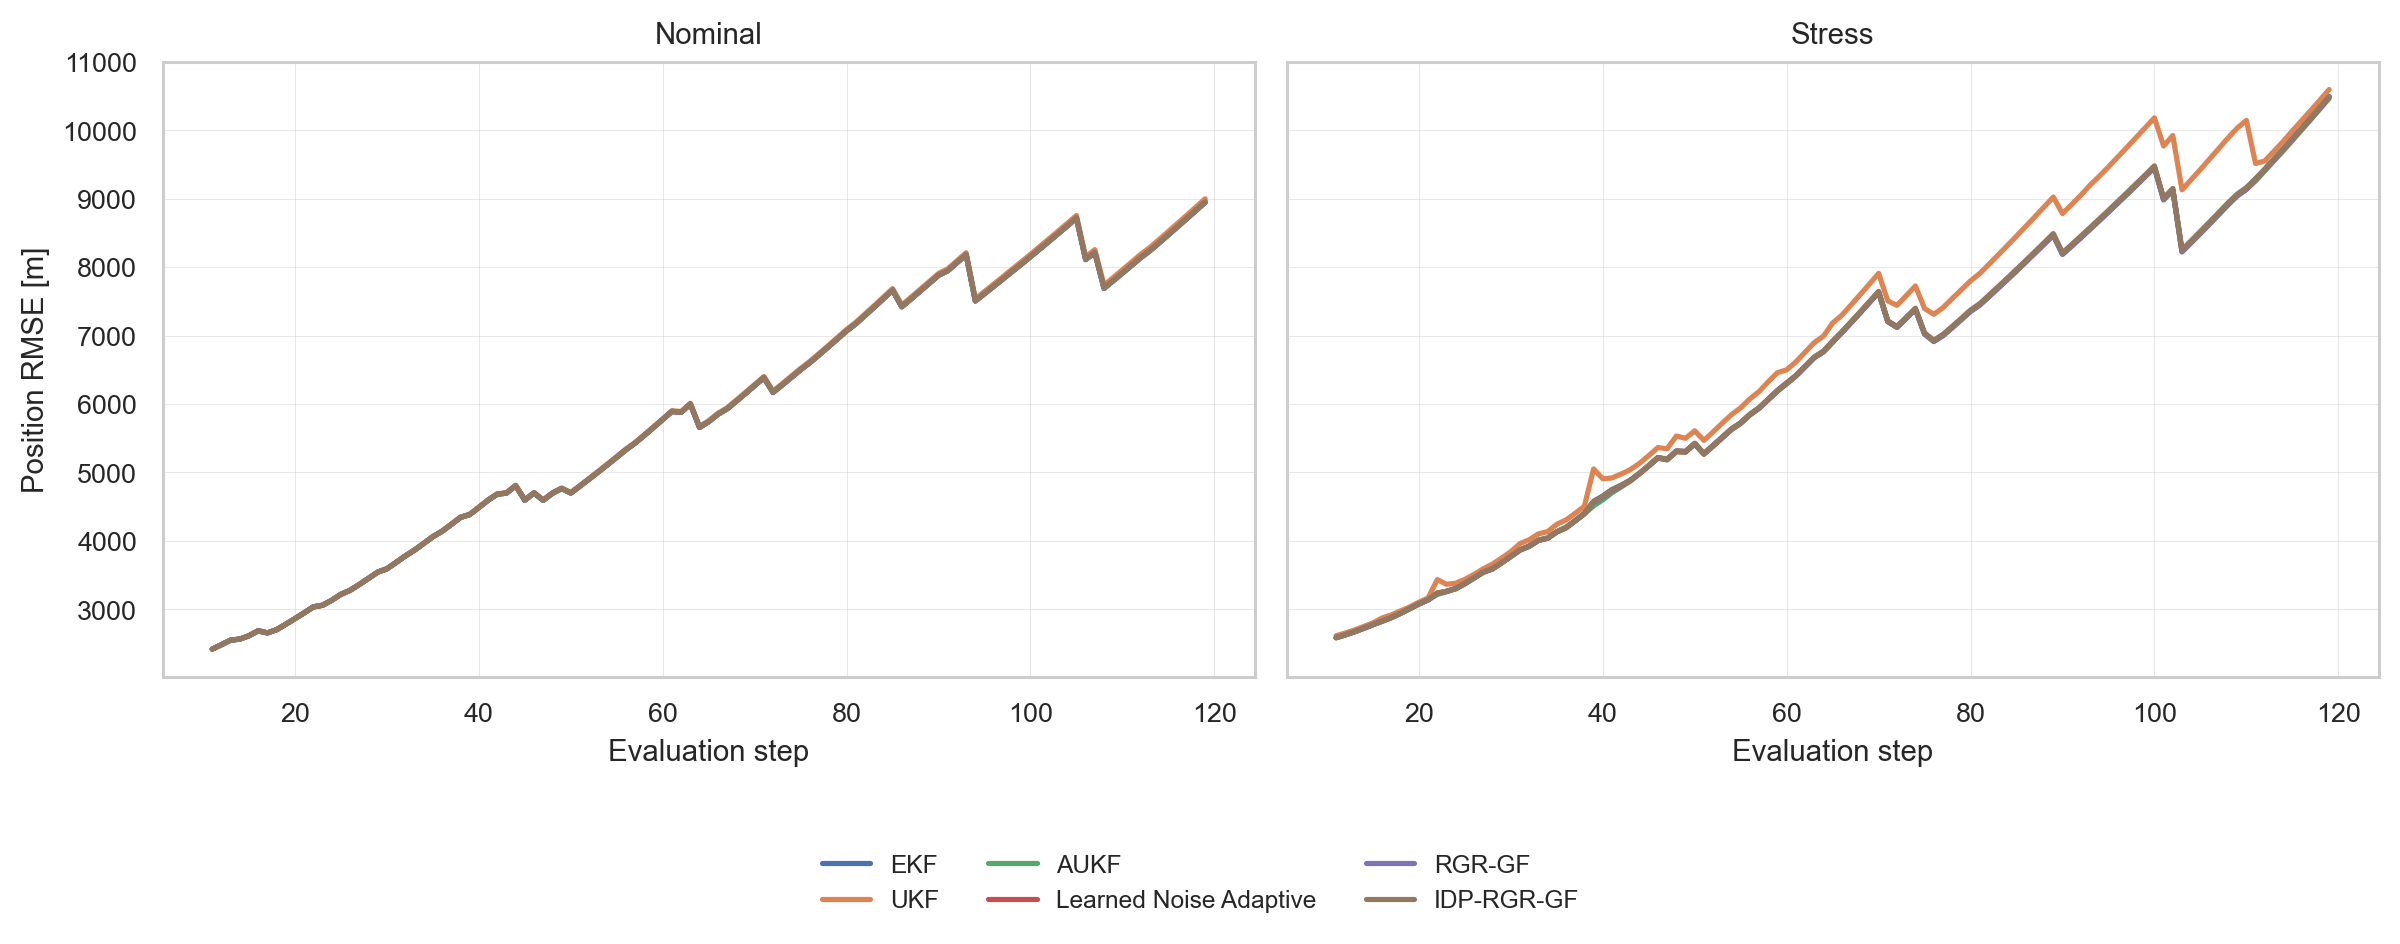
\includegraphics[width=0.48\textwidth]{figures/per_step_rmse.png}
  \caption{Per-step position RMSE over the nominal and stress evaluation windows. The curves are propagation-dominated; stress-split RMSE grows from about 2.59~km at the first scored step to about 10.47~km (AUKF), 10.48~km (RGR-GF), and 10.59~km (fixed-noise UKF), consistent with S-Table~\ref{tab:main_results}. Temporal diagnostic only.}
  \label{fig:per_step_rmse}
\end{figure}

\begin{figure}[htbp]
  \centering
  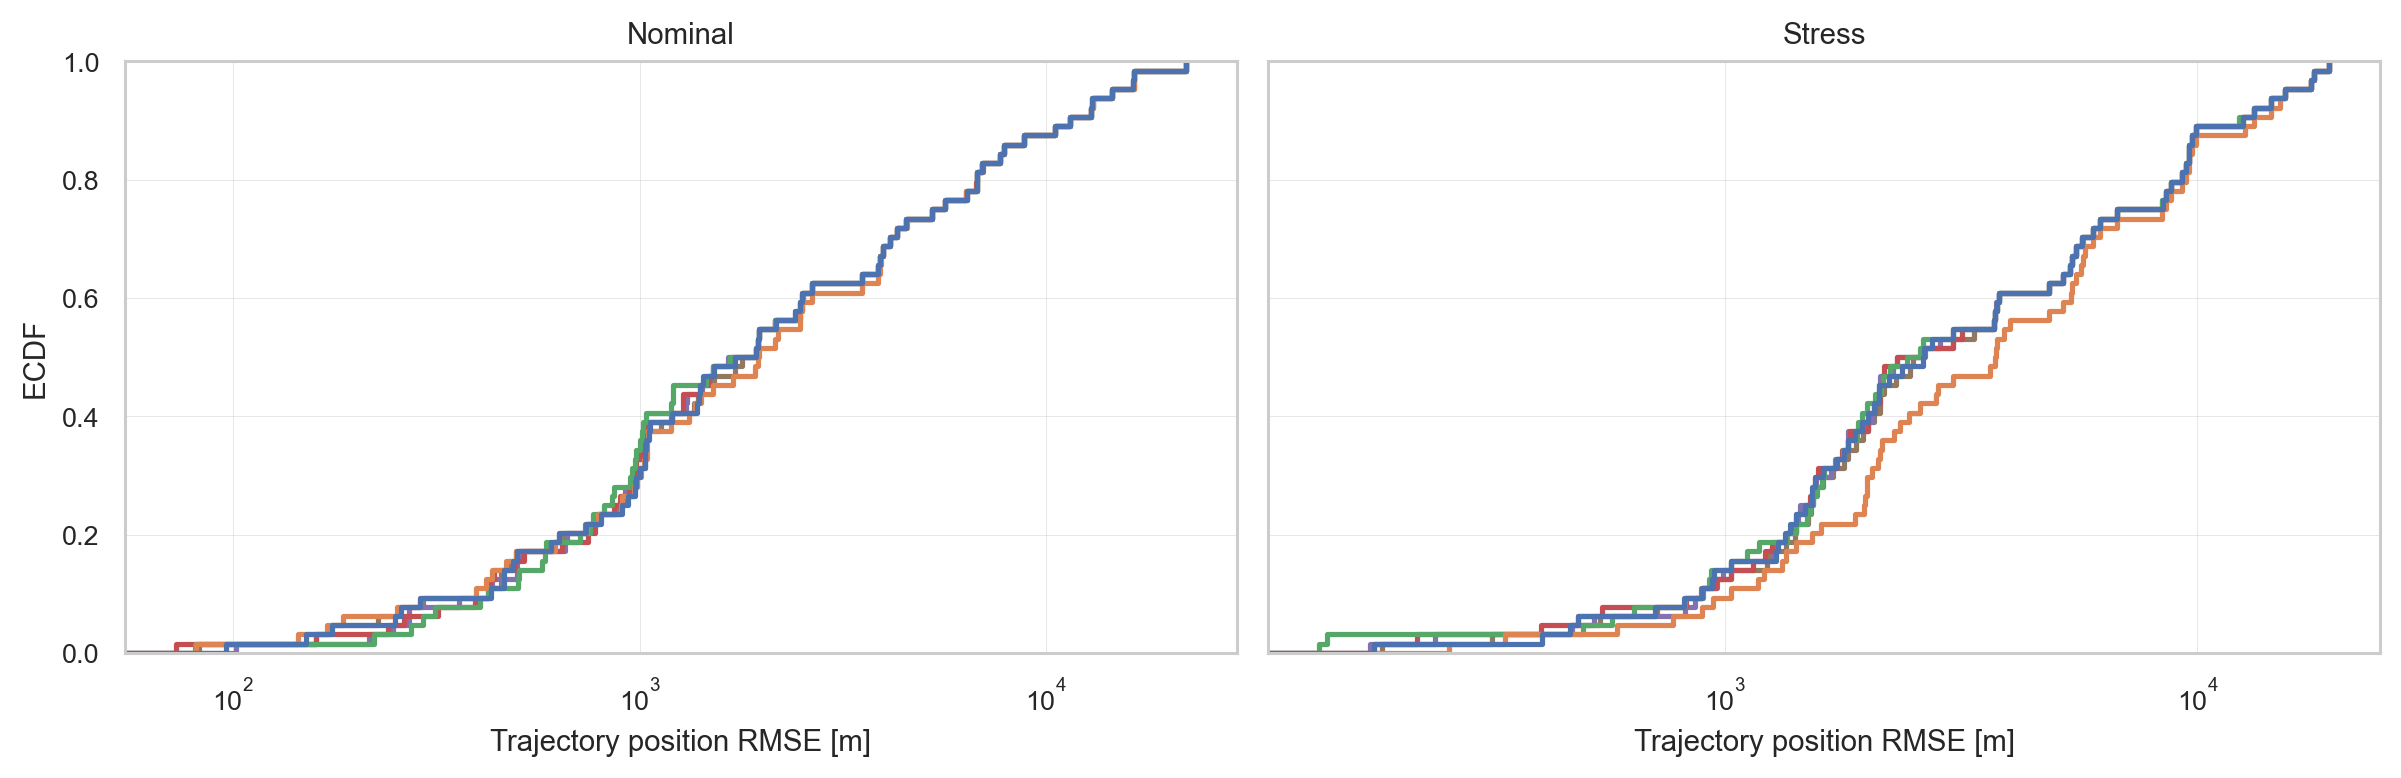
\includegraphics[width=0.48\textwidth]{figures/position_error_ecdf.png}
  \caption{Empirical cumulative distribution of trajectory-step position error (m). On the stress split the median trajectory RMSE is about 2.51~km (AUKF), 2.47~km (RGR-GF), and 3.74~km (fixed-noise UKF), while the 90th-percentile tail remains about 11.6--13.0~km for all three, so the learned model mainly reduces fixed-noise-UKF degradation without creating a new tail-safety regime.}
  \label{fig:position_error_ecdf}
\end{figure}

\begin{figure}[htbp]
  \centering
  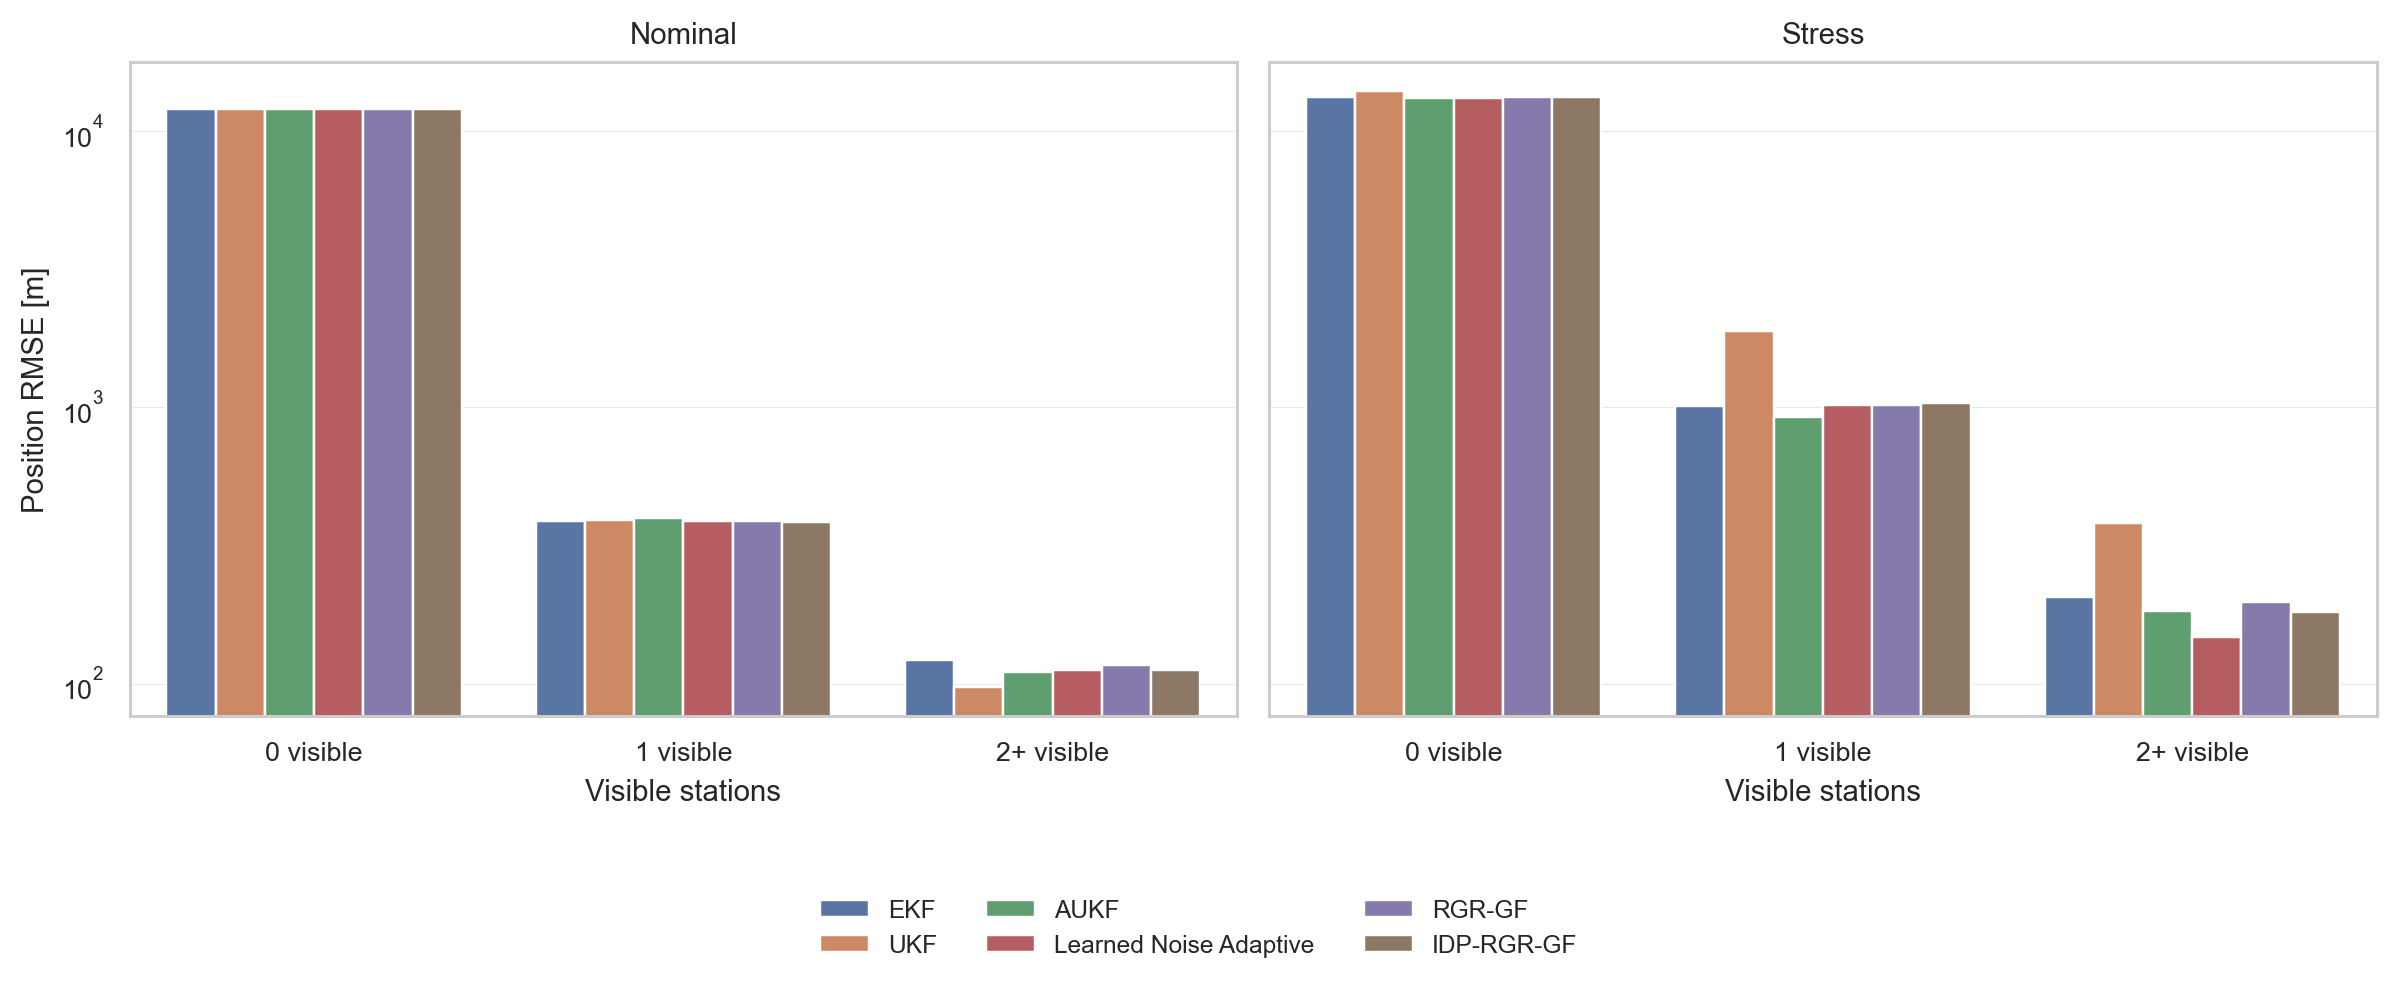
\includegraphics[width=0.48\textwidth]{figures/visibility_bucket_rmse.png}
  \caption{Position RMSE stratified by visibility bucket (0, 1, or $\geq2$ visible stations) for the nominal and stress settings. Diagnostic evidence for the evaluated runs only.}
  \label{fig:visibility_bucket_rmse}
\end{figure}

\begin{figure}[htbp]
  \centering
  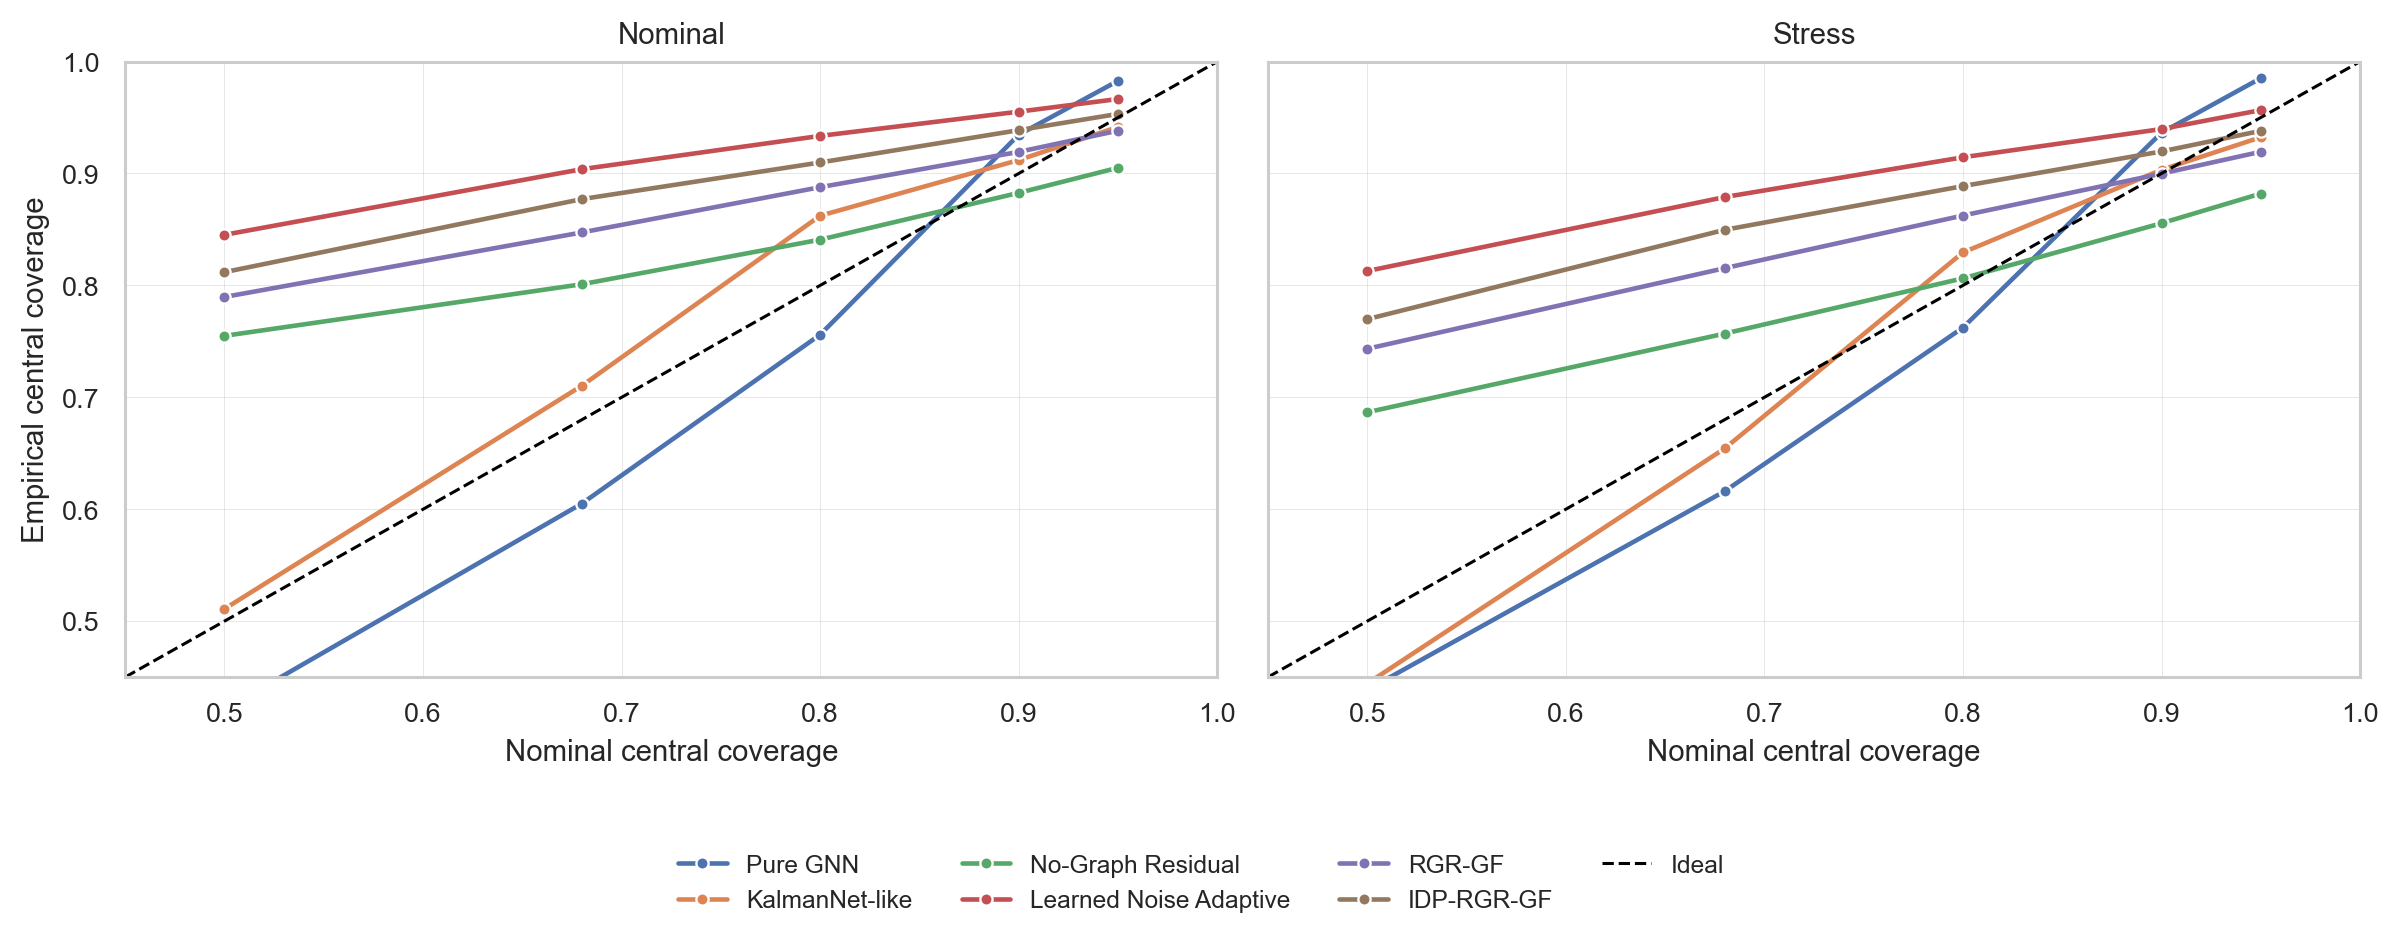
\includegraphics[width=0.48\textwidth]{figures/uncertainty_calibration.png}
  \caption{Uncertainty calibration diagnostic for the evaluated runs, comparing nominal and empirical central coverage for learned position uncertainty; interpreted as diagnostic evidence, not a deployment guarantee.}
  \label{fig:uncertainty_calibration}
\end{figure}

\bibliographystyle{plain}
\bibliography{references}

\end{document}

